%%%%%%%%%%%%% Partie obligatoire du préambule
\documentclass[a4paper,12pt,twoside]{book}
\usepackage{fontspec}
\usepackage{xunicode}
\usepackage[french]{babel}

%%%%%%%%%%%%%%%%%%%%%%%%%%%%%%%%% PACKAGES UTILISÉS

% Chargement du package biblatex
\usepackage{url}
\usepackage{csquotes} % les guillemets français
\usepackage[
    left = \flqq{},% 
    right = \frqq{},% 
    leftsub = \flq{},% 
    rightsub = \frq{} %
]{dirtytalk}

\usepackage{lettrine} %faire une lettrine (pas obligatoire)
\usepackage[style=enc,sorting=nyt,maxbibnames=10]{biblatex}%charger le style de l'EnC (téléchargeable ici https://ctan.org/pkg/biblatex-enc)
\addbibresource{Bibliographie/Senat.bib}
\addbibresource{Bibliographie/Automatisation.bib}

\DeclareSourcemap{%
 \maps[datatype=bibtex]{%
 	\map[overwrite]{%
 		\perdatasource{Bibliographie/Senat.bib}
 		\step[fieldset=keywords, fieldvalue={,senat}, append]
 	}
	\map[overwrite]{%
		\perdatasource{Bibliographie/Automatisation.bib}
		\step[fieldset=keywords, fieldvalue={,auto}, append]
	}	
  }
}
 
\nocite{*}
\defbibnote{intro}{Cette bibliographie présente toutes les ressources utilisées, de tout type, citées ou non, par simple ordre alphabétique.}

%%%%%%%%%%%%%%%%%%%%%%%%%%%%%%%%% AJOUT DE PACKAGE
\usepackage{graphicx} % Pour les insertions d'images
\usepackage{adjustbox} % Pour adapter la taille des images
\usepackage{lscape}
\usepackage{float}
\usepackage{tabularx} % Package pour un tableau ajustable
%\usepackage{tocbibind} % pour l'inclusion de la liste des figures etc à la table des matière
\usepackage{verbments} % For verbatim inside tabular
\usepackage[table]{xcolor} % Pour la coloration des tableaux et du texte
\usepackage{array} % Pour la gestion des tableaux. Le type de colonne m{}, permet de centrer verticalement le texte dans les cellules.
\usepackage{pdfpages} % Pour inclure des fichiers PDF (annexe 2)
\usepackage{tocbibind} % Pour inclure les annexes dans la table des matières
\usepackage{longtable}  % Gói này sẽ giúp xử lý các bảng dài.
\usepackage{makecell}   % Gói này giúp điều chỉnh kích thước ô và tự động xuống dòng.

\usepackage{titlesec}

% Tạo một cấp mới nhỏ hơn subsubsection (ví dụ như subsubsubsection)
\titleclass{\subsubsubsection}{straight}[\subsubsection]
\newcounter{subsubsubsection}[subsubsection]
\renewcommand\thesubsubsubsection{\thesubsubsection.\arabic{subsubsubsection}}
\titleformat{\subsubsubsection}
  {\normalfont\normalsize\bfseries}{\thesubsubsubsection}{1em}{}

\titlespacing*{\subsubsubsection}{0pt}{1.5ex plus 1ex minus .2ex}{1.5ex plus .2ex}

%%%%%%%%%%%%%%%%%%%%%%%%%%%%%%%%% CONFIGURATION DE MISE EN PAGE

%%%%%% Les compteurs (sections, subsections, etc)
%\renewcommand{\thesection}{\Roman{section}.}%On ne fait apparaître que le numéro de la section
%\renewcommand{\thesubsection}{\arabic{subsection}.}%subsection en chiffres arabes
%\renewcommand{\thesubsubsection}{\alph{subsubsection}.}%subsubsection en lettres minuscules
%Si l'on veut faire apparaître les subsubsection dans le table des matières (à commenter sinon)
\setcounter{tocdepth}{3}

%%%%%% Mise en page École des chartes
\usepackage[margin=2.5cm]{geometry}
\usepackage{setspace}
\onehalfspacing % interligne de 1.5
\setlength\parindent{1cm}

% Pour retirer le titre courant d'une page vide avant un chapitre
\newcommand{\clearemptydoublepage}{\newpage{\pagestyle{empty}\cleardoublepage}}

%%%%% Mise en forme des en-têtes et pieds de page
\usepackage{fancyhdr}
\usepackage{lastpage}
\pagestyle{fancy}

\renewcommand{\headrulewidth}{0pt}
\fancyhead[LO]{\rightmark}
\fancyhead[RO]{}
\fancyhead[RE]{\leftmark}
\fancyhead[LE]{}
\fancyfoot[C]{\thepage}

\renewcommand{\headrulewidth}{0pt}
\renewcommand{\chaptermark}[1]{\markboth{#1}{}}


\setlength\headheight{16pt} % la hauteur des headers
\renewcommand{\sectionmark}[1]{\markright{\small\textit{\thesection~\  #1}}} % Faire apparaître dans les headers les sections en petit et en italiques
\renewcommand{\chaptermark}[1]{\markboth{\small\chaptername~\thechapter~--\ \textit{#1}}{}} % idem pour les chapitres

% Package hyperref
\usepackage[xetex]{hyperref} % Inclure hyperref une seule fois
\hypersetup{
	pdfauthor = {Prénom Nom},
	pdftitle = {Titre du Document},
	pdfsubject = {Mémoire TNAH — Titre},
	pdfkeywords = {automatisation, python, pdfplumber, regex, tables du senat, journal officiel, séance publique}, % Séparer les mots-clés par des virgules
	colorlinks = false, % Pour que les liens n'aient pas de couleur
	breaklinks = true, % Permet aux liens d'être sur plusieurs lignes
	}
% Package bookmark, à mettre après hyperref
\usepackage[numbered]{bookmark} % Les signets seront numérotés
% Blocs de code
\usepackage{listings}

% Định nghĩa các màu sắc
\definecolor{purple}{rgb}{0.58, 0.0, 0.83}     % Màu tím cho từ khóa đặc biệt như from, import
\definecolor{blue}{rgb}{0.0, 0.0, 1.0}         % Màu xanh dương cho từ khóa như def, True, False, etc.
\definecolor{yellow}{rgb}{1.0, 0.84, 0.0}      % Màu vàng cho tên hàm khai báo, print, quit, range, len
\definecolor{red}{rgb}{1.0, 0.0, 0.0}          % Màu đỏ cho chuỗi ký tự, đường dẫn, URL
\definecolor{green}{rgb}{0.0, 0.5, 0.0}        % Màu xanh lá cho comment
\definecolor{black}{rgb}{0.0, 0.0, 0.0}        % Màu đen cho các phần còn lại
\definecolor{graybackground}{rgb}{0.95, 0.95, 0.95}  % Màu nền xám nhạt

% Thiết lập hiển thị code Python cho toàn bộ tài liệu
\lstset{
    language=Python,
    basicstyle=\ttfamily\small,          % Font monospace
    keywordstyle=\color{purple}\bfseries, % Từ khóa màu tím (from, import, if, while,...)
    keywordstyle=[2]\color{blue},        % Từ khóa màu xanh dương cho các từ như def, True, False, range, len, open...
    commentstyle=\color{green}\itshape,  % Comment màu xanh lá
    stringstyle=\color{red},             % Chuỗi ký tự màu đỏ
    identifierstyle=\color{black},       % Biến/hàm màu đen
    showstringspaces=false,              % Ẩn khoảng trắng trong chuỗi
    backgroundcolor=\color{graybackground}, % Nền màu xám nhạt
    frame=single,                        % Khung xung quanh mã
    breaklines=true,                     % Xuống dòng tự động khi mã quá dài
    numbers=none,                        % Không đánh số dòng
    tabsize=4,                           % Kích thước tab
    captionpos=b,                        % Đặt caption ở dưới cùng
    morekeywords={from, import, if, while, try, break, except, return, elif, with, for, as}, % Từ khóa màu tím
    morekeywords=[2]{def, not, True, False, (), f, range, len, open, in, r}, % Từ khóa màu xanh dương (def, True, False...)
    emph={print, quit, range, len},      % Từ khóa cần tô màu vàng (print, quit, range, len)
    emphstyle=\color{yellow}\bfseries,   % Màu vàng cho các từ khóa quan trọng
    emph={[2]extract_bold_lines_from_all_pages}, % Tên hàm khai báo màu vàng
    emphstyle={[2]\color{yellow}\bfseries},
    morestring=[b]", % Chuỗi ký tự màu đỏ
    morestring=[b]', 
}

\lstdefinelanguage{XML}
{
	basicstyle=\ttfamily, % Style de base pour le texte du code
	morestring=[b]", % Identification des chaînes de caractères entre guillemets doubles
	morestring=[s]{>}{<}, % Identification des chaînes entre '>' et '<' 
	identifierstyle=\color{blue}, % Couleur des noms de balises
	keywordstyle=\color{orange}, % Couleur des mots clés
	commentstyle=\color{green}, % COuleur des commentaires 
	moredelim=[s][\color{red}]{\ }{=}, % Définition des délimiteurs pour les attributs (espaces suivis d'un signe "=")
	stringstyle=\color{orange}, % COuleur des chaînes de caractères
	moredelim=[s][\color{black}]{>}{<}, % Définition des délimiteurs pour les balises (entre '>' et '<') en noir
	showspaces=false,  % Ne pas montrer les espaces
	frame=tb, % Cadre en haut et en bas
	breaklines=true, % Couper les lignes trop longues
	tabsize=2  % Taille des tabulations}
}

% Définition d'un environnement pour le code XML
\lstnewenvironment{xml}
{
	% Applique le style de code XML et défini la police et la taille du texte, permet aux chaînes de casser automatiquement en fin de ligne, 
	\lstset{language=XML, basicstyle=\ttfamily\small, breaklines=true}
}
{}

% Définition d'un style pour le code XML appelé dans le texte
\newcommand\xmlstyle{\lstset{
		language=XML,
		basicstyle=\ttfamily,
		keywordstyle=\color{orange},
		stringstyle=\color{orange},
		identifierstyle=\color{blue},
		commentstyle=\color{green},
		moredelim=[s][\color{red}]{\ }{=},
		moredelim=[s][\color{black}]{>}{<},
}}
% Glossaire
\usepackage[toc=true]{glossaries}
\makeglossaries

% Définitions du glossaire
\newglossaryentry{groupes_politiques}{
    name={Groupes politiques},
    description={Les groupes politiques au Sénat sont des regroupements de sénateurs par affinités politiques. Chaque sénateur appartient à un groupe, sauf s'il est non-inscrit. Ces groupes sont proportionnellement représentés selon leur importance numérique et jouent un rôle crucial dans les débats et les votes.}
}

\newglossaryentry{bureau_senat}{
    name={Bureau du Sénat},
    description={Le Bureau du Sénat est un organe collégial composé de 26 membres : le Président du Sénat, 8 Vice-présidents, 3 Questeurs et 14 Secrétaires. Il est chargé de prendre les décisions relatives à l'organisation et au fonctionnement interne du Sénat. La composition reflète la représentation proportionnelle des groupes politiques.}
}

\newglossaryentry{commissions_permanentes}{
    name={Commissions permanentes},
    description={Les commissions permanentes sont des organes législatifs au sein du Sénat composés de sénateurs issus des différents groupes politiques. Elles sont chargées d'examiner les projets de loi et de proposer des amendements avant leur discussion en séance publique.}
}

\newglossaryentry{commissions_temporaires}{
    name={Commissions temporaires},
    description={Les commissions temporaires sont créées pour traiter des sujets ponctuels ou urgents. Leur composition varie en fonction des thématiques à aborder et de la disponibilité des sénateurs compétents.}
}

\newglossaryentry{delegations_structures}{
    name={Délégations et autres structures parlementaires},
    description={Les délégations parlementaires sont des groupes chargés de suivre des thématiques spécifiques, telles que les droits des femmes ou le renseignement. Elles complètent le travail des commissions permanentes en approfondissant certains dossiers.}
}

\newglossaryentry{changements_organes}{
    name={Changements au sein des organes},
    description={Les changements dans les commissions, délégations et autres organes surviennent après les élections sénatoriales ou des ajustements internes. Ces modifications visent à refléter les nouvelles configurations politiques et les besoins institutionnels.}
}

\newglossaryentry{cour_justice_republique}{
    name={Cour de justice de la République},
    description={La Cour de justice de la République est une juridiction spéciale qui juge les ministres pour les infractions commises dans l'exercice de leurs fonctions. Elle est composée de parlementaires et de magistrats de la Cour de cassation.}
}

\newglossaryentry{organismes_extra_parlementaires}{
    name={Organismes extra-parlementaires},
    description={Les organismes extra-parlementaires incluent des instances consultatives dans lesquelles des parlementaires siègent pour orienter des politiques publiques. Ces organismes jouent un rôle clé dans le conseil aux agences publiques et aux commissions.}
}

\newglossaryentry{petitions}{
    name={Pétitions},
    description={Les pétitions permettent aux citoyens de soumettre directement des questions au Parlement. Elles sont examinées par des commissions qui décident des suites à donner, comme des débats ou des propositions de loi.}
}

\newglossaryentry{rapports}{
    name={Rapports remis au Parlement},
    description={Les rapports sont des documents rédigés par les commissions ou délégations parlementaires. Ils présentent des analyses ou des recommandations sur des sujets législatifs et peuvent aboutir à des propositions de loi.}
}


 \newglossaryentry{actionchains}{%
    name={ActionChains},%
    description={ActionChains est une classe dans la bibliothèque Selenium pour Python qui permet de créer et d'exécuter des séquences complexes d'interactions utilisateur, telles que cliquer, glisser-déposer, et double-cliquer, sur les éléments d'une interface graphique d'application web}}

\newglossaryentry{bert}{%
    name={BERT},%
    description={BERT (Bidirectional Encoder Representations from Transformers) est un modèle d'apprentissage profond basé sur les transformers, développé par Google, qui permet d'obtenir des représentations de texte contextuelles. BERT est particulièrement puissant pour les tâches de NLP telles que la classification de texte, la réponse à des questions, et l'analyse syntaxique}}

\newglossaryentry{xpath}{%
    name={XPath},%
    description={XML Path Language. Langage utilisé pour naviguer et sélectionner des éléments au sein d'une structure de document XML ou HTML. Il permet de désigner de manière précise des parties spécifiques d'un document en fonction de sa structure hiérarchique, comme des balises, des attributs ou des valeurs.}}


\newglossaryentry{selenium}{%
    name={Selenium},%
    description={Bibliothèque open-source utilisée principalement pour l'automatisation de tests de navigateurs web. Elle permet de simuler des interactions avec un navigateur, comme un utilisateur humain le ferait, ce qui la rend particulièrement utile pour tester des applications web de manière automatisée.}}

\newglossaryentry{csv}{%
    name={CSV},%
    description={Le CSV (Comma-Separated Values) est un format de fichier utilisé pour stocker des données tabulaires sous forme de texte brut. Chaque ligne du fichier représente une ligne de la table, et les valeurs de chaque colonne sont séparées par des virgules (ou par d'autres séparateurs, comme les points-virgules)}}

\newglossaryentry{dataframe}{%
    name={DataFrame},%
    description={Un DataFrame est une structure de données bidimensionnelle de type tableau, souvent utilisée dans les bibliothèques de manipulation de données comme Pandas en Python. Il permet de stocker et de manipuler des données en colonnes, où chaque colonne peut être de types différents (numériques, textuels, etc.)}}

\newglossaryentry{gliner}{%
    name={GLiNER},%
    description={Gliner est une méthode ou un outil utilisé pour l'automatisation ou l'optimisation de certains processus, mais les détails spécifiques peuvent dépendre du contexte d'application. Il pourrait être nécessaire de définir avec plus de précision en fonction du domaine où le terme est utilisé}}

\newglossaryentry{gliner-ner}{%
    name={Modèle NER Gliner},%
    description={Le modèle NER (Named Entity Recognition) Gliner est un modèle spécifique de reconnaissance d'entités nommées utilisé pour identifier et classer automatiquement des entités comme des personnes, des organisations, des dates ou des lieux dans un texte. Ce modèle peut être basé sur des approches d'apprentissage profond et est utilisé dans le traitement automatique du langage naturel (NLP) pour extraire des informations structurées à partir de données textuelles non structurées}}

\newglossaryentry{google-colab}{%
    name={Google Colab},%
    description={Google Colaboratory, communément appelé Google Colab, est un environnement de développement intégré basé sur le cloud qui permet d'exécuter du code Python directement dans le navigateur. Il est particulièrement utile pour les tâches nécessitant des ressources de calcul importantes, telles que l'entraînement de modèles d'apprentissage automatique. Google Colab permet d'accéder gratuitement à des GPU et TPU, facilitant ainsi l'expérimentation avec des projets de machine learning et de deep learning}}

\newglossaryentry{mypdf}{%
    name={mypdf},%
    description={\texttt{mypdf} est une bibliothèque Python utilisée pour la création, la lecture et la modification de fichiers PDF. Elle permet de générer des documents PDF à partir de zéro ou d'ajouter du contenu à des fichiers existants, comme du texte, des images, ou des annotations. \texttt{mypdf} prend en charge la manipulation des polices, des styles de texte, et des éléments graphiques, rendant ainsi possible l'automatisation de tâches telles que la génération de rapports ou de factures. Elle est également utilisée pour extraire des informations spécifiques à partir de fichiers PDF, comme des métadonnées ou du texte, ce qui en fait un outil polyvalent pour la gestion des documents électroniques}}

\newglossaryentry{ner}{%
    name={NER},%
    description={La reconnaissance d'entités nommées (NER, Named Entity Recognition) est une tâche de traitement du langage naturel (NLP) qui consiste à identifier et à classer les entités nommées dans un texte, telles que les noms de personnes, d'organisations, de lieux, de dates, de valeurs numériques, etc. Les modèles NER sont souvent utilisés pour l'extraction d'informations à partir de grandes quantités de données textuelles}}

\newglossaryentry{elementtree}{%
    name={ElementTree},%
    description={API intégrée dans Python pour la manipulation des fichiers XML. Elle fait partie du module xml.etree.ElementTree et permet de lire, écrire, parcourir et modifier des documents XML de manière simple et efficace.}}



\newglossaryentry{nlp}{%
    name={NLP},%
    description={Le traitement du langage naturel (NLP, Natural Language Processing) est un sous-domaine de l'intelligence artificielle qui s'intéresse à l'interaction entre les ordinateurs et les langues humaines. Il inclut des techniques pour l'analyse, la compréhension et la génération du langage humain naturel, utilisé notamment pour des tâches comme la traduction automatique, l'analyse de sentiments, et la reconnaissance d'entités nommées}}

\newglossaryentry{ocr}{%
    name={OCR},%
    description={La reconnaissance optique de caractères (OCR, Optical Character Recognition) est une technologie permettant de convertir des images de texte en texte codé. Elle est utilisée pour la numérisation de documents imprimés ou manuscrits, facilitant ainsi la recherche, l'édition et l'archivage de textes}}

\newglossaryentry{pandas}{%
    name={pandas},%
    description={Pandas est une bibliothèque open-source en Python largement utilisée pour la manipulation et l'analyse de données. Elle est particulièrement adaptée aux structures de données tabulaires, comme les feuilles de calcul ou les bases de données.}}

\newglossaryentry{pdf}{%
    name={PDF},%
    description={Le Portable Document Format (PDF) est un format de fichier développé par Adobe pour représenter des documents de manière indépendante du logiciel, du matériel et du système d'exploitation utilisé. Il est largement utilisé pour partager des documents électroniques tout en conservant la mise en forme, les polices, les images et autres éléments visuels}}

\newglossaryentry{pdfplumber}{%
    name={pdfplumber},%
    description={\texttt{pdfplumber} est une bibliothèque Python spécialisée dans l'extraction avancée de données à partir de fichiers PDF. Contrairement à d'autres bibliothèques qui se concentrent uniquement sur l'extraction de texte brut, \texttt{pdfplumber} permet également de capturer des éléments structurés tels que des tableaux, des images, des graphiques et même des figures complexes. Cette bibliothèque est particulièrement utile pour les utilisateurs qui ont besoin de traiter des documents PDF contenant des données tabulaires ou des diagrammes, comme des relevés bancaires, des factures ou des rapports techniques. Elle permet aussi de manipuler les fichiers PDF en identifiant et extrayant des sections spécifiques, tout en gérant les différences de mise en page et de structure entre les fichiers}}

\newglossaryentry{python}{%
    name={Python},%
    description={Le langage Python est un langage de programmation open source multi-plateformes et orienté objet. Grâce à des bibliothèques spécialisées, Python s'utilise à la fois pour le développement web, l'analyse de données, l'intelligence artificielle et la gestion d'infrastructures. Actuellement le plus utilisé au monde, ce langage est dit de \enquote{haut niveau} car il permet d'écrire des programmes en utilisant des mots usuels des langues naturelles et des symboles mathématiques familiers}}

\newglossaryentry{regex}{%
    name={Regex},%
    description={Les expressions régulières (Regex, Regular Expressions) sont des séquences de caractères qui définissent un modèle de recherche. Elles sont utilisées pour correspondre et manipuler des chaînes de caractères selon des motifs définis, permettant des tâches comme la validation de formats de données, la recherche et le remplacement de texte, ou l'extraction de sous-chaînes spécifiques dans des documents textuels}}

\newglossaryentry{spacy}{%
    name={spaCy},%
    description={spaCy est une bibliothèque de traitement du langage naturel en Python, optimisée pour la rapidité et l'efficacité. Elle fournit des outils de pointe pour les tâches de NLP comme la reconnaissance d'entités nommées, la lemmatisation, l'analyse de dépendances, et le tokenization. spaCy est largement utilisée dans des applications industrielles et de recherche en raison de sa simplicité d'utilisation et de ses performances élevées}}

\newglossaryentry{XML}{%
    name={XML},%
    description={Extensible Markup Language. Langage de balisage conçu pour créer des documents structurés et hiérarchisés à l’aide de balises définies par l'utilisateur, contrairement aux langages de balisage avec des balises prédéfinies. XML est principalement utilisé pour la gestion et l’échange d’informations, permettant de partager et de stocker des données de manière lisible pour les humains et les machines. Son objectif principal est de faciliter l'interopérabilité entre différents systèmes, notamment via Internet}}

\newglossaryentry{SQL}{%
    name={SQL},%
    description={Structure Query Language. Langage de requête structuré utilisé pour interagir avec des bases de données relationnelles.}}

\newglossaryentry{Prepub}{%
    name={Prepub},%
    description={Logiciel d'archivage interne du Sénat français pour saisie, analyse et publication du Journal Officiel.}}

\newglossaryentry{JO}{%
    name={Journal Officiel},%
    description={Conformément à l'article 33 de la Constitution, les séances du Sénat sont publiques et le compte rendu intégral des débats est publié au Journal Officiel.}}

\newglossaryentry{bornage}{%
    name={bornage},%
    description={Marquage des contenus du Journal Officiel en prévision d'une analyse des débats}}

\newglossaryentry{HTML}{%
    name={HTML},%
    description={HyperText Markup Language. Langage de balisage standard utilisé pour créer des pages web. Il permet de structurer le contenu d'une page en définissant des éléments tels que des titres, des paragraphes, des liens, des images et d'autres médias.}}

\newglossaryentry{PDF}{%
    name={PDF},%
    description={Portable Document Format. Format de fichier créé par Adobe Systems en 1993, destiné à représenter des documents de manière indépendante du logiciel, du matériel et des systèmes d'exploitation. Un fichier PDF peut contenir du texte, des images, des graphiques et d'autres éléments, tout en préservant la mise en forme d'origine du document.}}

\newglossaryentry{DILA}{%
    name={DILA},%
    description={Direction de l'Information Légale et Administrative. Direction d'administration centrale des services du Premier ministre, placée sous l'autorité du secrétariat général du Gouvernement.}}
\newglossaryentry{BERT}{
    name=BERT,
    description={Modèle de langage basé sur les transformateurs, développé par Google, utilisé pour le traitement du langage naturel (Traitement Automatique du Langage Naturel - TALN) et ayant une bonne capacité à comprendre le contexte.}
}

\newglossaryentry{spaCy}{
    name=spaCy,
    description={Bibliothèque open source pour Python, conçue pour le traitement du langage naturel (TALN), offrant des outils pour analyser le texte, identifier des entités, et bien d'autres fonctionnalités.}
}

\newglossaryentry{OCR}{
    name=OCR,
    description={Optical Character Recognition. La Reconnaissance Optique de Caractères est une technologie qui permet de convertir des images de texte imprimé, écrit à la main ou tapé, en texte numérique exploitable par des ordinateurs.}
}

\newglossaryentry{open-source}{
    name=open-source,
    description={Modèle de développement logiciel dans lequel le code source d'un programme est rendu accessible à tous. Cela signifie que tout utilisateur peut voir, modifier, améliorer ou redistribuer le logiciel selon ses besoins, tant que cela respecte les conditions de la licence sous laquelle il est publié.}
}

\newglossaryentry{ChatGPT}{
    name=ChatGPT,
    description={Generative Pretrained Transformer. ChatGPT est un modèle de traitement du langage naturel développé par OpenAI. Il utilise l'intelligence artificielle pour comprendre et générer du texte en langage naturel, permettant aux utilisateurs d'interagir avec lui via des conversations textuelles.}
}
\newglossaryentry{Gliner}{
    name=Gliner,
    description={Global Linearization Network with Embedding Representations. Modèle de reconnaissance d'entités nommées (NER) avancé dans le domaine du traitement du langage naturel (NLP). Ce modèle est conçu pour identifier et catégoriser des entités dans un texte, comme des personnes, des organisations, des lieux, des dates, et bien d'autres.}
}

\newglossaryentry{Tesseract}{
    name=Tesseract,
    description={Bibliothèque open-source dédiée à la Reconnaissance Optique de Caractères (OCR). Initialement développée par Hewlett-Packard dans les années 1980, Tesseract est maintenant maintenue par Google. Elle permet de convertir des images contenant du texte en fichiers texte numériques exploitables, tout comme d'autres outils OCR..}
}

\newglossaryentry{CSV}{
    name=CSV,
    description={Format de fichier texte simple où chaque ligne correspond à un enregistrement, et les champs dans l'enregistrement sont séparés par des virgules (Valeurs Séparées par des Virgules). Utilisé couramment pour stocker des données tabulaires.}
}

\newglossaryentry{cloud}{
    name=cloud,
    description={Informatique en nuage en français, désigne l'utilisation de serveurs distants via Internet pour stocker, gérer et traiter des données, au lieu de les gérer sur des serveurs locaux ou des ordinateurs personnels.}
}

\newglossaryentry{bibliothèque}{
    name=bibliothèque,
    description={Library en anglais. Ensemble de fonctions, classes ou modules préécrits qui peuvent être réutilisés par les développeurs dans leurs propres programmes. Elle permet de simplifier le développement en fournissant des outils prêts à l'emploi pour accomplir des tâches spécifiques, comme la gestion des entrées/sorties, les calculs mathématiques, la manipulation de fichiers, ou encore l'interaction avec des bases de données.}
}


% Création de l'environnement pour citer
\newenvironment{kwote}
{
	\begin{quote}
		\begin{singlespace}
			\small
		}
		{
			\normalsize
		\end{singlespace}
	\end{quote}
}


%%%%%%%%%%%%%%%%%%%%%% DOCUMENT
\begin{document}
	\onehalfspacing 
	
	\frontmatter
	
	\author{Le Thuy Tien Nguyen - M2 TNAH}
\title{Titre du mémoire}

%\documentclass[a4paper]{article} 

%\usepackage[utf8]{inputenc} 
%\usepackage[T1]{fontenc}
%\usepackage{graphicx} 
%\usepackage[top=3cm, bottom=3cm, left=3cm, right=3cm]{geometry} 
%\usepackage{relsize} % Để sử dụng \larger, \Large, \Huge
%\usepackage{csquotes} % Để sử dụng \enquote

%\begin{document}

\begin{titlepage} 

\centering 

{\LARGE ÉCOLE NATIONALE DES CHARTES\\
UNIVERSITÉ PARIS, SCIENCES \& LETTRES \par} 

\vspace{1cm} % Điều chỉnh khoảng trắng nếu cần
\rule{2cm}{0.02cm}

\vspace{3cm} 

{\Large \textbf{Le Thuy Tien NGUYEN} \par}

\normalsize \textit{licenciée ès histoire} \par

\vspace{2cm} 

{\Huge \textbf{Donner accès aux débats parlementaires au Sénat. Les enjeux de l’automatisation de la création des tables des matières pour les sessions parlementaires } \par}

\vspace{1cm}

{\LARGE \textbf{L’exemple des Journaux Officiels 2022.} \par}

\vfill

{\large Mémoire pour le diplôme de master \par}
{\large « Technologies numériques appliquées à l'histoire » \par} 

\vspace{0.5cm}

{2024 \par} 

\end{titlepage}
	\thispagestyle{empty}
	\clearemptydoublepage

	\chapter*{Résumé}
\medskip
Ce mémoire explore l'automatisation de la création des tables des matières pour les débats parlementaires aux archives du Sénat, en se basant sur les Journaux Officiels de 2022. Le projet, réalisé dans le cadre d'un stage de six mois, vise à simplifier la gestion des métadonnées grâce à des outils d'intelligence artificielle et de traitement du langage naturel. Ce mémoire souligne l'importance de rendre les données accessibles tout en réduisant le temps de traitement manuel.
Grâce à des bibliothèques Python comme pdfplumber et des outils de traitement de texte comme Regex, il a été possible d'extraire automatiquement des informations pertinentes de documents PDF, comme le nom des intervenants et les textes de lois. Bien que certaines limites techniques, comme la reconnaissance d'entités spécifiques et la qualité des données sources, aient persistées, les résultats démontrent une nette amélioration en termes de précision et de rapidité par rapport à une saisie manuelle.
Le mémoire conclut que cette méthode d’automatisation ouvre des perspectives intéressantes pour le futur, notamment pour d'autres corpus de données parlementaires. Cependant, des avancées techniques supplémentaires, comme l'intégration de modèles d'apprentissage plus sophistiqués, et l'utilisation de matériel plus optimisés pour le traitement de l'IA, seraient nécessaires pour surmonter les défis actuels. .\\
	
\textbf{Mots-clés:} automatisation; intelligence artificielle; traitement du langage naturel; Sénat; Journaux Officiels; tables des matières; Python; extraction de texte, pdfplumber; regex.
	
\textbf{Informations bibliographiques:} Le Thuy Tien NGUYEN, \textit{Donner accès aux débats parlementaires au Sénat. Les enjeux de l’automatisation de la création des tables des matières pour les sessions parlementaires. L’exemple des Journaux Officiels 2022.}, mémoire de master \enquote{Technologies numériques appliquées à l'histoire}, directrice Marie PUREN, École nationale des chartes, 2024.
	\thispagestyle{empty}
	\clearemptydoublepage


	\chapter*{Remerciements}

Un mémoire est un parcours intellectuel exigeant et parfois solitaire, mais heureusement pour moi, j'ai eu la chance d'avoir de nombreux professeurs, directeurs, proches et amis qui ont tous contribué à enrichir ce projet et à stimuler ma curiosité. 
Je souhaite tout d'abord remercier mes professeurs à l'ENC-PSL, qui m'ont nourri avec des théories et des méthodes pratiques me permettant d'accéder aux moyens techniques dont j'avais besoin, tout en éclairant ma pensée par des connaissances élargies. J'ai acquis des outils pour m'entraîner et pratiquer au cours de ce stage, outils qui constituent maintenant les clés de ma future carrière.

Je remercie également Jean-Marc TICHI et Laurent BAOUR, qui m'ont accueilli en stage aux Archives du Sénat, notamment pour ce projet d'automatisation des Tables du Sénat. Je tenais à communiquer une mention toute spéciale à Laurent BAOUR, mon maître de stage, qui a toujours été présent pour m'aider à développer mes compétences durant ce stage. Il m'a prodigué de nombreux conseils et explications sur les bases du Sénat, mais également sur la science politique et a été mon lien pour échanger avec toute l'équipe des archivistes. Je remercie aussi les équipes opérationnelles, qui réalisent l'analyse et le bornage des Journaux Officiels, de m'avoir ouvert leurs portes et généreusement partagé leur vision de ce travail et leurs besoins professionnels. Échanger avec eux m'a ainsi permis de mieux comprendre leurs attentes et donner un sens plus humain à ma mission d'automatisation.

Bien entendu, je souhaite remercier ma directrice de mémoire, Marie PUREN, qui m'a guidé dans le développement de mon corpus ainsi que de mon livrable technique. J'ai apprécié tout particulièrement l'équilibre qu'elle a su établir entre la résolutions des enjeux du stage et ma liberté d'explorer les méthodes techniques qui me semblaient les plus appropriées. Sans ses commentaires avisés et ses références de qualité, mon mémoire aurait sans doute pris beaucoup plus de temps à atteindre un tel niveau de rigueur scientifique. Au-delà de son accompagnement, je lui suis très reconnaissante pour sa patience et sa tolérance.

Je tiens également à témoigner ma gratitude à Emmanuelle BERMES, responsable de master, qui m'a fait confiance et sans qui je n'aurais pas pu rejoindre ce parcours académique. Elle m'a soutenue et conseillée tout au long de cette année, toujours à l'écoute et prête à me rassurer, elle a su, à travers nos échanges, raviver ma motivation, m'aidant à entrevoir de nouvelles perspectives à mes études ainsi que sur mes choix. Ce travail n'aurait pas pu être réalisé sans son soutien moral et sa confiance. Je lui suis également très reconnaissante d'avoir tenu compte de mes besoins d'apprentissage aussi bien académiques que émotionnels. Sa capacité à comprendre ma situation, en tant qu'expatriée, m'a permis de garder ma motivation dans les moments où j'en avais le plus besoin.

Je suis également très reconnaissante envers ma famille, qui m'a soutenu tant sur le plan matériel que moral, malgré la distance.
Je remercie également mes amis, Giang et Vy, qui m'ont soutenu et encouragé avec intérêt. Je remercie aussi Hưng et Guillaume, qui ont gentiment accepté de m'aider à débugguer mon code à plusieurs reprises. Je suis reconnaissante envers Thomas, qui m'a écoutée avec patience, qui a toléré mes moments de morosité, sans jamais cesser de m'encourager à communiquer ce que je ressentais, merci de toujours être là.
	\clearemptydoublepage

%%%%%%%%%%%% \bibliographie ici (normes de l'EnC)
        \chapter{Bibliographie}
        \section*{Documentations du Sénat}
        \printbibliography[keyword=senat,heading=none]
        \section*{Automatisation}
        \printbibliography[keyword=auto,heading=none]
        \clearemptydoublepage


	%%%%%%%%%%%%%%%%%Le corps du mémoire
        \mainmatter

	\chapter*{Introduction}
\markboth{Introduction}{}
\addcontentsline{toc}{chapter}{Introduction}
\label{sec:introduction}

Rendre compte de l’activité parlementaire est une mission qui remonte à l’Antiquité, par exemple en Mésopotamie, où l’histoire et la société de ces cités nous est parvenues grâce « au déchiffrement [...] de petites tablettes d’argile couvertes d’écritures cunéiformes », dont certaines permettent de mieux comprendre « l’existence d’assemblées populaires […] représentatives de la population de la cité ».\footcite{HistoireSeance}. La retranscription des débats et leur publication était déjà à l’époque un enjeu politique majeur ; nous devons d’ailleurs à Jules César la publication du premier équivalent à un Journal Officiel en 59 avant J.-C. « Pour se rendre populaire, mais aussi pour contrôler l’information, [il] démocratisa ce système qui avait jusque-là été réservé à une élite ».\footcite{HistoireSeance}.
Plus récemment encore, car les temps changent, et que les comptes rendus de séance ne jouent plus le même rôle social qu’auparavant, nous pouvons constater trois phénomènes :
1/ Le déclin populaire de la séance publique qui concerne toutes les démocraties et affecte,
par contrecoup, les enjeux des débats.
2/ L’émergence de nouveaux moyens de communication, qui ont permis au contraire de donner une nouvelle portée à l’exigence de publicité.
3/ La vitalité qui continue d’animer des comptes rendus écrits désormais profondément rénovés. \footcite{HistoireSeance}

De nos jours, la séance publique est un moment clé de l’activité parlementaire, elle se déroule dans l’hémicycle du Sénat, où les décisions des Sénateurs sur les sujets examinés sont publiquement annoncées. Ces séances sont publiques, et les comptes rendus des débats sont publiés intégralement dans le Journal officiel, conformément à l’article 33 de la Constitution française. \footcite{article33}
Quant au Journal officiel, il n’est plus guère lu du grand public, [...] et même si les parlementaires y font encore fréquemment référence pour attester de leur activité, il s’adresse désormais à certains groupes spécialisés – juristes, administrateurs, consultants, magistrats, hommes politiques, groupes de pression et lobbies – qui en font le meilleur usage. \footcite{HistoireSeance}
À partir de l’analyse des débats en séance publique, et en commission pour la table nominative depuis avril 2009, les tables sont mises à jour chaque année. Elles classent les Sénateurs par nom et récapitulent, pour chacun d’eux, l’ensemble de leurs nominations et interventions en séance publique, telles que les thèmes abordés, les amendements déposés et les explications de vote. \footcite{HistoireSeance}
Les tables des matières jouent un rôle crucial dans la structuration et la consultation des documents officiels des sessions parlementaires. Elles permettent un accès rapide et organisé aux informations clés, facilitant ainsi le travail des législateurs, des chercheurs et des citoyens intéressés par les débats et décisions prises. La précision et la clarté de ces tables sont essentielles pour garantir une navigation fluide au sein de documents souvent volumineux et complexes.

Ces table sont traditionnellement remplies à la main par les archivistes du Sénat qui répertorient une par une les interventions de chaque sénateur, le sujet de leur prise de parole, l'article discuté et retranscrivent le contenu de leur prise de parole.
C’est justement la nécessité de mobiliser autant de ressources humaines dans ce travail d'archivage de la parole publique qui a motivé le choix de sujet de ce mémoire, afin d’explorer des solutions d’automatisation de ce processus indispensable au bon fonctionnement de notre démocratie.

L’automatisation des tables, visée par l’équipe des archivistes, a pour objectif non seulement d’alléger le travail manuel associé à leur création, mais aussi d’améliorer la cohérence et l’exactitude des informations présentées. L’enjeu principal est de pouvoir générer ces tables plus rapidement, tout en maintenant une haute qualité d’organisation et de présentation des données. Cela permettrait également une mise à jour plus fréquente et plus dynamique, offrant ainsi un accès quasi instantané aux informations les plus récentes.
Nous nous interrogeons donc sur le point suivants :  En quoi les méthodes actuelles de création de tables des matières pour les sessions peuvent-elles être améliorées grâce à l’automatisation ? L’automatisation pourrait-elle non seulement réduire le temps de production, mais aussi
offrir une meilleure précision et une plus grande flexibilité dans l’organisation des données? 

Ce mémoire a été réalisé dans le cadre d'un stage de 6 mois effectué au sein du service des archives du Sénat, dans le cadre d'une mission de création d'instruments de recherche. Le travail présenté dans ce mémoire repose sur des échanges avec les archivistes afin de comprendre leur processus de création de la section « Intervenants de séances publiques » dans les Tables nominatives, ainsi que sur des expérimentations menées sur un corpus de l'année 2022, composé de 86 comptes rendus intégraux. L'objectif de ce travail était de développer un processus d’automatisation visant à remplacer tout ou partie des processus manuels traditionnels utilisés précédemment.

Les tests du processus d'automatisation, basés sur l'intelligence artificielle, ont été programmés en Python et combinés avec des bibliothèques de traitement et de reconnaissance de langage appliquées au corpus textuel. Ce travail de recherche a également bénéficié d’une assistance méthodologique précieuse pour surmonter la barrière de la langue et les défis techniques. Afin de pallier ces difficultés linguistiques, des outils tels que Google Traduction et \gls{ChatGPT} ont été utilisés, non seulement pour faciliter la compréhension des documents en français, mais aussi pour affiner la traduction, la rédaction ainsi que la correction du code et de la syntaxe. L’interface Google Colab a joué un rôle clé dans l’encodage en Python, permettant une exécution fluide du code en ligne, tandis que l’outil Gemini a été utilisé pour expliquer les erreurs de code rencontrées lors des phases de test et de développement.

Dans un premier temps, ce mémoire présentera une introduction générale au Sénat et aux archives du Sénat, aux sources documentaires, aux concepts de débats parlementaires, au processus traditionnel de traitement des archives et à la production des tables des débats.

Dans un second temps, nous introduirons le corpus en analysant les structures d'exemples utilisées pour tester le processus d'automatisation, ainsi que les informations associées aux Journaux Officiels qui sont extraites dans des tableaux. Nous aborderons également les besoins à satisfaire et les enjeux prioritaires à résoudre.

Dans un troisième temps, ce mémoire détaillera les outils de traitement du langage naturel (\gls{nlp}) utilisés dans le processus d'automatisation, en expliquant les étapes techniques pour identifier et extraire le contenu textuel. De plus, nous comparerons les résultats de l'automatisation avec ceux des méthodes manuelles précédentes, tout en explorant les limites actuelles et les perspectives d'amélioration future.

	\newpage{\pagestyle{empty}\cleardoublepage}
	
	\part{Sénat et projet de Tables du Sénat}
	
	%\chapter*{Première Partie : titre}
%\setcounter{chapter}{1}  % Đặt lại số chương thành 1
% đẩy phần JO lên đầu

\chapter{Sénat et Projet de Tables du Sénat}

\section{Sénat et Archives du Sénat}

\subsection{Sénat et ses missions}
Le Sénat est l'une des deux assemblées qui représente la France, avec l'Assemblée nationale. Ce système à deux chambres s'appelle le « bicamérisme ». Les deux chambres partagent des rôles similaires : elles discutent et modifient les lois, se penchent sur des sujets nationaux importants, et surveillent le travail du gouvernement. Toutefois, contrairement à l'Assemblée nationale, le Sénat protège aussi les intérêts des régions, départements et communes, qu'on appelle les « collectivités territoriales ». Si les deux chambres ne sont pas d'accord sur une loi, c'est l'Assemblée nationale qui a le dernier mot. \footcite{Essentiel}

Il est composé de 345 Sénateur, qui représentent les citoyens, débattent, rédigent des lois et vérifient les actions du gouvernement. Ils étudient les projets de loi proposés par ce dernier et peuvent également soumettre leurs propres propositions. De plus, ils examinent les politiques publiques et peuvent créer des groupes temporaires pour analyser des questions spécifiques et proposer des réformes. Les propositions de loi des deux Assemblées ainsi que leur parcours parlementaire sont référencées sur le site du Sénat.\footcite{indexpropositionsdeloi} Le Sénat assure également la stabilité des institutions, car il ne peut pas être dissous, contrairement à l'Assemblée nationale. Enfin, en cas de vacance ou d'empêchement du Président de la République, c'est le Président du Sénat qui assure l'intérim.\footcite{Essentiel}

\subsection{Fonction de la séance publique}
"Le Sénat ne siège pas uniquement en séance plénière : il comporte également des commissions composées d’un nombre restreint de sénateurs. Tous les sénateurs, à l’exception du Président du Sénat, font partie d’une commission permanente et d’une seule.\footcite{Recueildefichesdusenat}

Le point clé du fonctionnement et de l’influence des commissions permanentes réside dans le mode de désignation de leurs membres. À cet effet, après chaque renouvellement triennal, les groupes politiques établissent, par accord mutuel et au prorata de leurs effectifs, une liste de candidats qui est affichée puis – normalement – ratifiée par le Sénat.\footcite{Recueildefichesdusenat}

Les commissions permanentes jouent un rôle essentiel dans la préparation du travail législatif, dans le contrôle du Gouvernement et dans l’information des sénateurs.

Actuellement, les 8 commissions permanentes du Sénat sont les suivantes :
- Commission de la culture, de l’éducation, de la communication et du sport (49 membres) ;
- Commission des Affaires économiques,(50 membres) ;
- Commission des Affaires étrangères, de la Défense et des Forces armées, pour le contrôle de l’exécution de la loi de programmation et du budget de la défense, le débat et le vote sur l’intervention des forces armées à l’étranger ou les relations interparlementaires (48 membres) ;\footcite{fichecommissionaffairesetrangeres}
- Commission des Finances, pour le Contrôle du budget et des Comptes économiques de la Nation (49 membres) ;
- Commission des lois constitutionnelles, de législation, du suffrage universel, du Règlement et d'administration générale (48 membres) ;
- Commission des affaires sociales (51 membres) ;
- Commission de l'aménagement du territoire et de développement durable (49 membres) ;
- Commission des affaires européennes, pour le contrôle et le suivi de l'action européenne de l'exécutif, le contrôle et suivi des politiques et institutions de l'Union européenne, ainsi que la coopération avec les autres parlements de l'Union européenne (40 membres) ;\footcite{lescommissionspermanentes}

Dans la séance, les sénateurs discutent des grandes idées de chaque texte de loi, puis l'examinent en détail, article par article. Ils peuvent apporter des modifications en proposant des amendements. Pendant des séances spéciales, les ministres sont tenus de répondre aux questions des sénateurs.

Avant d'être débattu en séance publique, chaque texte est d'abord étudié par une commission spécialisée sur le sujet. Dans cette commission, les sénateurs choisissent un rapporteur pour chaque texte. Ce rapporteur analyse le texte et fait des recommandations, comme supprimer, ajouter ou modifier un article, ce sont les amendements\footcite{lescommissionspermanentes}. Les commissions organisent aussi régulièrement des auditions avec des ministres, des responsables publics, des ambassadeurs, des ministres étrangers, des commissaires européens, ainsi que des représentants de la société civile ou du secteur privé. En outre, la commission des affaires européennes a pour mission de fournir des informations et de surveiller les activités européennes.

\section{Archives du Sénat et fonction des Archives du Sénat}

\subsection{Présentation des archives}

Conformément à l'article 20 du Règlement intérieur du Sénat, la Direction de la Bibliothèque et des Archives a pour mission de collecter, classer, conserver, et rendre accessibles les archives du Sénat. Elle est également responsable de la rédaction et de l'impression des tables annuelles des comptes rendus des séances, ainsi que de la création des dossiers biographiques des sénateurs et de la rédaction du *Dictionnaire des parlementaires français*, notamment pour les notices concernant les sénateurs. Ces tâches sont accomplies par la division des Archives, qui met en œuvre ces missions au service des chercheurs. \footcite{GuideduLecteur}

La division est chargée de l'élaboration des tables nominatives et thématiques des travaux du Sénat. Cela inclut la collecte de documents provenant des différentes directions, quel qu'en soit le support (papier, vidéo, numérique, photographique, etc.). La typologie, la durée de conservation et les règles de gestion de ces documents sont définies dans un tableau de gestion. Les documents destinés à être conservés définitivement doivent être transférés à la division à la fin de leur durée d'utilité administrative. Ils sont ensuite répertoriés dans un bordereau de versement, co-signé par la direction concernée et la Direction de la Bibliothèque et des Archives, puis intégrés dans un logiciel de gestion d'archives pour un accès rapide et facile. \footcite{GuideduLecteur}

Une fois sous la garde de la division, les archives du Sénat sont conservées dans des matériaux neutres et stockées dans des locaux spécialement dédiés pour en assurer la préservation à long terme. La division surveille régulièrement leur état et procède aux restaurations nécessaires. Par ailleurs, une partie des documents, comme les enregistrements audio et audiovisuels des séances publiques, a été numérisée pour en garantir la pérennité et en faciliter l'accès. \footcite{GuideduLecteur}

Les archives du Sénat, qui sont d’une grande richesse, incluent notamment des dossiers législatifs et des procès-verbaux des commissions depuis la IIIe République, des archives de la Trésorerie et de la Questure depuis le Premier Empire, ainsi que des procès devant la Haute Cour de Justice et des archives du Sénat de la Communauté. En 1848, après la disparition de la seconde chambre, une partie importante des archives du Sénat conservateur et de la Chambre des pairs fut transférée aux Archives nationales. En 1921, en raison du manque de place, certaines archives du Second Empire furent également versées. Aujourd'hui, presque toutes les archives sous la responsabilité du Sénat sont inventoriées, et une cinquantaine d'instruments de recherche permettent d’effectuer des recherches thématiques et nominatives.\footcite{GuideduLecteur}

Enfin, la division est également responsable de la constitution des dossiers biographiques des sénateurs, ainsi que de la gestion des enregistrements audiovisuels des séances publiques et des principales manifestations organisées au Sénat. \footcite{GuideduLecteur}


\subsection{Tables des débats du Sénat}

\subsubsection{Journal officiel (JO)}

Les séances du Sénat sont publiques conformément à l'article 33 de la Constitution, et leurs comptes rendus intégraux sont publiés dans le \textit{Journal Officiel}. Depuis le 4 juin 1996, le Sénat met à disposition sur son site Internet la version électronique de ces comptes rendus, réalisée par la direction du compte rendu intégral du Sénat. Ces documents sont disponibles au format \textit{html} dans un délai de 24 à 36 heures après la séance, et publiés dans le \textit{Journal Officiel des débats} sous 7 à 15 jours. À partir du 2 mai 2005, une version \textit{pdf}, réplique exacte de la version papier, est également accessible dans les mêmes délais depuis la page dédiée aux séances du mois ou à chaque séance spécifique. Les débats du Congrès du Parlement, à compter de la séance du 28 février 2005, sont disponibles en ligne, tandis que les comptes rendus antérieurs peuvent être consultés sur le site de l'Assemblée nationale. Pour la période allant de décembre 1958 à mai 1996, le compte rendu intégral est disponible au format \textit{pdf} grâce à la numérisation du \textit{Journal Officiel}, incluant pour les années 1958 à 1982 les questions écrites des sénateurs. Les débats de 1916 et 1917, tenus en comité secret et publiés dans le \textit{Journal officiel des débats du Sénat} du 29 septembre 1968, sont reproduits d’après les comptes rendus des séances de septembre 1968. Par ailleurs, les débats du Conseil de la République, pour la période de décembre 1946 à juin 1958, y compris les questions écrites, sont également accessibles sous forme numérisée dans le \textit{Journal Officiel} au format \textit{pdf}. Enfin, les comptes rendus intégraux des débats du Sénat couvrant la période de 1876 à 1940 sont disponibles sur la page consacrée aux travaux du Sénat de la IIIe République. Pour obtenir un résumé non officiel des débats, il est possible de consulter le compte rendu analytique. \footcite{senat_comptes_rendus}

\begin{figure}[H]
    \centering
    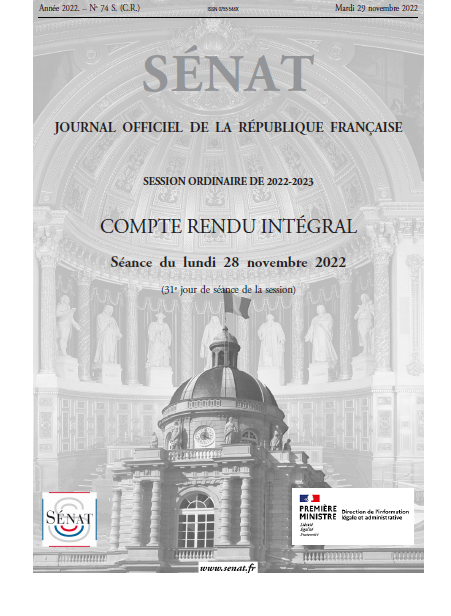
\includegraphics[width=0.6\textwidth]{images/JO.png}
    \caption{Image d'illustration d'un Journal officiel}
\end{figure}

\subsection{Historique et rôle des tables des matières dans les documents officiels du Sénat}

Les tables des matières sont des outils essentiels à la documentation des débats parlementaires du Sénat. Elles offrent une structure systématique qui permet de répertorier les interventions des sénateurs, les sujets débattus, ainsi que les actions législatives et non-législatives au sein des séances publiques et, depuis 2009, des commissions. Ces tables, produites annuellement, jouent un rôle crucial dans la transparence des travaux parlementaires en permettant aux chercheurs, aux journalistes et au grand public d'accéder facilement à l'information.\footcite{senat_tables_debats}

Le rôle des tables des matières a évolué au fil des décennies pour s'adapter aux besoins croissants de documentation et d'analyse. Elles ne se limitent plus à un simple index des interventions mais s'étendent à une classification détaillée des nominations, des dépôts législatifs, des questions, ainsi que des thèmes abordés lors des débats. Depuis avril 2009, elles incluent également les activités en commission, ce qui marque une étape importante dans l'exhaustivité des documents officiels.\footcite{senat_tables_debats}

\subsubsection{Présentation des différentes tables}

Les documents officiels du Sénat comprennent plusieurs types de tables des matières, chacune répondant à des besoins spécifiques en termes d'organisation et de consultation des données parlementaires :

\subsubsubsection{Table Nominative}

La Table nominative, ou Tome I, est un répertoire complet des activités individuelles des sénateurs pour une année donnée. Elle inclut un récapitulatif chronologique des nominations dans diverses commissions, des dépôts de propositions de loi, des interventions en séance publique, et, depuis 2009, des interventions en commission. Ce tome est un outil précieux pour l’analyse de la participation et des contributions des sénateurs. Il permet de retracer l’ensemble des actions parlementaires d’un sénateur sur une année et d’identifier ses domaines d’intervention.

\begin{figure}[H]
    \centering
    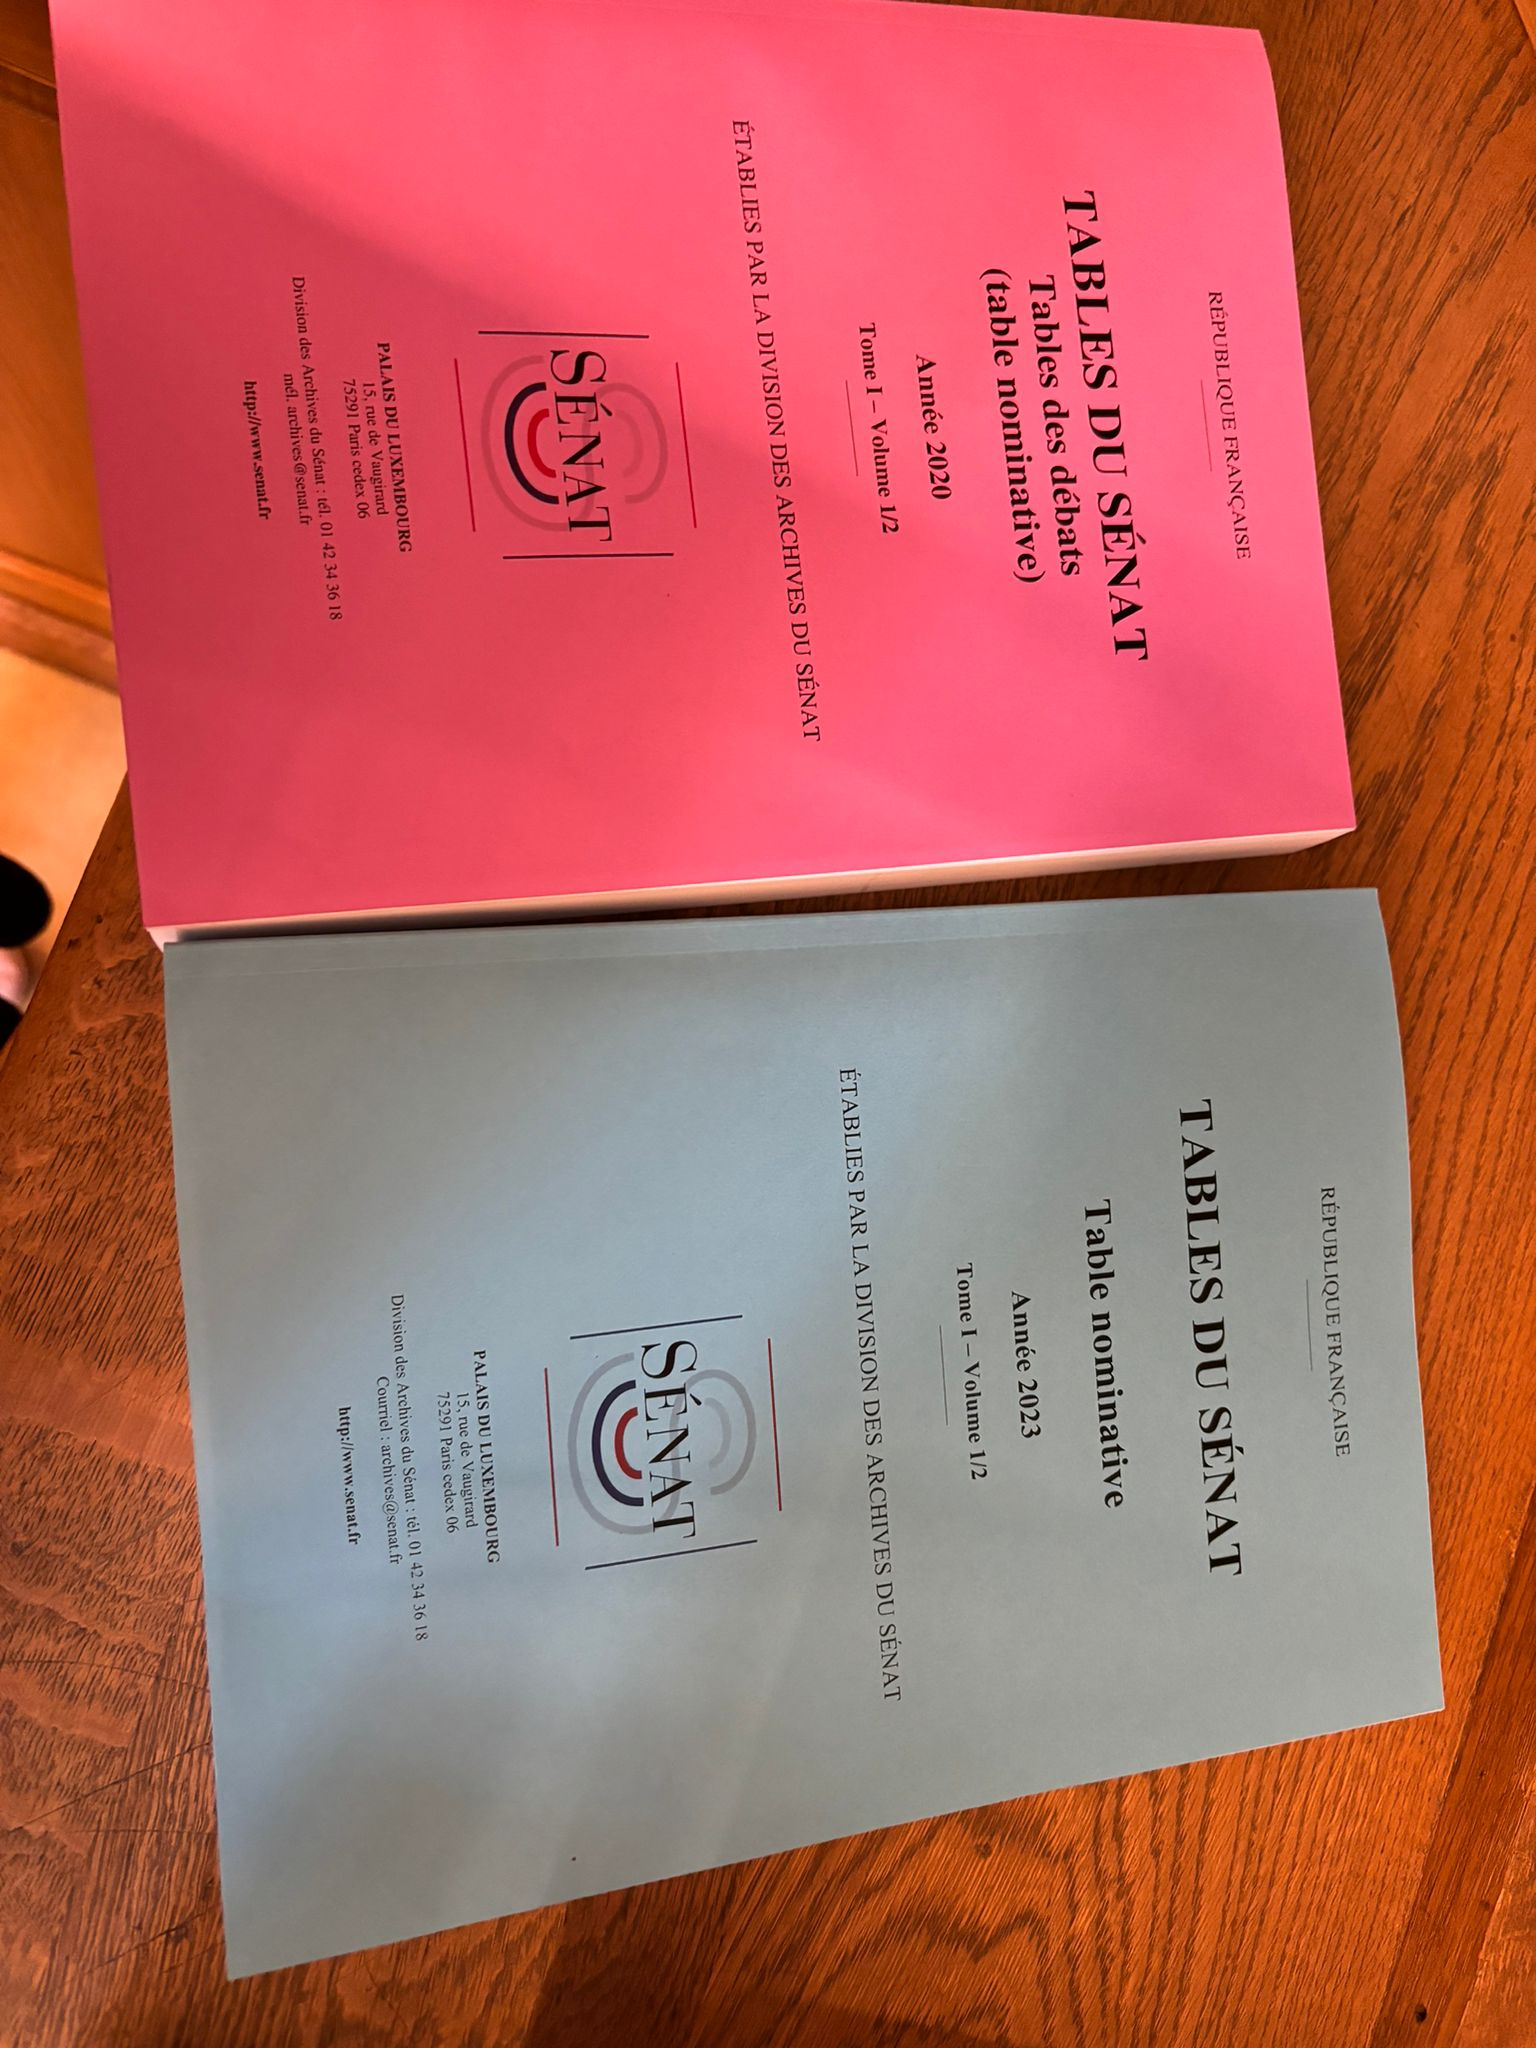
\includegraphics[angle=90, width=\textwidth]{images/tables nominatives.jpg}
    \caption{Photographie des tables nominatives du Sénat}
\end{figure}

Depuis 2017, deux innovations ont enrichi cette table : la mention des interventions, même lorsque la parole n'a pas été officiellement accordée, et la précision des sujets concernant les articles additionnels. Ces changements ont pour but de rendre compte de manière plus fidèle et complète des activités de chaque sénateur et sénatrice.

\subsubsubsection{Table Thématique}

La Table thématique, ou Tome II, organise les débats parlementaires selon les thèmes abordés au cours de l’année. Ce volume rassemble les propositions et projets de loi, les déclarations du gouvernement, les allocutions, et d’autres éléments comme les éloges funèbres et les motions de procédure. C'est un outil essentiel pour ceux qui cherchent à suivre l'évolution d'un sujet particulier sur plusieurs années, permettant de tracer les discussions législatives sur des thématiques spécifiques.

\begin{figure}[H]
    \centering
    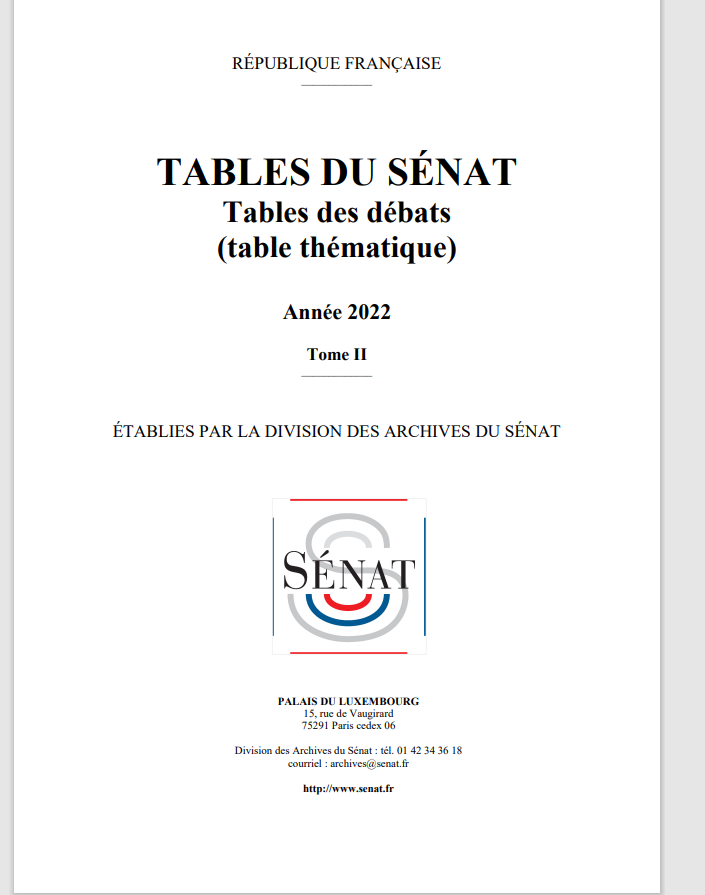
\includegraphics[width=0.6\textwidth]{images/tables thématiques .png}
    \caption{Capture d'écran des tables thématiques du Sénat\protect\footnote{Sources:https://www.senat.fr/les-tables-des-debats.html}}
\end{figure}

\subsubsubsection{Composition et activités des organes du Sénat (Tome III)}
Le troisième volume se concentre sur la composition et les activités des différents organes du Sénat. Il contient des listes détaillées des sénateurs, la composition des \gls{groupes_politiques}, du \gls{bureau_senat}, des \gls{commissions_permanentes} et \gls{commissions_temporaires}, ainsi que des \gls{delegations_structures}. Ce volume documente aussi les \gls{changements_organes}, la \gls{cour_justice_republique}, les \gls{organismes_extra_parlementaires}, les \gls{petitions}, et les \gls{rapports} remis au Parlement. Ce tome est basé sur les informations publiées dans le \textit{Journal officiel Lois et décrets}\footnote{Disponible sur: \url{https://www.legifrance.gouv.fr/jorf/jo}}, garantissant un suivi rigoureux et précis de l’activité parlementaire.
\begin{figure}
    \centering
    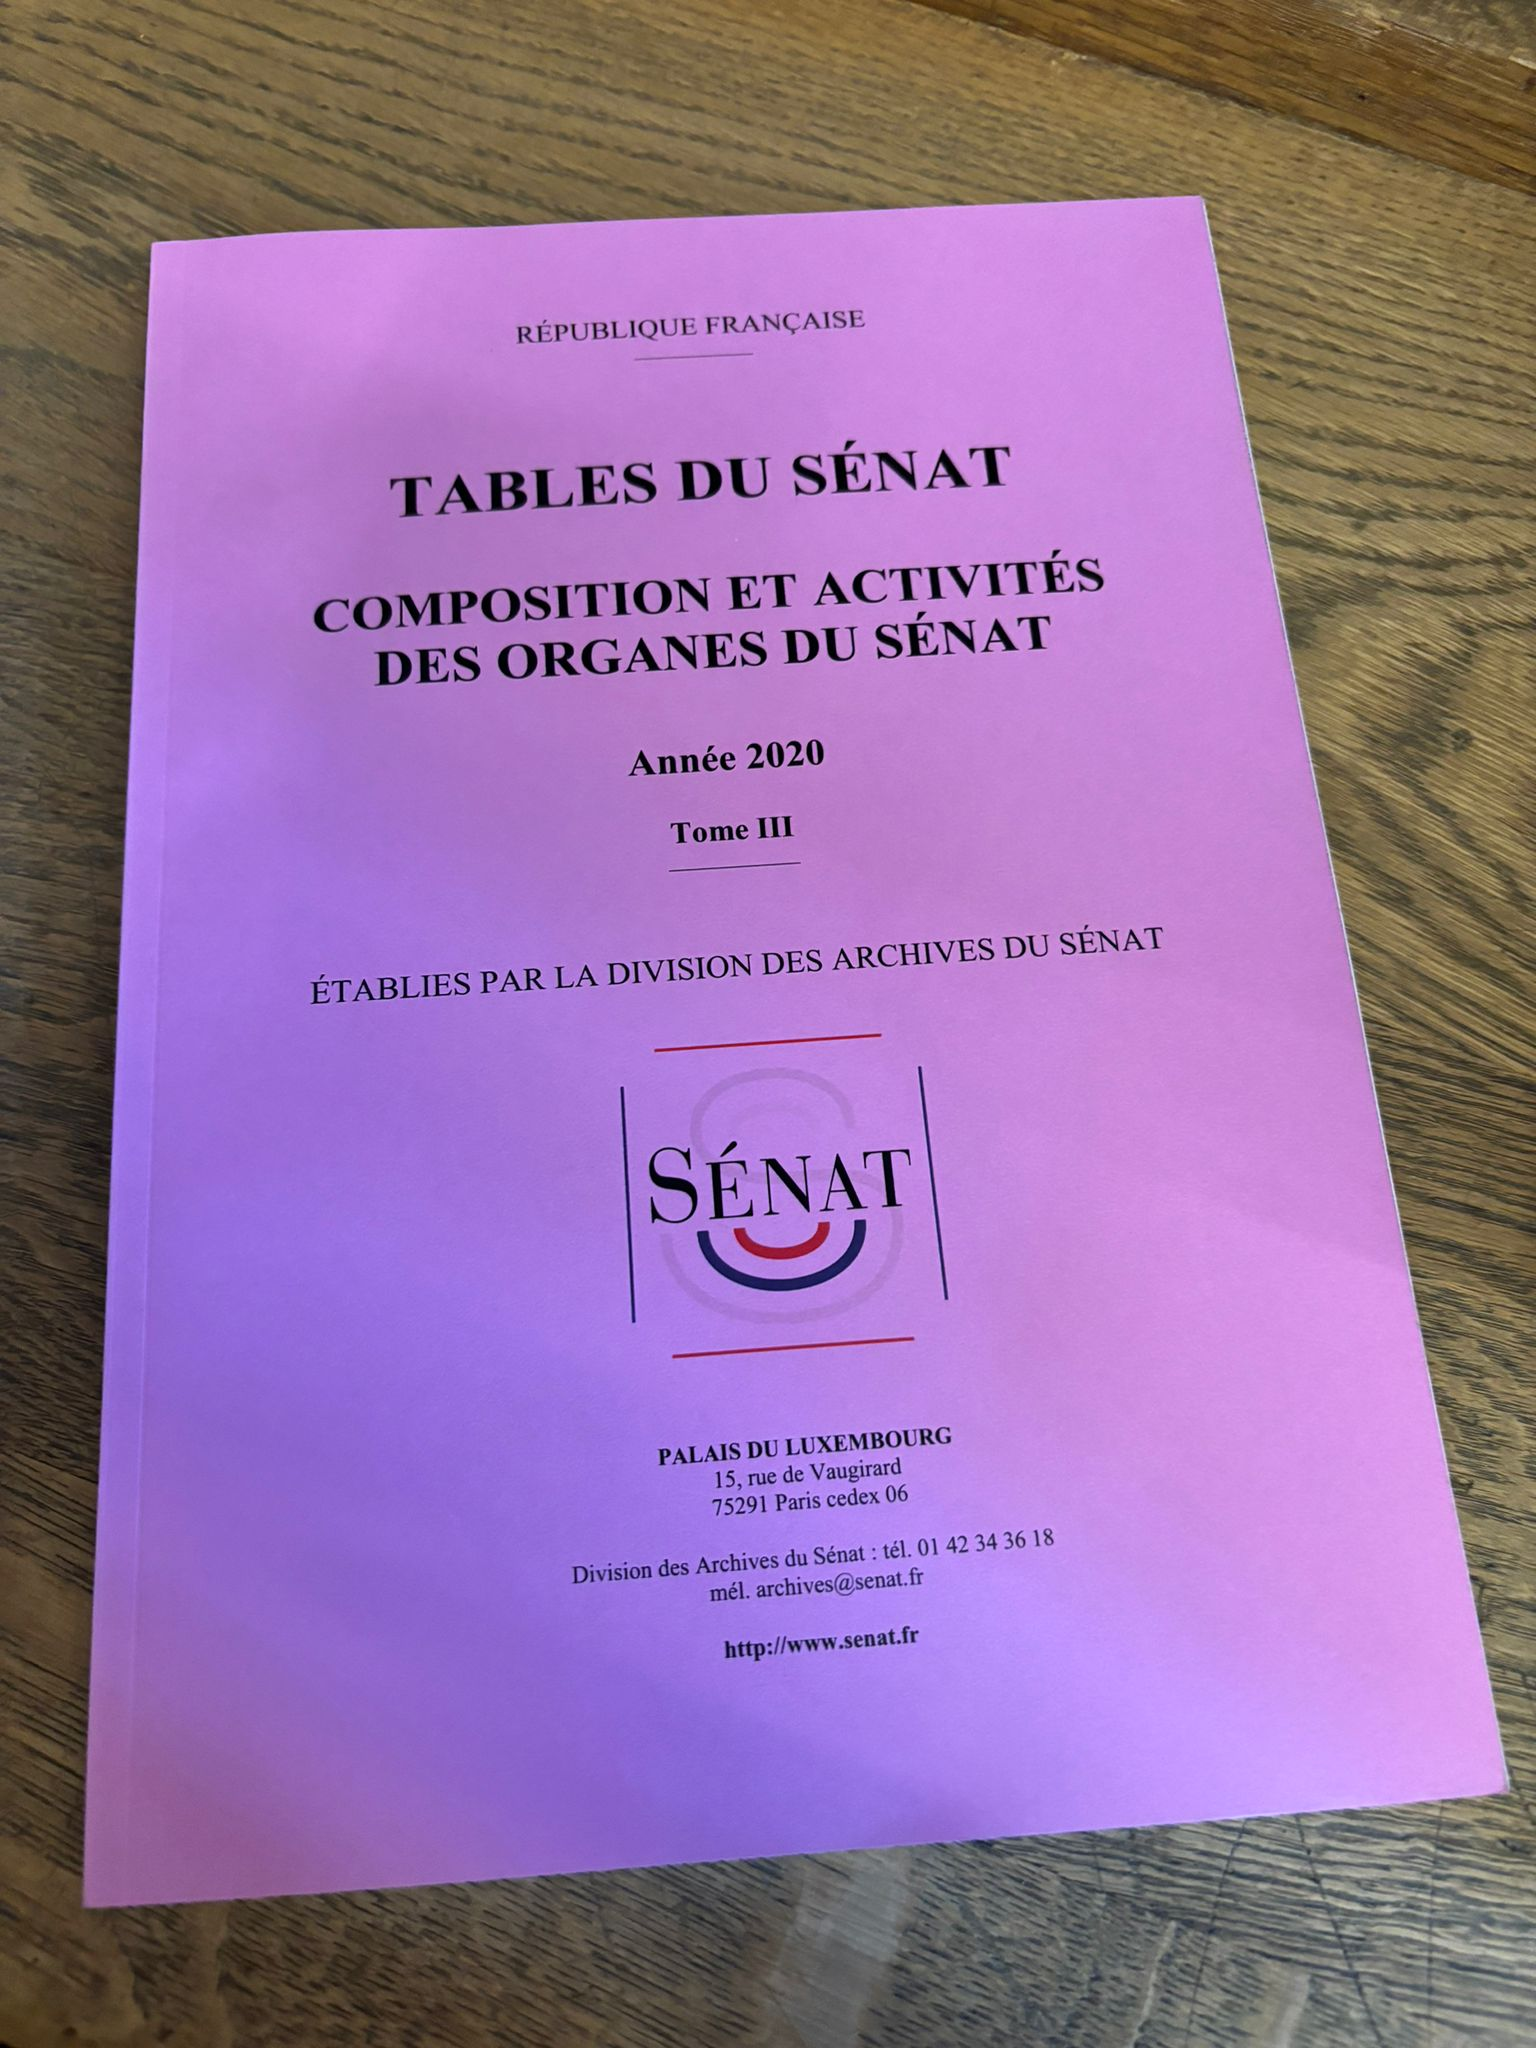
\includegraphics[width=0.5\linewidth]{images/tables3.jpg}
    \caption{Tables du Sénat- Tome III}
\end{figure}
Ces trois volumes, constituant les Tables des débats du Sénat, sont des ressources essentielles pour toute personne souhaitant suivre, analyser, ou étudier les travaux du Sénat français. Ces différentes tables constituent des outils indispensables pour la navigation et la recherche dans les archives parlementaires. Elles garantissent non seulement la transparence du processus législatif mais aussi la préservation de la mémoire institutionnelle du Sénat.

\section{L'importance des tables pour comprendre le fonctionnement de la séance publique}
\subsection{Intervenants de séance publique}

Les interventions en séance publique sont documentées de deux façons : par jour de séance et par texte de loi discuté. La présentation par jour de séance regroupe toutes les interventions de l’orateur pour une journée donnée, incluant à la fois les discussions sur les textes de loi et d'autres types de débats. En ce qui concerne la présentation par texte de loi, elle rassemble toutes les interventions de l’orateur relatives à un texte de loi spécifique. De plus, les projets de loi déposés par les ministres, ainsi que l’ensemble de leurs interventions en séance publique, sont également répertoriés dans la Table nominative.

L’équipe chargée des archives joue un rôle central dans ce processus en intervenant pour analyser les Journaux Officiels (JO). Grâce à leur travail minutieux, les données sont extraites, organisées et synthétisées afin d'être intégrées dans ces tables du Sénat. Leur intervention est essentielle pour garantir la précision et l’exhaustivité des informations présentées, permettant ainsi aux utilisateurs de naviguer facilement à travers les multiples débats et interventions. Cette contribution garantit que les tables du Sénat reflètent fidèlement les activités parlementaires et facilitent la recherche et l’analyse des débats par thème ou par sénateur.

\begin{figure}[H]
    \centering
    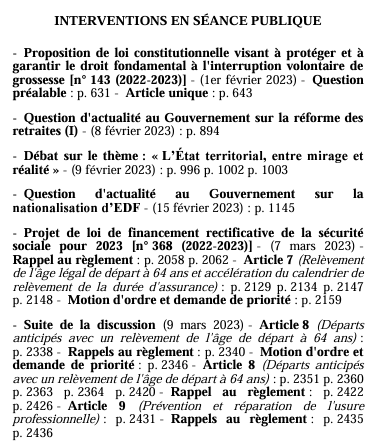
\includegraphics[width=0.5\linewidth]{images/Interventions Séances Publiques.png}
    \caption{Illustration d'intervention des Séances Publiques dans les Tables Nominatives\protect\footnote{source : \url{https://www.senat.fr/les-tables-des-debats.html}}}
\end{figure}

\subsection{Projet de loi et proposition de loi}

Un projet de loi est un texte législatif proposé par le gouvernement pour être examiné et adopté par le Parlement. Il émane généralement de l'exécutif et traduit la volonté politique du gouvernement de mettre en place une nouvelle législation ou de modifier des lois existantes. Les projets de loi sont souvent rédigés par les ministères concernés et soumis au Parlement après avoir été approuvés en Conseil des ministres. Une fois déposés, ils sont discutés en séance publique, où les sénateurs et les députés peuvent proposer des amendements avant de procéder au vote.

En revanche, une proposition de loi est un texte législatif proposé par un ou plusieurs parlementaires, sans l'intervention directe du gouvernement. Elle permet aux membres du Parlement d'initier des réformes législatives ou d'aborder des questions d'intérêt public qui ne sont pas nécessairement prioritaires pour l'exécutif. Comme les projets de loi, les propositions de loi sont examinées en séance publique, où elles peuvent être amendées et votées. Si elles sont adoptées par les deux chambres du Parlement, elles peuvent devenir des lois à part entière, au même titre que les projets de loi.

\section{Le processus de création des métadonnées de l’équipe d’archivistes}

\subsection{Équipe d'analyse et de bornage du JO aux archives}
Dans le processus d'élaboration des Tables du Sénat, l'analyse et le \gls{bornage} des JO sont fait par l'équipe de six personnes aux archives du Sénat.

\begin{figure}[H]
    \centering
    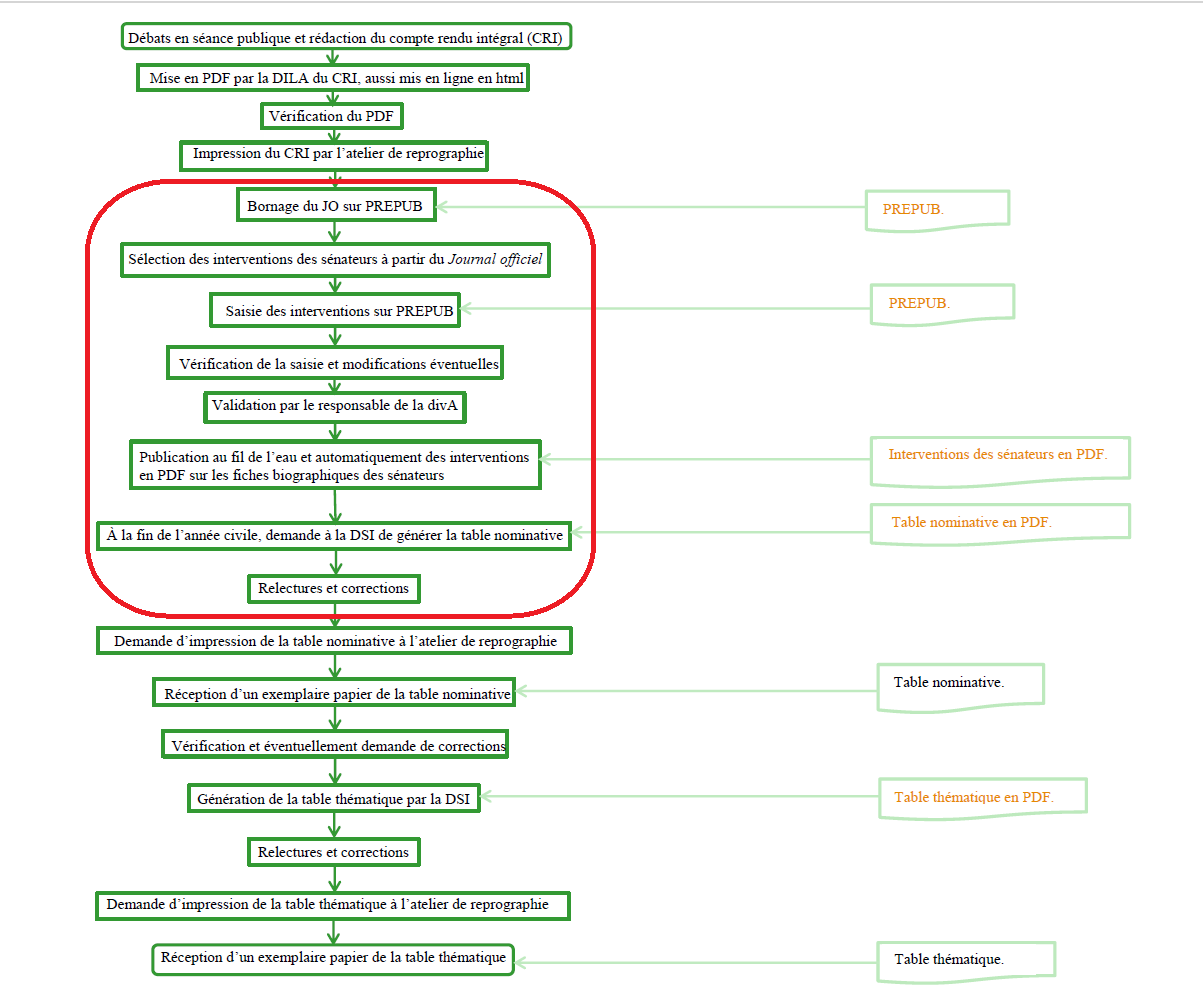
\includegraphics[width=1\textwidth]{images/Schéma de création les tables nominatives et thématiques.png}
    \caption{Schéma d'illustration des étapes de création d’instruments de recherche : les tables nominatives et thématiques \footcite{Lesdirectiondelabiblioetdesarchives}}
\end{figure}

Tout d'abord, les assistantes de gestion et de direction (ADG), Mme Line Zeppa, Mme Frédérique Pawloff et Mme Nathalie Palacios, s'occupent du traitement initial des Journaux officiels. Elles sont chargées de saisir les analyses de Madame Ghislaine Laumonerie concernant les projets de loi (PPL et PJL), ainsi que les interventions liées aux débats thématiques et aux questions diverses. En outre, elles effectuent les corrections demandées par M.Franck Pariguet et Mme Ghislaine Laumonerie. Cette étape constitue la base du processus de traitement des informations des JO.

Une fois le travail des ADG terminé, Mme Ghislaine Laumonerie, en tant qu’administratrice-adjointe, vérifie et valide les JO dans le système \gls{Prepub}. Elle est responsable de la sélection des interventions pertinentes à inclure dans les Tables du Sénat, ainsi que de la vérification finale des JO pour garantir leur exactitude avant de passer aux étapes suivantes. Elle gère également l’archivage et l’élimination des JO selon des délais fixés.

M.Franck Pariguet, en tant qu'assistant de gestion et de direction, poursuit en relisant les écrans de validation imprimés par les ADG. Il s’assure que la pagination est correcte, recherche les erreurs et garantit que toutes les données sont saisies de manière précise. Lorsqu'il détecte des erreurs ou des omissions, il demande aux ADG de procéder aux corrections nécessaires pour garantir l'intégrité des données.

Enfin, Mme Stéphanie Sanna, en tant qu’administratrice-adjointe, réalise la dernière vérification. Son rôle est de s'assurer que toutes les modifications additionnelles ont été correctement traitées. Une fois cette étape terminée, elle transmet la version papier du JO à Mme Ghislaine Laumonerie pour la validation finale dans le cadre du processus.

\subsection{Bornage et saisie des Journaux Officiels.}

\begin{figure}[H]
    \centering
    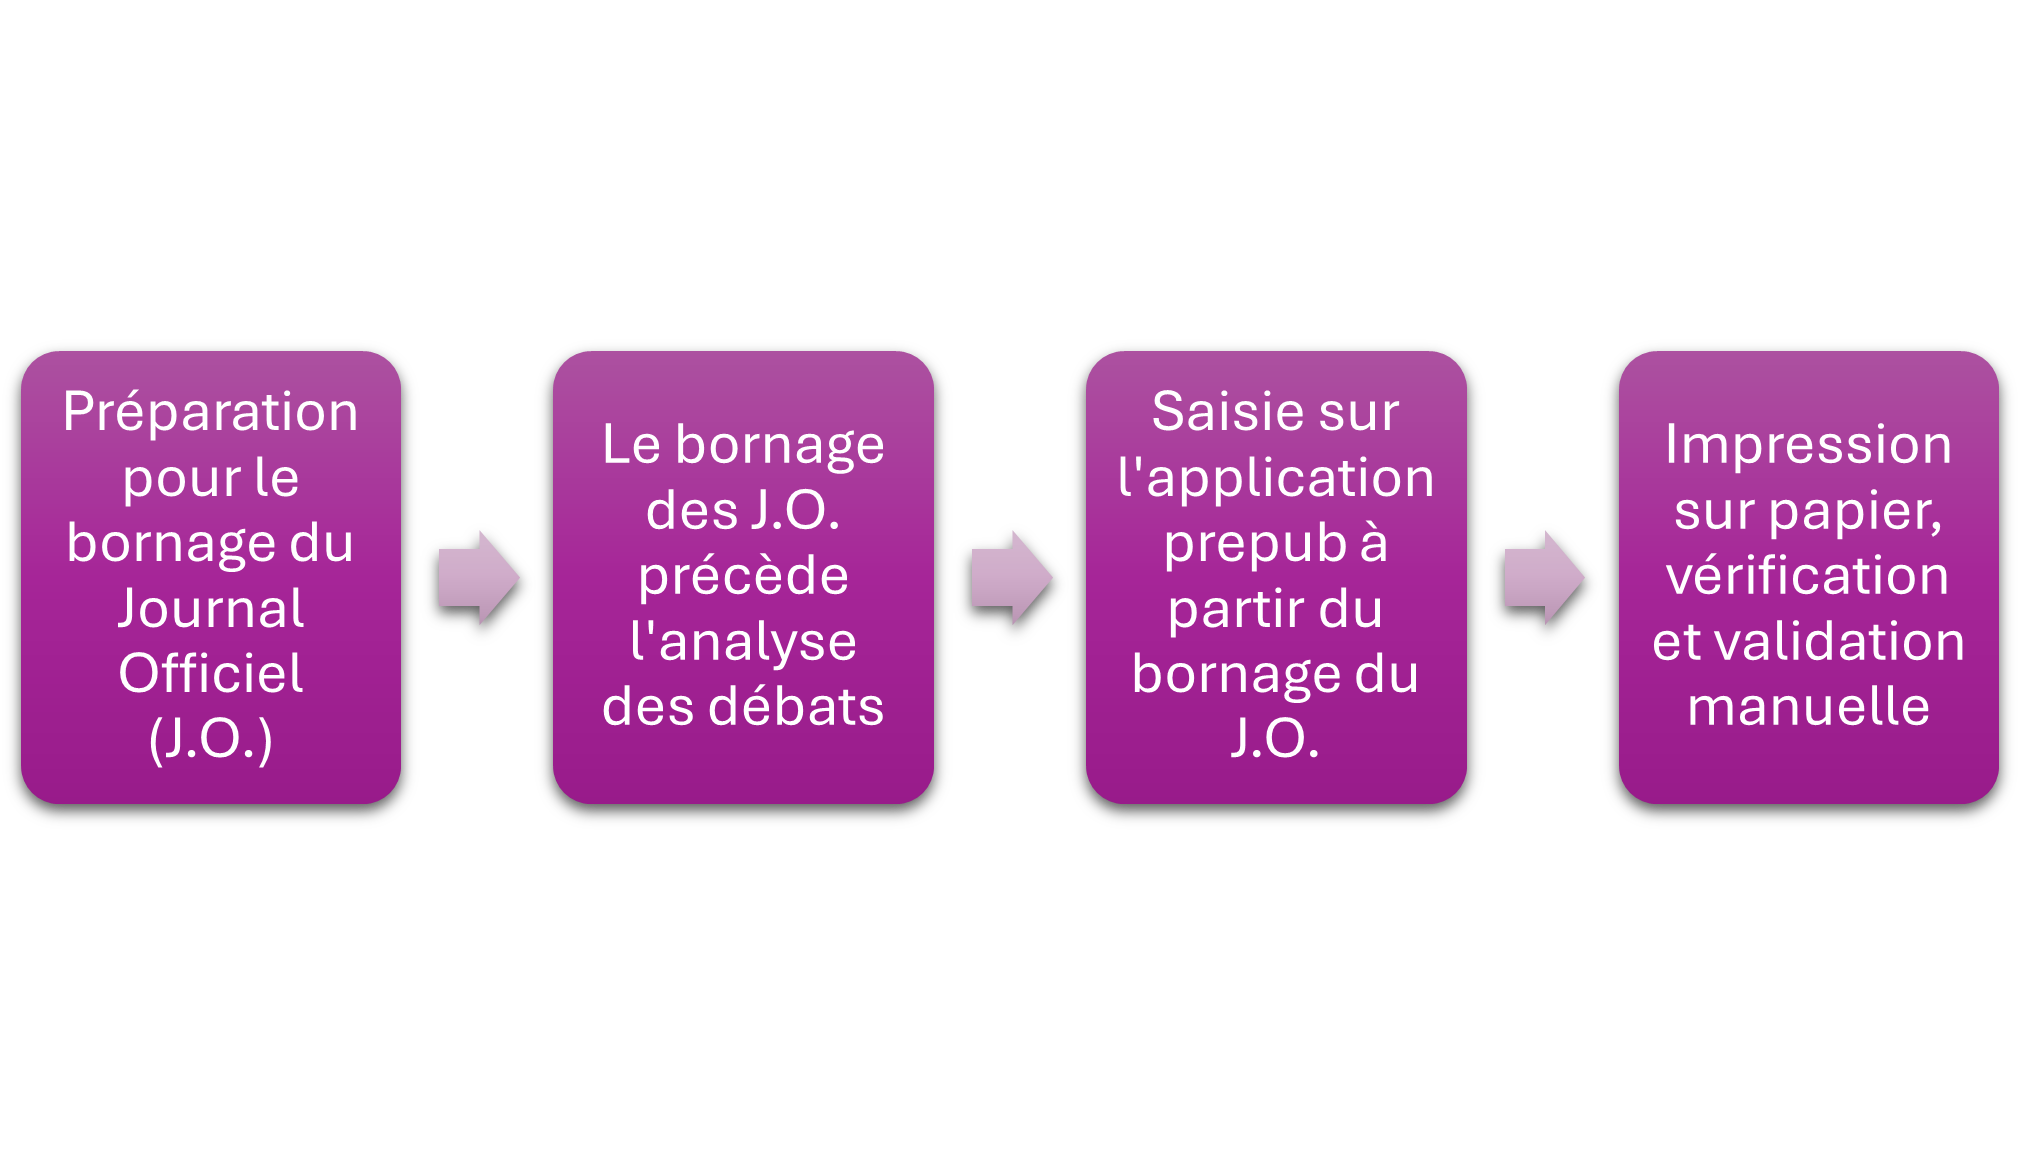
\includegraphics{images/Schéma Bornage Prepub.png}
    \caption{Schéma d'illustration des étapes du bornage dans Prepub}
\end{figure}

\paragraph{Préparation des JO papier}

Les JO papier sont annotés dès leur réception. La date de réception est inscrite sur la page de couverture, et des crayons de couleur sont utilisés pour identifier les sections importantes qui nécessitent une analyse approfondie.

\paragraph{Connexion à l'application Prepub}
%%%Prepub est un logiciel d'archivage interne au Sénat, il sert à la fois au moment du bornage, du choix des interventions et de leur saisir, ainsi qu'au moment de la validation finale du JO traité. 

L'utilisation de l'application \gls{Prepub} qui est un logiciel d'archivage interne au Sénat, il sert à la fois au moment du bornage, du choix des interventions et de leur saisir, ainsi qu'au moment de la validation finale du JO traité, suit la préparation initiale du JO papier. Cette application, spécifique à la division des Archives du Sénat, permet le bornage numérique des Journaux Officiels, facilitant la navigation et l'utilisation des menus déroulants pour marquer les sections préalablement soulignées.

\paragraph{Le bornage proprement dit};

Le bornage implique plusieurs sous-étapes :

\begin{itemize}
    \item \textbf{Bornage des Textes de Lois}: L'application Prepub est utilisée pour naviguer à travers le sommaire et délimiter les textes de loi, marquant les débuts et les fins des discussions.

\begin{figure}[H]
    \centering
    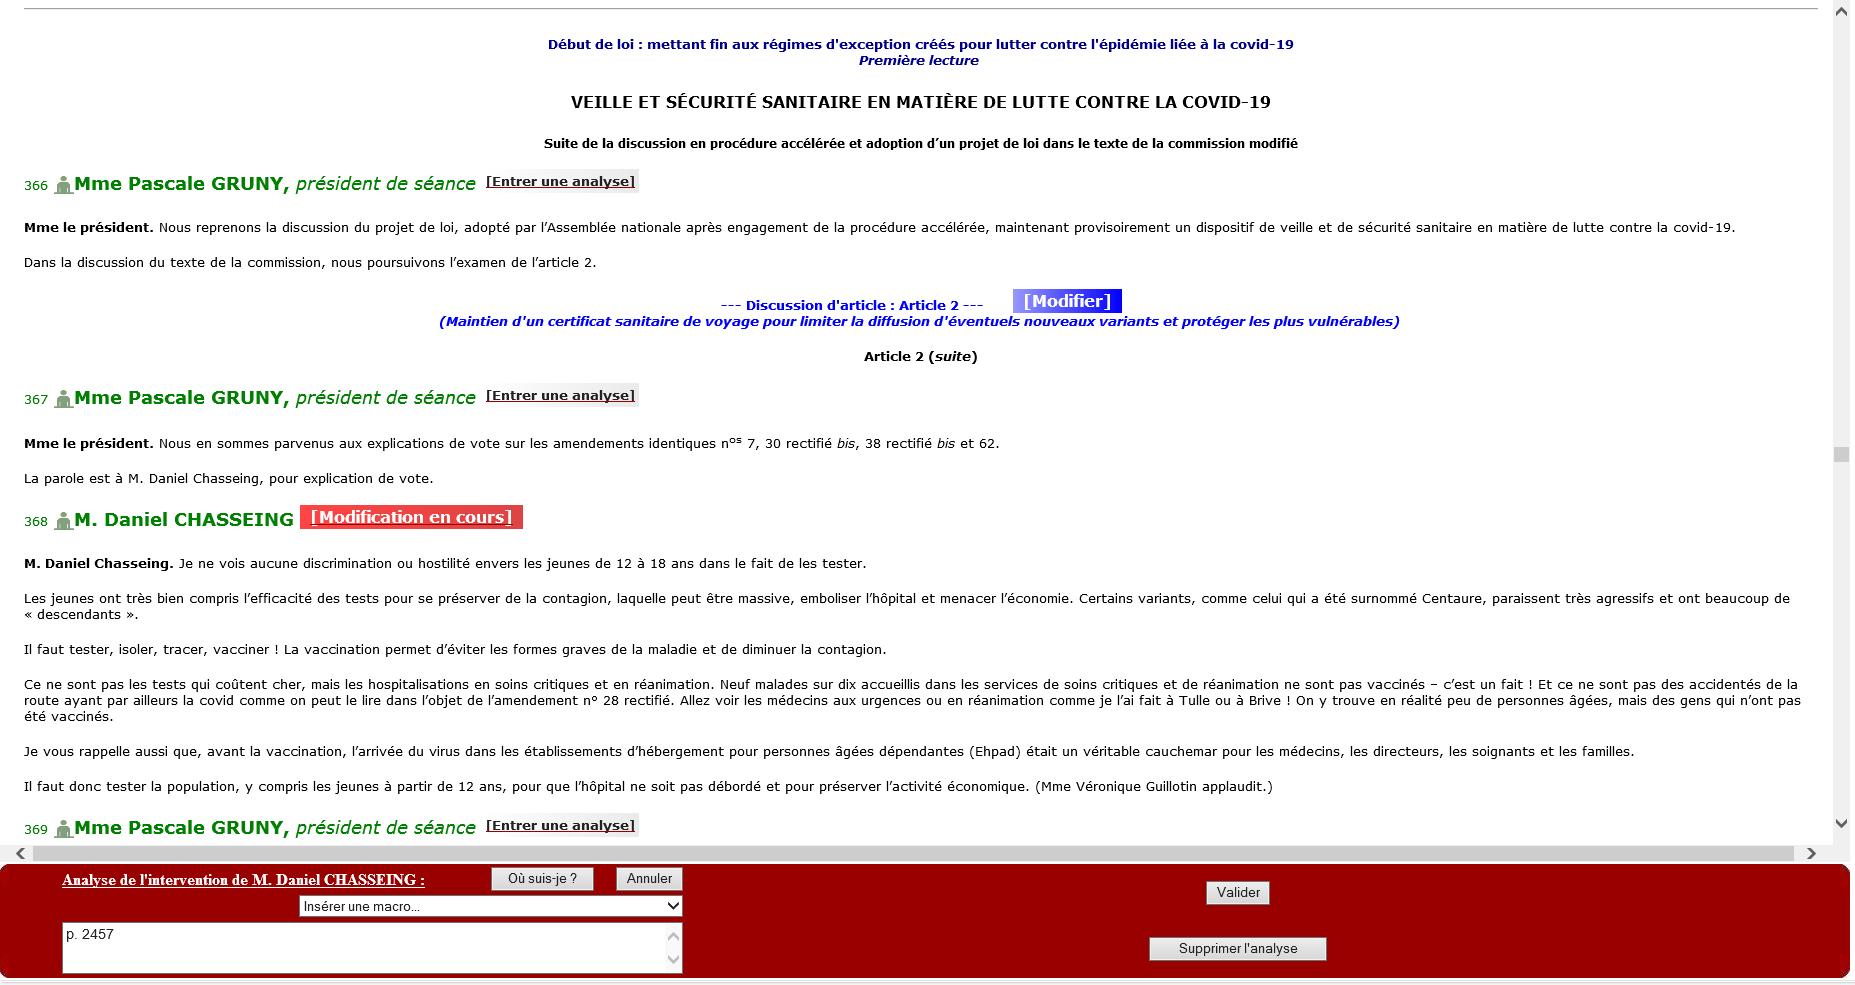
\includegraphics[width=1\linewidth]{images/article.png}
    \caption{Capture d'écran d'application de Prepub}
\end{figure}
    
    \item \textbf{Bornage de textes législatifs hors lois}: Les interventions non liées directement aux textes de loi, comme les allocutions, sont également bornées en utilisant des subdivisions appropriées dans l'application.
\end{itemize}

\paragraph{Vérification et impression}

Une fois le bornage terminé, une vérification est effectuée pour valider l'exactitude des informations. Le processus se conclut par l'impression du bornage pour une relecture, ce qui comprend la date du bornage et les initiales de la personne ayant réalisé le travail, assurant ainsi une traçabilité et une validation finale avant l'enregistrement officiel des données. 

Ces étapes détaillées illustrent l'engagement et la rigueur de l'équipe d'archivistes dans la gestion des métadonnées du Journal Officiel, garantissant une documentation précise et accessible des activités parlementaires.

\subsection{Processus actuel de collecte et de gestion des métadonnées}

L'équipe d'archivage travaille en étroite collaboration avec la Direction du Compte Rendu (DCR) et la Direction des Systèmes d'Information (DSI) pour optimiser la gestion des métadonnées. Les étapes clés de ce processus comprennent les processus suivants:

\begin{figure}[H]
    \centering
    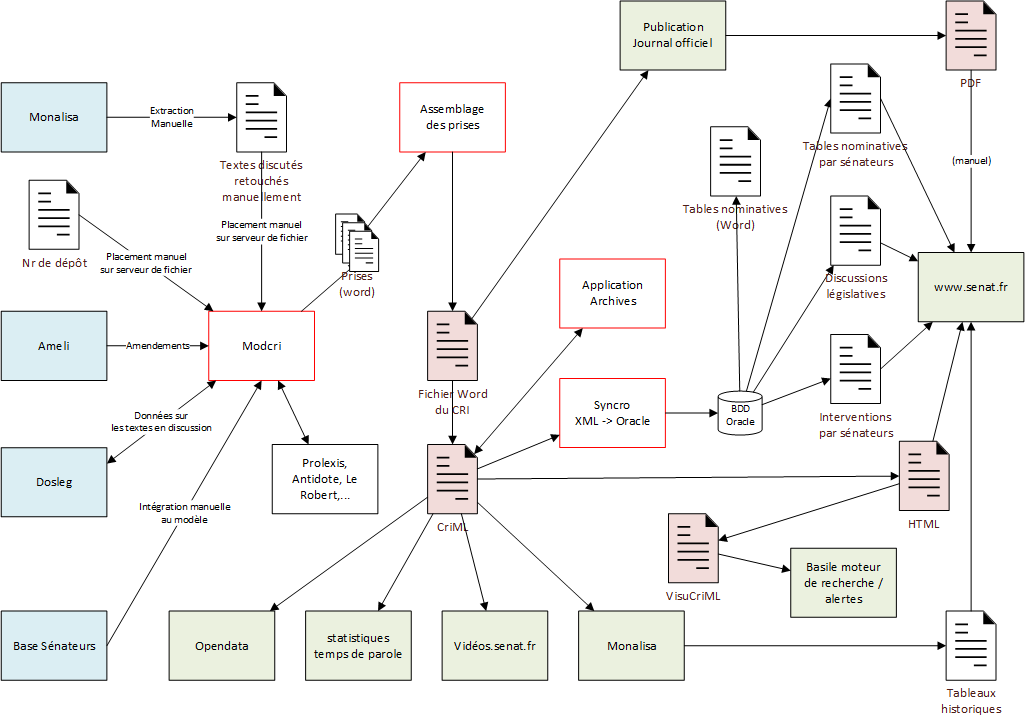
\includegraphics[width=1\linewidth]{images/cri.png}
    \caption{Schéma SI lien avec CRI, fournit par les archivistes du Sénat}
\end{figure}


\subsubsection{Initialisation et Conversion des Documents}

Les comptes rendus sont d'abord rédigés en format WORD (.DOCX) par la DCR avant d'être convertis en format .DOC pour transmission à la \gls{DILA}, une étape automatisée pour assurer l'uniformité et la compatibilité des fichiers. Ces documents sont ensuite transformés de .\gls{XML} en .\gls{HTML} pour une publication en ligne, suivie d'une conversion finale en format \gls{PDF} validée par la \gls{DILA} en vue d’une diffusion plus large, y compris sur Légifrance.\footcite{VadeMecum}

\subsubsection{Gestion Documentaire et Vérifications}

La DCR, en plus des conversions de format, intègre des macros dans le modèle WORD utilisées pour insérer automatiquement des phrases types fréquemment utilisées, facilitant ainsi la standardisation des procédures telles que les prises de parole et les mises aux voix. Des vérifications supplémentaires sont effectuées par des membres de la DCR, comme Guillaume JANDOT, pour s'assurer de la précision des comptes rendus avant leur publication dans l’application Prepub.\footcite{VadeMecum}

\subsubsection{Publication et Accès aux Données}

- Les fichiers finalisés destinés à l'Open Data, c'est à dire à la publication "ouverte" sur le site du Sénat, sont exportés depuis \gls{Prepub} en format .\gls{XML}, avec leurs métadonnées associées, vers les serveurs du site senat.fr\footnote{Fichiers .\gls{XML} et .\gls{SQL} accessibles ici : https://data.senat.fr/la-base-comptes-rendus/} permettant une accessibilité et une réutilisation optimales des données pour tous. 
- Les Tables des séances, tout comme la Table nominative, sont quant à elles générées à partir de l'ensemble des informations contenus dans ces fichiers source .\gls{XML}/.\gls{SQL} et rationalisent les entrées listées dans ces bases de données grâce au logiciel \gls{Prepub} afin de publier son contenu sous format .\gls{PDF} dans le JO électronique.

\subsubsection{Assemblage et Publication des Fichiers}

Chaque compte rendu, composé initialement de plusieurs fichiers .WORD rédigés par différents auteurs, est assemblé pour former un document \gls{XML} unique par séance. En collaboration avec la DSI, des schémas explicatifs du système informatique lié au CRI ont été élaborés pour illustrer le flux de données et leur traitement.

Ces étapes illustrent un processus complexe et intégré de gestion des métadonnées qui non seulement permet un archivage précis des activités parlementaires mais assure également une transparence et une accessibilité accrues pour le public et les chercheurs. Les défis liés à ce processus, notamment la gestion manuelle et la complexité des formats, nécessitent une vigilance continue pour maintenir l'intégrité et la précision des archives.
\section{Analyse des limitations et des défis du processus manuel}

Le processus manuel de gestion des métadonnées du \gls{JO} par l'équipe d'archivistes présente plusieurs défis significatifs liés à la consommation de ressources humaines et au temps nécessaire pour assurer la précision des archives :

\subsubsection{Intensité de la main-d'œuvre}

La gestion manuelle des métadonnées du \gls{JO} nécessite l'implication d'une équipe de six personnes, qui doivent lire et relire chaque édition pour en assurer l'exactitude. Cette approche est extrêmement exigeante en termes de ressources humaines, chaque membre de l'équipe devant examiner minutieusement les documents pour identifier et corriger les erreurs potentielles. Cette intensité de la main-d'œuvre rend le processus non seulement coûteux mais aussi sujet à des risques d'erreur accrus du fait de la fatigue et des erreurs humaines.

\subsubsection{Consommation excessive de temps}

Le processus requiert que chaque \gls{JO} soit passé en revue plusieurs fois pour s'assurer que toutes les métadonnées sont correctement bornées et enregistrées. Cette révision multiple est chronophage, retardant potentiellement la disponibilité des informations pour les utilisateurs finaux et impactant l'efficacité globale de l'archivage. La nécessité de multiples lectures et de vérifications augmente le risque d'erreurs humaines dans le bornage et la saisie des métadonnées. Chaque erreur nécessite des révisions et des corrections supplémentaires, augmentant encore le temps consacré à chaque \gls{JO} et exacerbant la charge de travail de l'équipe.

\subsubsection{Dépendance à la précision humaine}

La dépendance du processus à la précision humaine dans la lecture et la saisie des données peut entraîner des incohérences et des lacunes dans les archives. Cette situation est particulièrement problématique dans un contexte où les erreurs peuvent compromettre l'intégrité des données historiques et législatives, essentielles pour les recherches et les références futures.

\subsubsection{Une mise à l’échelle limitée}

La mise à l’échelle du processus est limitée par la capacité humaine à gérer un volume toujours croissant de données. Sans possibilité d'augmenter de manière flexible le nombre de membres de l'équipe ou d'intégrer des solutions techniques avancées, il est difficile de répondre efficacement aux besoins changeants de gestion des archives.

Ces limitations mettent en évidence la nécessité d'adopter des méthodes plus automatisées et moins dépendantes de l'intervention humaine intensive. L'automatisation pourrait réduire le nombre de lectures nécessaires, diminuer le risque d'erreurs, et améliorer la rapidité de traitement des \textit{Journaux Officiels}, tout en conservant les ressources précieuses de l'équipe d'archivistes.

 
	\part{Études de corpus et tâches d'automatisation }
	
	\chapter*{Deuxième Partie : Le corpus et données : l’exemple de l’année 2022}
\setcounter{chapter}{2}  % Đặt lại số chương thành 2
% images, schema, Lucidchart pour faire des schémas

\section{Présentation du corpus : Journaux Officiels 2022}

Au cœur de cette étude se trouve les Journaux Officiels (JO) de l'année 2022, qui sont comptes rendu intégraux des séances plénière en 2022. Ce corpus constitué de 86 fichiers totalisant 8485 pages.

Le texte brut des comptes rendus est disponible au format WORD, mais après publication, les fichiers sont accessibles à la fois en \gls{PDF} et en une seule page \gls{HTML} depuis le site officiel du Sénat : \url{https://www.senat.fr/seances/seances.html}.
De plus, une version \gls{XML} de ces documents est transmise pour l'intégration dans la base de données officielle du Sénat, et est accessible directement depuis leur site web : \url{https://data.senat.fr/la-base-comptes-rendus/}.
Au-delà de leur diversité de formats et de mise en page, ces documents partagent tous un même contenu. Après avoir lu différents formats pour identifier les détails à extraire, ainsi que la structure propre à chaque format, il a été conclu que la version du document au format \gls{PDF} serait principalement utilisée dans le processus d'extraction automatique. En effet, ce choix repose sur l'exhaustivité des détails et leur intégration dans un texte facile à analyser de manière automatique. Concernant le format WORD, la forme et la structure ne sont pas adaptées au traitement automatique, car le contenu n'est pas divisé en colonnes, la taille et la police des caractères ne sont pas toujours correctement configurées, enfin, les numéros de page ne sont pas marqués.
Par ailleurs, les fichiers \gls{HTML} et \gls{XML} ne sont pas structurés en colonnes et ne comportent pas de numéros de page. Cependant, la lecture et l'enregistrement des balises de données au format \gls{XML} peuvent faciliter l'intégration des informations extraites dans des bases de données ou des systèmes de pré-publication après extraction.

\subsection{Pourquoi avoir choisi d’expérimenter sur les documents de 2022}

Le choix de l'année 2022, année faisant suite à deux ans marqués par la pandémie de Covid-19, s'explique par le fait que les sujets discutés reprennent alors un cours plus normal, se détachant des questions sanitaires pour mieux se recentrer sur des enjeux de long terme au cœur des débats.

De plus, après avoir échangé avec le directeur des archives, Jean-Marc Tichi, et l'équipe des archives, le choix de l'année 2022 s'explique également par le fait qu'il s'agit d'une année récente pour laquelle Mme Ghislaine Laumonerie a encore conservé quelques Journaux Officiels au format papier, car ceux des années antérieures n'ont plus tous été gardé physiquement. Cela nous permet donc de montrer clairement les annotations manuscrites sur les Journaux Officiels et de mieux comprendre les détails du processus de travail en équipe. Elle précise que l'année 2023 ne pouvait pas être utilisée, car elle n'était pas encore entièrement traitée au début du stage en avril 2024. Il était important d'éviter toute interférence avec le travail en cours sur les Journaux Officiels de 2023 et l'élaboration de la Table nominative de 2023.


\section{Étude des Corpus}

Nous avons effectué une lecture rapide du document afin de localiser des éléments clés comme la table des matières, les titres des sections et sous-sections, afin de mieux comprendre la structure générale du document ainsi que ses sections principales, et mieux saisir l'organisation du contenu pour accéder rapidement aux informations essentielles. Après avoir lu plusieurs exemples, nous avons une vision claire du format commun et de la structure de tous les JOs. Cette approche nous a permis d'identifier des informations cruciales, notamment le nom des intervenants, les dates, les textes de loi, les sujets de discussions, etc...

\subsection{Structure générale d'un compte rendu}
La structure générale d'un fichier de compte rendu comprend plusieurs éléments. La page de titre contient : le titre, la date de la séance, la date de publication du \gls{JO} ainsi qu'une image du Sénat sur la couverture. Le contenu principal est organisé avec, sur chaque page, un en-tête comprenant le titre, la date et la session. Les parties principales incluent un sommaire qui liste les sujets abordés et les intervenants, un compte rendu intégral des débats, et des annexes (facultatif).

Les documents parlementaires ou les rapports officiels sont divisés en plusieurs colonnes pour organiser le texte. Dans le cas de ce document, le contenu est souvent disposé en deux colonnes principales. Cela permet de gagner de la place au moment de l'impression. Le document est structuré en fonction des séances ou des jours de réunion, avec des titres clairs comme "Séance du [date]" pour indiquer la date de la séance. Cela permet de retrouver clairement les informations relatives à une séance spécifique. Cependant, la mise en signet se poursuivra de session en session. Les numéros de page sont marqués de la première séance à la dernière séance de l'année et le marquage des pages sera repris à la première séance de l'année suivante.

\subsection{Éléments de contenu principaux dans le texte}

\begin{figure}[H]
    \centering
    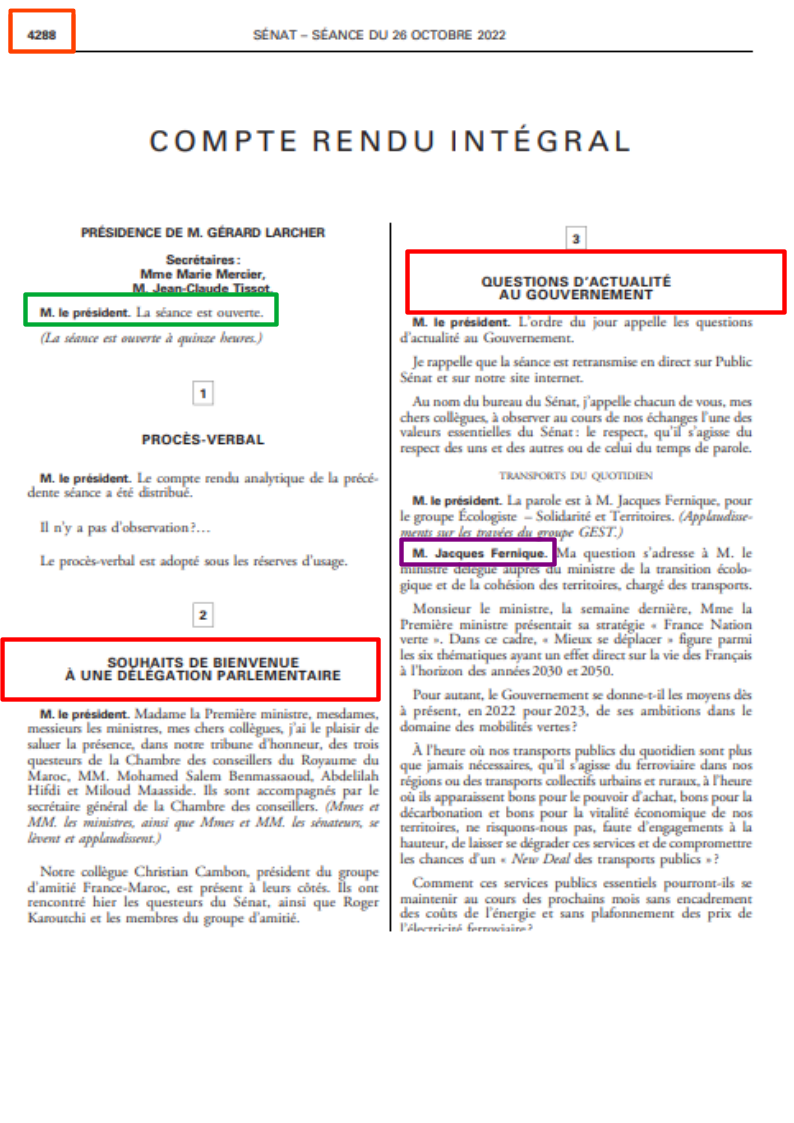
\includegraphics[width=0.7\textwidth]
    {images/structure.png}
    \caption{Capture de JO du 26 octobre 2022}
\end{figure}

\paragraph{Noms des intervenants} Les noms apparaissent souvent sous la forme "M. [Nom]" ou "Mme [Nom]" et sont en gras ou clairement distingués pour être facilement identifiables. Après le nom suit la prise de parole ou l’échange de cet intervenant.

\paragraph{Sujets de discussion} Dans chaque séance, les sujets principaux sont clairement présentés à travers des titres écrits en majuscules et centrés sur la page en dessous du numéro du titre encadré . Par exemple, des sections comme "SOUHAITS DE BIENVENUE À UNE DÉLÉGATION PARLEMENTAIRE" ou "QUESTIONS D’ACTUALITÉ AU GOUVERNEMENT" sont toujours bien visibles, permettant aux lecteurs d'identifier rapidement les différentes parties du débat. Cette présentation structurée aide à naviguer efficacement dans les discussions et à suivre le déroulement des séances parlementaires.

\paragraph{Numéro de pages} Le numéro de pages est systématiquement placé en tête de chaque page dans les documents officiels, facilitant ainsi la navigation et la référence. La numérotation est continue à partir de la première séance de l'année jusqu'à la dernière, sans interruption, ce qui permet de suivre les débats et les décisions de manière cohérente tout au long de l'année législative. Ce système assure une traçabilité et une transparence dans l'organisation des séances.

\paragraph{Subdivision du texte} Les sections sont divisées en petits paragraphes, souvent marqués par des titres ou des numéros d’articles ou d’amendements (par exemple, "Article 1er").

\paragraph{Nature de texte} La nature de textes de loi qui écrit en majuscule et dessus de textes de lois

\begin{figure}[H]
    \centering
    \includegraphics[width=0.45\textwidth]{images/Article.png}
    \caption{Capture de JO du 26 octobre 2022}
\end{figure}

\section{Défis pour l’automatisation}

\subsection{Les tâches à automatiser}
% Ajouter une sous partie sur le recueil des besoins : ici, décrire dans le détails ce dont a besoin le service d'archives et synthèse détaillée de ses besoins.

Dans ce projet, les tâches ont été divisées en deux parties principales : \textbf{la première partie} concerne l'extraction des informations telles que le nom des intervenants et les numéros de page à partir des Journaux Officiels (JOs), et \textbf{la deuxième partie} se concentre sur l'entraînement des modèles de machine learning pour générer des thèmes à partir des textes parlementaires.

\subsubsection{Première Partie : Extraction d'Informations des Journaux Officiels}

\paragraph{Rassembler les Journaux Officiels 2022}  
Avant de commencer l'extraction des informations, il est essentiel de rassembler et de télécharger tous les Journaux Officiels (JOs) complets de l'année 2022 au format \gls{PDF} à partir du site officiel du Sénat. Pour télécharger des fichiers en masse depuis un site web, nous pouvons utiliser la technique du grattage de données web, \textit{web scraping} pour extraire automatiquement les données ou télécharger les fichiers de ce site. Cette étape de collecte garantit que nous avons à disposition l'ensemble des documents nécessaires pour les étapes d'extraction et d'analyse ultérieures. 

\paragraph{Extraction du texte des fichiers \gls{PDF}}  
Pour commencer l'analyse, l'extraction du texte des fichiers \gls{PDF} est une tâche cruciale, car ces fichiers contiennent des informations lisibles nécessaires à l'analyse. Nous avons décidé de tester plusieurs bibliothèques pour le traitements les documents pdf pour cette tâche. Il faut trouver une \gls{bibliothèque} qui a sa capacité à extraire du texte de manière fiable à partir de fichiers \gls{PDF} complexes tout en maintenant la structure du document. Le temps estimé pour cette tâche est de deux semaines, avec une semaine supplémentaire pour les ajustements.

\paragraph{Nettoyage du texte}  
Une fois le texte extrait, il est nécessaire de le nettoyer. Cette tâche consiste à supprimer les sections du texte qui ne sont pas pertinentes pour l'analyse, spécifiquement les lignes qui commencent par "M. le président. La séance est ouverte" et celles qui se terminent par "La séance est levée". Cette étape est essentielle pour s'assurer que seuls les contenus pertinents sont conservés pour l'analyse ultérieure. Nous pouvons donc supprimer ces lignes grâce à un script qui fera le filtrage du texte automatiquement à partir de ces mots-clés.

\paragraph{Numérotation des noms des intervenants}  
La numérotation des noms des intervenants est une tâche technique complexe. Initialement, nous avons utilisé le modèle NLP de \gls{spaCy} pour identifier et numéroter les noms des intervenants à travers la reconnaissance des entités nommées (NER). Cependant, les tests avec \gls{spaCy}, \gls{BERT}, et \gls{gliner} ont montré des limites, notamment la perte de nombreux noms et la présence de nombreuses erreurs. Face à ces défis, nous avons décidé de retourner aux fichiers \gls{PDF} d'origine et d'utiliser la bibliothèque \gls{pdfplumber} combinée avec des expressions régulières (\gls{regex}) pour compter et numéroter les noms des intervenants dans les Journaux Officiels (JOs). Le processus de numérotation des intervenants est prévu pour se terminer entre le 5 et le 8 juillet 2024.

\paragraph{Extraction des noms des intervenants}  
L'extraction des noms des intervenants à partir des fichiers \gls{PDF} a été réalisée en utilisant \gls{pdfplumber}. Cette tâche, bien qu'étant relativement similaire à la numérotation des noms, a nécessité une approche légèrement différente pour garantir la précision des résultats. L'extraction devrait être finalisée d'ici le 8 juillet 2024.

\paragraph{Extraction des dates de séances}  
Pour extraire les dates des séances, nous avons opté pour une approche basée sur les noms de fichiers, chaque fichier étant nommé selon le format "sYYYYMMDD". Cette méthode simple mais efficace permet de récupérer rapidement les dates des séances pertinentes.

\paragraph{Enregistrement des numéros de page pour chaque intervention}  
Cette tâche implique plusieurs étapes complexes. Tout d'abord, le programme extrait les lignes de texte en gras de chaque page du fichier \gls{PDF}, en utilisant \gls{pdfplumber} pour identifier les caractères appartenant à une police en gras. Ensuite, ces lignes sont analysées pour extraire les honorifiques tels que "Mme le", "M.", "Mme", ainsi que les numéros de page correspondants. Ce processus est essentiel pour cartographier correctement les interventions dans les comptes rendus.

\paragraph{Enregistrement des documents par noms de sénateur/sénatrice}  
Une fois toutes les données extraites et nettoyées, elles seront enregistrées dans des fichiers \gls{CSV}, classés par noms de sénateurs et sénatrices. Cette étape finale permettra d'organiser les informations de manière cohérente pour une analyse plus approfondie.

\subsubsection{Deuxième Partie : Entraînement des Modèles de Machine Learning pour la Création de Thèmes}

\paragraph{Collecte des articles additionnels et des rapports}  
Cette tâche consiste à rechercher et télécharger manuellement chaque texte pertinent depuis le site officiel du Sénat. Les documents à récupérer incluent les articles additionnels et les rapports complémentaires liés aux débats parlementaires.

\paragraph{Identification / extraction des thèmes de projets de loi et des rapports supplémentaires} .\\
Pour identifier et extraire les thèmes des projets de loi et des rapports supplémentaires, nous envisageons d'utiliser des modèles de traitement du langage naturel (NLP) comme \gls{BERT}, \gls{spaCy}, ou même \gls{ChatGPT}. Ces outils permettront de classifier et d'extraire les thèmes principaux des textes analysés.

\paragraph{Sauvegarde des résultats en fichiers \gls{CSV}}.\\
Après l'extraction des thèmes, les résultats seront sauvegardés sous forme de fichiers \gls{CSV}. Pour accomplir cette tâche, nous utiliserons la \gls{bibliothèque} \texttt{csv} de Python, qui permet une manipulation simple et efficace des données sous ce format. Le choix du format \gls{CSV} est crucial pour assurer une compatibilité élevée et faciliter l'accès aux données pour les utilisateurs finaux, tout en conservant une structure standardisée et facilement manipulable des données par divers logiciels et outils d'analyse. 

\subsection{Tâches Sélectionnées et Justifications}

Dans ce projet, nous avons choisi de nous concentrer sur les tâches décrites dans la première partie, à savoir l'extraction d'informations telles que les noms des intervenants, les numéros de page, les dates des séances ainsi que la numérotation des intervenants dans chaque session à partir des \textit{Journaux Officiels} (JOs). La raison principale de ce choix est que ces informations sont déjà présentes dans un format structuré au sein des JOs, ce qui permet de les traiter, d'analyser et d'extraire de manière plus précise et efficace sans avoir besoin de consulter d'autres sources externes ou d'examiner des documents supplémentaires.

Ces tâches sont particulièrement adaptées pour un projet de stage car elles se concentrent sur un domaine spécifique avec des données bien définies. Elles offrent ainsi une excellente opportunité de développer des compétences en matière de traitement et d'extraction d'informations, notamment la numérotation des intervenants dans chaque séance, tout en étant suffisamment accessibles pour être réalisées dans le cadre d'un mémoire de fin d'études. De plus, ce type de tâches garantit un haut niveau de précision dans l'extraction des données, ce qui est crucial pour produire un travail de qualité et validé sur le plan académique.

Enfin, le choix de ces tâches permet de travailler dans un périmètre maîtrisable, tant au niveau du volume des données à traiter que de la complexité des outils à utiliser. Cela correspond parfaitement aux attentes et aux contraintes d'un stage de fin d'études, tout en facilitant la rédaction d'un mémoire qui pourra être présenté pour valider l'année universitaire.


\subsection{Tâches Non Réalisables et Raisons}

La deuxième partie du projet ne pourra pas être réalisée pour l'ensemble du corpus et incluse dans le mémoire. La raison principale est que l'encodage et la recherche des projets de loi de 2022 ne sont pas centralisés dans une seule liste, ni sur une page unique, ce qui rend leur récupération extrêmement chrono-phage. De plus, ces projets de loi sont dispersés à la fois à l'extérieur et à l'intérieur des Journaux Officiels (JOs), ce qui complique davantage l'analyse et la distinction entre les différents types de titres. La fragmentation des informations entre plusieurs sources impose un travail manuel de consolidation, un processus long et complexe à effectuer avec des ressources limitées. Cette tâche dépasse largement les possibilités d'un projet de stage réalisé dans un délai restreint.

Par ailleurs, le temps et les compétences techniques actuellement disponibles sont encore insuffisants. Mener à bien cette tâche exigerait non seulement une durée considérablement plus longue, mais aussi l'intervention d'un spécialiste en technologies de l'information, capable de développer des outils spécifiques pour automatiser certaines étapes, telles que la récupération des projets de loi dispersés ou la différenciation des titres complexes. De plus, avec un corpus de cette taille et l'utilisation d'outils pour la génération de thèmes, il serait nécessaire de mettre en place des modèles d'apprentissage automatique avancés. Ces modèles requièrent des ressources informatiques bien supérieures à celles d'un simple ordinateur portable. En effet, l'entraînement de modèles complexes demande une puissance de calcul importante, généralement disponible uniquement sur des serveurs spécialisés ou des infrastructures de dans le \gls{cloud}. Cela dépasse donc les capacités matérielles à disposition dans le cadre de ce stage.



	
	\part{Prototype d’automatisation}
	
	\chapter*{Troisième Partie : Prototype d’automatisation}
\label{ch:prototype_automatisation}
\setcounter{chapter}{3} 

Après avoir analysé les besoins à travers diverses discussions avec les membres de l'équipe d'archivage, l'étape suivante consistait à rechercher et à tester des méthodes d'extraction d'informations à partir des Journaux Officiels (JO). Durant ce processus, nous avons sélectionné des méthodes prometteuses susceptibles de fonctionner efficacement et de fournir une grande précision. L'objectif principal de ce stage était d'évaluer les résultats des essais d'automatisation de l'extraction des informations, en présentant la méthode technique utilisée et en comparant les résultats aux attentes du directeur et de l'équipe d'archivage. Ces retours d'expérience contribueront à orienter les étapes de développement futures de l'équipe.

La troisième partie de ce rapport est centrée sur le processus de réflexion, d'essai et d'application de la méthode d'automatisation. Cette méthode repose sur l'intervention de machines pour traiter les tâches configurées par des humains. L'automatisation consiste à utiliser la technologie et les systèmes pour accomplir des tâches qui, auparavant, nécessitaient une intervention manuelle. Son objectif principal est d'améliorer la performance, d'assurer une précision accrue et de renforcer l'efficacité de ce processus de traitement des données. Grâce à l'automatisation, l'extraction des informations ne nécessite plus obligatoirement d'intervention manuelle pour analyser et enregistrer les données.

Une fois les informations nécessaires extraites, le système d'automatisation gère l'interprétation du texte à partir du fichier, reconnaît et distingue les éléments dudit texte, puis les relie aux informations pertinentes. Cela permet de réduire le temps consacré à l'analyse et à la prise de notes manuelle après chaque session. Cette partie expliquera en détail le processus d'automatisation, évaluera son efficacité et analysera les spécificités des sources de données ainsi que les contraintes techniques associées, de même que les écarts potentiels entre le résultat idéal attendu et le contenu du document généré, en expliquant leur nature, leur origine et leurs possibles solutions.

\section{Les solutions envisagées: État de l'art}

Dans cette section, les solutions envisagées seront présentées à la suite des réflexions et des essais menés. Elle donne un aperçu des méthodes et outils utilisés pour répondre à chaque tâche spécifique liée à l’automatisation de la création de tables des matières à partir des documents \gls{PDF} du Sénat.

\subsection{Extraction du texte des fichiers PDF (OCR)}

Le contenu des informations à traiter est stocké dans des fichiers \gls{PDF}, incluant du texte, des tableaux et des données non structurées. La première étape du traitement de ces fichiers \gls{PDF} consiste à convertir leur contenu en texte afin de faciliter la reconnaissance et l’extraction des informations par un algorithme.

\paragraph{Tesseract}  
\gls{Tesseract} est actuellemet l'un des meilleurs outils \gls{ocr} (Optical Character Recognition) \gls{open-source}, il est développé par Google. Il prend en charge de nombreuses langues et peut traiter des textes même de mauvaise qualité ou déformés. Cet outil prend en charge plusieurs types de langues et peut être ajusté pour des caractères spécifiques ou des langues spécialisées. Il est également facile à intégrer avec \gls{python} via la bibliothèque \texttt{pytesseract}. Cependant, pour utiliser \gls{Tesseract} \gls{OCR} sur des documents \gls{PDF}, il est nécessaire de convertir les pages du fichier \gls{PDF} en images avant de procéder à la reconnaissance de texte. En effet, \gls{Tesseract} ne peut pas traiter directement les fichiers \gls{PDF}, car il ne fonctionne qu'avec des images. La vitesse de traitement peut être lente pour des documents volumineux ou avec de nombreuses pages. En effet, notre corpus contient plus de 8000 pages, et l'utilisation de la bibliothèque \texttt{pytesseract} rendrait le processus plus long et complexe. Nous avons donc besoin d'une \gls{bibliothèque} capable de traiter et de reconnaître directement le texte des \gls{PDF}, car notre corpus propose un texte lisible et non un scan à la qualité aléatoire, ce qui élimine la nécessité d'utiliser des images pour la reconnaissance.\footcite{tesseract_ocr_docs}

\paragraph{PyMuPDF et PyPDF2}  
Lors des essais, \texttt{PyMuPDF} (également appelé \texttt{fitz}) a été utilisé pour extraire des \gls{PDF} vers du texte à la première étape du traitement. \texttt{PyMuPDF} est une bibliothèque \gls{python} puissante qui permet de lire, modifier et extraire des informations à partir de documents \gls{PDF}. Un de ses avantages est qu'il est très rapide et léger à installer sur \gls{python}, avec une vitesse de traitement rapide et une extraction précise du texte et des images. Cependant, lors de l'extraction des noms des orateurs, de nombreux problèmes ont été rencontrés. Il est apparu qu'un outil avec une meilleure reconnaissance des polices de caractères, comme l'italique ou le gras, serait nécessaire. \texttt{PyMuPDF} ne fournit pas directement d'indications claires qu'un texte est en "gras", il faut s'appuyer sur les informations de la police pour le déterminer, ce qui est également le cas avec la \gls{bibliothèque} \texttt{PyPDF2}.

\paragraph{PDFPlumber}  
Comme les bibliothèques précédentes, \texttt{PDFPlumber} est une \gls{bibliothèque} \gls{python} puissante, dédiée spécifiquement à l'extraction de données à partir de fichiers \gls{PDF}, y compris du texte, des images, des tableaux et des graphiques. Lors des essais, les textes extraits des documents ont montré une précision élevée, même à partir de documents \gls{PDF} complexes, tout en préservant la structure originale du texte, comme les colonnes et les tableaux dans les Journaux Officiels. Bien que ce ne soit pas un outil \gls{OCR} en soi, il peut être combiné avec d'autres outils comme \gls{pandas}, \gls{OCR}, ou \gls{Tesseract} pour une analyse plus approfondie des données extraites.

\subsection{Reconnaissance du nom des orateurs : reconnaissance des entités nommées (NER)}

\subsubsection{Contexte}

Étant donné la structure du compte rendu de séance, l'identification des entités nommées, telles que le nom des intervenants, les dates et numéros de page, revêt une importance cruciale pour l'élaboration d'une table des matières détaillée. L'identification des entités nommées, ou \gls{ner} (Named Entity Recognition), est une technique utilisée en traitement automatique du langage naturel (\gls{nlp}) qui permet de détecter et de classifier automatiquement certaines entités dans un texte, comme le nom des personnes, les lieux, les dates ou les organisations.

Dans le cadre de la création d'une table des matières à partir des documents du Sénat, la \gls{ner} joue un rôle clé en aidant à isoler les informations pertinentes. Par exemple, grâce à cette technique, il devient possible de repérer systématiquement le nom des sénateurs et orateurs, détecter les dates de chaque session, ou bien extraire les numéros de page des sujets abordés. Cela permet non seulement d'automatiser l'extraction des données essentielles, mais aussi de les distinguer clairement des autres composants textuels, comme les sommaires ou les annexes, afin de garantir une classification précise et organisée des informations.

\subsubsection{Outils}

\paragraph{spaCy:}.\\
\gls{spacy} est une bibliothèque \gls{nlp} (Natural Language Processing) performante et souvent utilisée pour la reconnaissance des entités nommées (\gls{ner}). Grâce à ses modèles linguistiques pré-entraînés, elle est efficace pour la reconnaissance des noms propres, des organisations et des entités dans des textes en français. \gls{spacy} permet également une personnalisation adaptée aux contextes spécifiques, comme les noms des orateurs dans les sessions parlementaires. Cependant, un inconvénient de \gls{spacy} est que ses modèles peuvent ne pas identifier correctement les entités dans des textes juridiques ou parlementaires, sauf s'ils sont spécifiquement entraînés sur ce type de document. Ainsi, une optimisation supplémentaire est souvent nécessaire pour obtenir des résultats satisfaisants.\footcite{spacy_docs}

\paragraph{BERT (Bidirectional Encoder Representations from Transformers)}.\\
\gls{BERT}, développé par Google, est un modèle NLP efficace pour les tâches de \gls{ner}, notamment grâce à sa capacité à comprendre le contexte d'un récit. Il est utile pour identifier des entités dans des phrases complexes ou ambiguës, et peut être utilisé avec des modèles pré-entraînés ou formé sur des données spécifiques comme celles des sessions parlementaires. Toutefois, l'inconvénient principal de BERT est qu'il demande des ressources informatiques importantes, ainsi qu'un processus d'entraînement long et complexe, ce qui peut rendre son utilisation plus coûteuse en termes de temps et de puissance de calcul. Au niveau de la qualité des résultats, \gls{BERT} a réussi à traiter davantage de noms que \gls{spacy}, mais sans atteindre un score parfait.\footcite{huggingface_camembert_ner}

\paragraph{GLiNER:}.\\
\gls{gliner} est un modèle d'apprentissage profond conçu pour effectuer de la reconnaissance d'entités nommées (\gls{ner}), reconnaissant et classifiant les entités dans le texte. Installé via le package \gls{python} du même nom, \gls{gliner} prend en charge le traitement multilingue et s'intègre facilement à des bibliothèques telles que Transformers\footcite{transformers_docs} de Hugging Face, permettant de charger et d'utiliser des modèles pré-entraînés. Ce modèle est très efficace pour reconnaître des entités telles que des noms de personnes, de lieux et d'organisations, tout en économisant des ressources et du temps. Cependant, GLiNER peut avoir des difficultés à gérer des entités peu fréquentes ou dans des contextes linguistiques complexes, et la mise en œuvre sur des systèmes aux ressources limitées peut ne pas être optimale en raison des exigences de calcul élevées et de la grande taille du modèle.

\paragraph{Regex (Regular Expressions):}.\\
Les expressions régulières (\gls{regex}) sont un outil simple mais puissant pour extraire des motifs spécifiques dans un texte, tels que des dates, des numéros de page ou d'autres métadonnées. Leur flexibilité permet de personnaliser les modèles pour différents types de textes et de données, ce qui les rend utiles pour l'extraction de données lorsque la structure textuelle est bien définie. Cependant, l'inconvénient principal de \gls{regex} est qu'il dépend de la régularité et de la cohérence du format du texte. Si la structure du texte varie, \gls{regex} peut ne pas fonctionner correctement et nécessiter des ajustements réguliers.\footcite{regex_tutorial}

%%\subsubsection{Autres Bibliothèques}
%%Os :
%%Pandas :
%%%shutil :


\section{La solution choisie}

Après avoir testé tous les outils listés ci-dessus, nous avons réussi à obtenir les meilleurs résultats avec la combinaison suivante :

\textbf{\gls{pdfplumber}} pour la reconnaissance des termes en lettres capitales, des numéros de page, même quand ceux-ci étaient placés dans l'en-tête ou sur la première ligne, permettant ainsi d'attribuer les données extraites pour chaque page. De même, il a été capable d'identifier le titre des intervenants quand ces derniers étaient écrits en gras.

\textbf{\gls{regex}} avec lequel nous avons automatisé le processus de conversion des données extraites en les insérant dans un fichier \gls{csv}. Cette méthode nous a permis de traiter les documents de manière efficace, en récupérant des informations précises, tout en structurant les données dans un tableau clair et exploitable, et dans un format compatible avec d'autres outils d'analyse de données. 

\section{Processus des étapes d'extraction et d'automatisation}

\begin{figure}[h!]
    \centering
    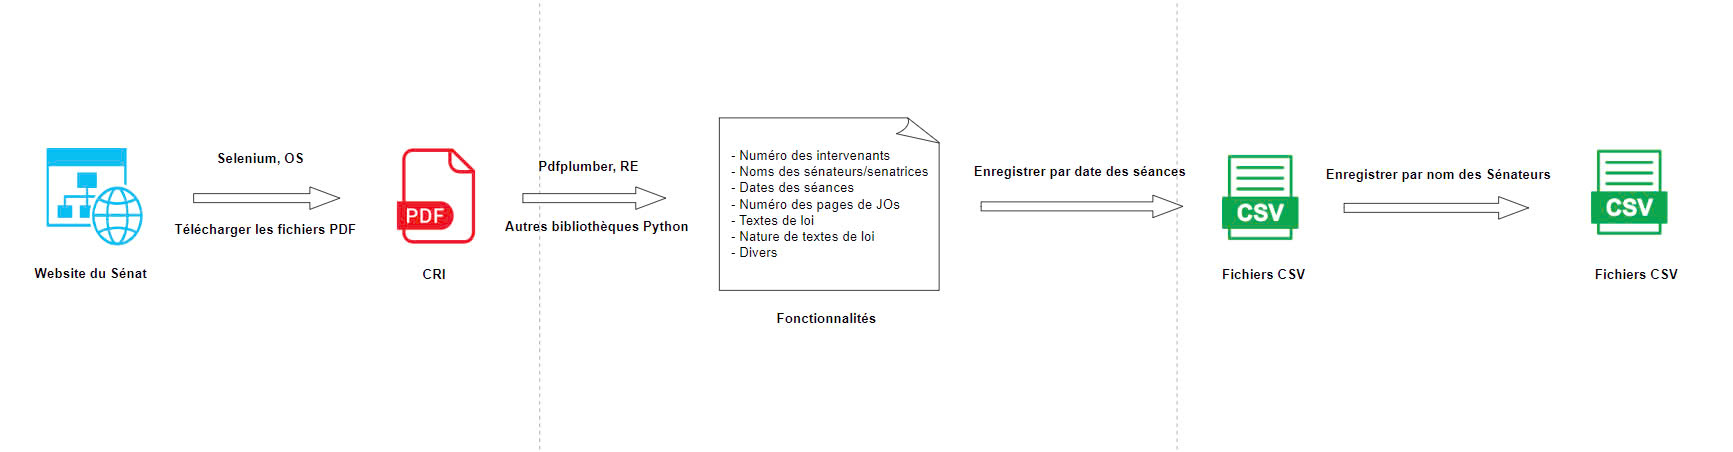
\includegraphics[width=\linewidth]{images/schemas les etapes de travail.jpg} % Đặt đường dẫn đúng tới ảnh của bạn
    \caption{Schéma des étapes de travail}
    \label{fig:schema_travail}
\end{figure}

\subsection{Explication du script}

Ce processus d'automatisation est conçu pour collecter tous les journaux officiels (JO) de l'année 2022 sur le site du Sénat français. Le script utilise l'outil \gls{selenium} pour automatiser la navigation et le téléchargement des fichiers \gls{PDF} à partir du site suivant : \url{https://www.senat.fr/seances/seances.html}. 
Le script identifie les liens vers les fichiers \gls{PDF}, les télécharge à l'aide de la commande \texttt{curl}, et continue le processus jusqu'à ce que tous les fichiers soient récupérés.

\subsubsection{a. Configuration de l'environnement et des bibliothèques}

La première étape consiste à configurer l'environnement et à importer les bibliothèques nécessaires. \gls{selenium} est celle utilisée pour l'automatisation du navigateur, \texttt{os} pour la gestion des fichiers, et \texttt{subprocess} pour exécuter des commandes système telles que \texttt{curl}.

\begin{lstlisting}[language=Python]
from selenium import webdriver
from selenium.webdriver.common.by import By
from selenium.webdriver.common.action_chains import ActionChains
from selenium.webdriver.common.keys import Keys
from selenium.webdriver.support.ui import WebDriverWait
from selenium.webdriver.support import expected_conditions as EC
import time
import os
import subprocess
\end{lstlisting}

\subsubsection{b. Création du dossier pour stocker les fichiers PDF}

Avant de télécharger les fichiers, nous devons créer un dossier pour les stocker. Si ce dossier n'existe pas, il est créé automatiquement.

\begin{lstlisting}[language=Python]
download_dir = "/content/cri_pdf"

if not os.path.exists(download_dir):
    os.makedirs(download_dir)
\end{lstlisting}

\subsubsection{c. Fonction pour télécharger un fichier PDF avec \texttt{curl}}

Cette fonction utilise la commande \texttt{curl} pour télécharger un fichier PDF à partir d'une URL et l'enregistrer dans le dossier spécifié.

\begin{lstlisting}[language=Python]
def download_with_curl(url, download_dir, filename):
    file_path = os.path.join(download_dir, filename)
    subprocess.run(["curl", "-o", file_path, url], check=True)
\end{lstlisting}

\subsubsection{d. Lancement du navigateur et ouverture de la page web}

Ensuite, nous lançons le navigateur Chrome et accédons à la page web du Sénat, où sont répertoriées les séances. Nous attendons que la page se charge avant de procéder.

\begin{lstlisting}[language=Python]
driver = webdriver.Chrome()
driver.get('https://www.senat.fr/seances/seances.html')
time.sleep(5)  # On attend 5 secondes pour que la page se charge
\end{lstlisting}

\subsubsection{e. Utilisation de \texttt{ActionChains} pour faire défiler la page et cliquer sur un bouton}

Pour interagir avec la page, nous utilisons la classe \gls{actionchains} pour simuler des actions comme le défilement et le clic sur des boutons identifiés par leur chemin \gls{xpath} (XML Path Language)

\begin{lstlisting}[language=Python]
actions = ActionChains(driver)

xpath_to_button = '/html/body/main/article/div/div/div/div[1]/div/div[2]/div[1]/div/div/div[3]/h2/button'

while True:
    try:
        WebDriverWait(driver, 10).until(
            EC.element_to_be_clickable((By.XPATH, xpath_to_button))
        ).click()
        time.sleep(3)
\end{lstlisting}

\subsubsection{f. Recherche et traitement des liens vers les fichiers PDF}

Nous identifions une section spécifique de la page contenant des liens vers les fichiers \gls{PDF}. Cette section est identifiée grâce à son chemin \gls{xpath}, et tous les liens sont récupérés.

\begin{lstlisting}[language=Python]
        xpath_to_links_container = '/html/body/main/article/div/div/div/div[1]/div/div[2]/div[1]/div/div/div[3]'
        links_container = WebDriverWait(driver, 10).until(
            EC.presence_of_element_located((By.XPATH, xpath_to_links_container))
        )
        links = links_container.find_elements(By.TAG_NAME, 'a')
\end{lstlisting}

\newpage
\subsubsection{g. Recherche et téléchargement des fichiers PDF}

Le script parcourt ensuite chaque lien trouvé. Pour chaque lien contenant la mention "et au format PDF", l'URL du fichier est récupérée et son contenu téléchargé à l'aide de la fonction \texttt{download\_with\_curl()}.

\begin{lstlisting}[language=Python]
        original_tab = driver.current_window_handle

        for link in links:
            try:
                href = link.get_attribute('href')  # On récupère l'URL du lien
                if href:  # Vérifie si le lien existe
                    driver.get(href)  # Ouvre le lien
                    time.sleep(2)

                    pdf_links = driver.find_elements(By.PARTIAL_LINK_TEXT, "et au format PDF")
                    for pdf_link in pdf_links:
                        try:
                            pdf_href = pdf_link.get_attribute('href')
                            if pdf_href:
                                print(f"URL du fichier PDF: {pdf_href}")

                                file_base = pdf_href.split('/')[-1].split('.')[0]  # Nom du fichier
                                new_filename = f"{file_base}.pdf"  # Nouveau nom du fichier

                                download_with_curl(pdf_href, download_dir, new_filename)

                                time.sleep(5)
\end{lstlisting}

\newpage
\subsubsection{h. Retour à la page précédente et défilement}

Après le téléchargement d'un fichier \gls{PDF}, le script retourne à la page précédente pour traiter les autres liens. En cas d'erreur, il fait défiler la page pour essayer le suivant.

\begin{lstlisting}[language=Python]
                    driver.back()  # Retour à la page précédente
                    time.sleep(2)
            except Exception as e:
                print(f"Impossible de cliquer sur le lien: {e}")

        break
    except Exception as e:
        actions.send_keys(Keys.PAGE_DOWN).perform()
        time.sleep(1)
\end{lstlisting}

\subsubsection{i. Fermeture du navigateur}

Une fois tous les liens traités, le navigateur se ferme pour libérer de la mémoire.

\begin{lstlisting}[language=Python]
driver.quit()
\end{lstlisting}

\section{Étapes d'automatisation de l'extraction}

\subsection{Importation des bibliothèques}

Les lignes de commande ci-dessous importent les bibliothèques nécessaires à la bonne exécution du script : \texttt{os} permet de travailler avec les fichiers et dossiers, \texttt{pdfplumber} est utilisé pour lire et extraire des informations des fichiers PDF, \texttt{pandas} est utilisé pour manipuler les données sous forme de tableaux (DataFrame), et \texttt{shutil} pour copier des fichiers d'un dossier à un autre.

\begin{lstlisting}
import os
import pdfplumber
import pandas as pd
import shutil
\end{lstlisting}
\subsection{2. Fonction \texttt{extract\_bold\_lines\_from\_all\_pages}}
Cette fonction permet d'extraire les lignes de texte en gras de chaque page d'un fichier PDF, \texttt{pdfplumber} est utilisé pour parcourir chaque page et récupérer les mots et groupes de caractères en gras (ce qui est vérifié grâce à la balise \texttt{"Bold"} dans le nom de la police). Si l'un d'eux ne fait pas partie de la liste des termes déjà enregistrés, il est ajouté à cette dernière, puis la boucle continue. 
Dès qu'une ligne complète en gras est détectée, elle est ajoutée à une liste avec le numéro de page correspondant. La fonction renvoie ensuite la liste complète des lignes en gras avec leurs numéros de page individuel.
\begin{lstlisting}
def extract_bold_lines_from_all_pages(pdf_path):
    bold_lines = []
    with pdfplumber.open(pdf_path) as pdf:
        for page_number in range(len(pdf.pages)):
            current_line = ""
            page = pdf.pages[page_number]
            chars = page.chars
            for char in chars:
                if "Bold" in char["fontname"]:
                    current_line += char["text"]
                elif current_line.strip():
                    bold_lines.append((page_number + 1, current_line.strip()))  
                    current_line = ""
            if current_line.strip():
                bold_lines.append((page_number + 1, current_line.strip()))  
    return bold_lines
\end{lstlisting}
\newpage
\subsection{Fonction \texttt{extract\_honorifics}}
Cette fonction extrait les noms des intervenants en fonction de certains préfixes spécifiques (comme \texttt{"Mme le"}, \texttt{"M. le"}, etc.). Elle parcourt les lignes en gras extraites précédemment et recherche ces préfixes. 
Lorsqu'un nom d'intervenant est trouvé, il est enregistré avec le numéro de page correspondant. La fonction retourne ensuite une liste des noms d'intervenants et des numéros de pages.
\begin{lstlisting}
def extract_honorifics(bold_lines):
    honorific_prefixes = ['Mme le', 'Mme la', 'M. le', 'M.', 'Mme']
    extracted_honorifics = []
    page_values = {}
    for page_number, text in bold_lines:
        if text.isdigit():
            page_values[page_number] = text
    for page_number, text in bold_lines:
        for prefix in honorific_prefixes:
            if prefix in text:
                start_index = text.find(prefix)
                end_index = start_index + len(prefix) 
                for i in range(end_index, len(text)):
                    if text[i] in ['.', ',']:
                        end_index = i + 1
                        break
                page_value = page_values.get(page_number, "")
                extracted_honorifics.append((text[start_index:end_index].strip(), page_value))
                break
    return extracted_honorifics
\end{lstlisting}

\newpage
\subsection{Fonction \texttt{process\_pdf\_file}}
Cette section traite chaque fichier \gls{PDF} dans le répertoire spécifié, en extrait les informations avec les fonctions ci-dessus, puis exporte les résultats dans des fichiers \gls{csv} qui sont enregistrés dans un dossier de sortie. La date est extraite du nom du fichier \gls{PDF}, puis formatée afin d'être ajoutée dans le tableau des résultats.
\begin{lstlisting}

def process_pdf_file(pdf_path, date):
    bold_lines = extract_bold_lines_from_all_pages(pdf_path)
    honorifics = extract_honorifics(bold_lines)
    df = pd.DataFrame(honorifics, columns=['Nom_intervenants', 'Num_page'])
    if not df.empty:
        first_president_row = df[(df['Nom_intervenants'] == 'Mme la présidente.') |
                                 (df['Nom_intervenants'] == 'Mme le présidente.') |
                                 (df['Nom_intervenants'] == 'M. le président.') |
                                 (df['Nom_intervenants'] == 'Mme le président.') |
                                 (df['Nom_intervenants'] == 'Mme la président.')].index[0]
        df = df[first_president_row:]
        df['Numero'] = range(1, len(df) + 1)
        df['Date_seances'] = date
        df = df[['Numero', 'Nom_intervenants', 'Date_seances', 'Num_page']]
    return df
\end{verbatim}

Cette fonction prend en entrée un fichier PDF et une date. Elle utilise les fonctions précédentes pour extraire les lignes en gras et les noms des intervenants. Ensuite, elle filtre les noms des intervenants à partir du premier président identifié dans la séance. 
Le résultat est sauvegardé sous forme de tableau avec un numéro d'ordre, le nom de l'intervenant, la date de la séance et le numéro de page.

\subsection{5. Boucle de traitement des fichiers PDF}
\begin{verbatim}
data_dir = "/content/cri_pdf"
output_dir = "/content/compte_intervenants_et_pages"
os.makedirs(output_dir, exist_ok=True)
pdf_files = [f for f in os.listdir(data_dir) if f.endswith('.pdf')]
french_months = ["janvier", "février", "mars", "avril", "mai", "juin", "juillet", "août", "septembre", "octobre", "novembre", "décembre"]
for pdf_file in pdf_files:
    pdf_path = os.path.join(data_dir, pdf_file)
    filename = os.path.splitext(pdf_file)[0]
    year, month, day = filename[1:5], filename[5:7], filename[7:9]
    month_name = french_months[int(month) - 1]
    date = f"{day} {month_name} {year}"
    df = process_pdf_file(pdf_path, date)
    if not df.empty:
        csv_file_name = f"{filename}.csv"
        csv_file_path = os.path.join(output_dir, csv_file_name)
        df.to_csv(csv_file_path, index=False, encoding='utf-8-sig')
\end{lstlisting}
\subsection{Filtrage des noms et copie des fichiers}
Cette partie filtre les fichiers \gls{csv} basés sur une liste de noms d'intervenants prédéfinis et copie les fichiers correspondants dans un autre répertoire. Elle utilise \texttt{shutil.copy2} pour copier chaque fichier tout en préservant ses métadonnées.
\begin{lstlisting}
import shutil
source_folder = 'D:/document/stage/Output'
destination_folder = 'D:/document/stage/Output/filter'
os.makedirs(destination_folder, exist_ok=True)
formatted_names = [...]  # Liste des noms formatés
for filename in os.listdir(source_folder):
    if filename.endswith('.csv'):
        file_name_without_extension = os.path.splitext(filename)[0]
        if file_name_without_extension in formatted_names:
            source_file_path = os.path.join(source_folder, filename)
            destination_file_path = os.path.join(destination_folder, filename)
            shutil.copy2(source_file_path, destination_file_path)
            print(f"File copied: {filename}")
\end{lstlisting}
\subsection{Extraction de sujet et des textes de loi}

\subsubsection{Suppression des termes indésirables}

La première étape consiste à définir une fonction appelée \texttt{remove\_unwanted\_terms()} qui permet de supprimer certains termes indésirables qui apparaissent fréquemment dans le fichier \gls{PDF} mais qui ne sont pas pertinents pour l'extraction des titres. Ces termes incluent des phrases comme "Mme la présidente" ou "M. le président", qui sont souvent répétitifs mais ne fournissent pas d'information utile pour atteindre notre objectif. 

Cette fonction parcourt chaque ligne de texte et remplace les termes indésirables par une chaîne vide, puis renvoie la ligne de texte ainsi nettoyée.

\begin{lstlisting}[language=Python]
def remove_unwanted_terms(text):
    unwanted_terms = [
        'Mme la présidente.',
        'Mme le présidente.',
        'M. le président.',
        'Mme le président.',
        'Mme la président.'
    ]
    for term in unwanted_terms:
        text = text.replace(term, '')
    return text.strip()
\end{lstlisting}
Dans cet exemple, chaque terme indésirable contenu dans le texte est remplacé par une chaîne vide. La fonction \texttt{strip()} est utilisée pour supprimer les espaces en trop après le nettoyage. Cela garantit que les phrases indésirables ne soient plus présentes dans le résultat final.

\subsection{Extraction des titres et du texte}

La fonction principale \texttt{extract\_Titre\_Texte()} est utilisée pour analyser le contenu du fichier \gls{PDF}, page par page, et extraire les sections pertinentes. Elle se concentre principalement sur l'extraction des parties du texte qui sont en gras (ce qui correspond généralement aux titres) ainsi que des sections contenant certains mots-clés, tels que "Article", "Après l’article", ou "Avant l’article", qui sont les indicateurs de sections importantes du document.

\subsubsection{Ouverture du fichier PDF et lecture des caractères}

La fonction commence par ouvrir le fichier \gls{PDF} avec la bibliothèque \texttt{pdfplumber}. Ensuite, elle parcourt chaque page du document et analyse les caractères présents sur chaque ligne pour détecter ceux qui sont en gras. Les caractères en gras sont généralement associés aux titres, c'est pourquoi cette détection est essentielle pour la structuration des données.
\begin{lstlisting}
def extract_Titre_Texte(pdf_path):
    data = []
    expected_number = 1  # Variable pour suivre le numéro attendu
    with pdfplumber.open(pdf_path) as pdf:
        for page_number in range(len(pdf.pages)):
            current_line = ""
            page = pdf.pages[page_number]
            chars = page.chars  # 'chars' est un dictionnaire des caractères

            for char in chars:
                if "Bold" in char["fontname"]:  # Si le caractère est en gras
                    current_line += char["text"]  # Ajoute le texte en gras
                elif current_line.strip():  # Si la ligne est terminée
                    match = re.match(r"(\d+)\s+([A-Za-zÀ-Ýa-zà-ý\s:’.,;?!()\[\]«»\-]*)(?:\s*(Mme la présidente\.|Mme le présidente\.|M\. le président\.|Mme le président\.|Mme la président\.))?$", current_line.strip())
                    if match and int(match.group(1)) == expected_number:
                        expected_number += 1  # Incrémenter le numéro attendu
                        title_text = f"{match.group(2).strip()}"
                        data.append((page_number + 1, current_line.strip(), title_text, ""))
                    else:
                        data.append((page_number + 1, current_line.strip(), None, ""))
                    current_line = ""
\end{lstlisting}
Dans cet extrait de code, la fonction vérifie chaque caractère pour déterminer s'il est en gras (reconnaissable grâce à l'attribut \texttt{"Bold"} dans le nom de la police). Lorsque des caractères en gras sont détectés, ils sont concaténés dans une chaîne de texte qui est ensuite traitée comme un titre potentiel.

\subsubsection{Traitement des fins de pages et suppression des termes indésirables}

À la fin de chaque page, il est possible que certaines informations non pertinentes, comme des numéros de page, apparaissent. La fonction \texttt{remove\_unwanted\_terms()} est ensuite appelée pour supprimer ces éléments indésirables dans les titres avant de finaliser les données extraites.

\begin{lstlisting}[language=Python]
# Supprimer les mots non souhaités à la fin du texte (Mme la présidente) du TITRE
for i in range(len(data)):
    if data[i][2] is not None:
        data[i] = (data[i][0], data[i][1], remove_unwanted_terms(data[i][2]), data[i][3])
\end{lstlisting}
Cette boucle parcourt les données extraites, vérifie si le titre contient l'un des termes indésirables, et applique la fonction \texttt{remove\_unwanted\_terms()} pour nettoyer les résultats.

\subsubsection{Remplissage des valeurs manquantes et détection du texte}

Une fois les titres extraits et nettoyés, les valeurs manquantes sont comblées. Si une ligne n'a pas de titre explicite, le titre de la ligne précédente est utilisé. De même, les sections contenant les mots-clés comme "Article", "Après l’article", ou "Avant l’article" sont identifiées et ajoutées à la colonne \textbf{Texte}.
\begin{lstlisting}
# Remplacer les valeurs 'none' ou vides par celles du Titre précédent
last_titre_text = None
for i in range(len(data)):
    if data[i][2] is not None:
        last_titre_text = data[i][2]
    elif last_titre_text is not None:
        data[i] = (data[i][0], data[i][1], last_titre_text, data[i][3])

# Si les valeurs en gras contiennent des termes tels que : Après l’article, Article, Avant l’article, les ajouter à la liste (thème)
for i in range(len(data)):
    if data[i][1] and ("Après l’article" in data[i][1] or "Article" in data[i][1] or "Avant l’article" in data[i][1]):
        data[i] = (data[i][0], data[i][1], data[i][2], data[i][1])
\end{lstlisting}

Dans ce processus, la fonction remplit les valeurs manquantes en utilisant les titres précédents pour garantir qu'aucune ligne ne soit laissée vide. Ensuite, elle identifie les sections textuelles pertinentes à l'aide de mots-clés spécifiques.

\subsubsection{Fonction \texttt{extract\_topic} pour extraire la nature des articles de loi}

La fonction \texttt{extract\_topic()} est utilisée pour extraire les informations relatives aux thèmes à partir d’un fichier \gls{PDF}. Ces thèmes pertinents incluent des zones de texte en majuscules mais non en gras, et qui contiennes, par exemple, les termes "PROPOSITION DE LOI" ou "PROJET DE LOI". La variable \texttt{topic\_lines} est quant à elle appelée comme liste vide dont le rôle et de lister ces lignes de texte correspondantes aux thèmes identifiés.

\begin{lstlisting}[language=Python]
def extract_topic(pdf_path, data):
    topic_lines = []
\end{lstlisting}

Ensuite, la fonction utilise \texttt{\gls{pdfplumber}} pour ouvrir et lire le contenu du fichier \gls{PDF}. Ce dernier est ouvert à l'aide de \texttt{pdfplumber.open()}, et chaque page du fichier est parcourue via une boucle \texttt{for}. Les caractères sur chaque page sont extraits.

\begin{lstlisting}[language=Python]
with pdfplumber.open(pdf_path) as pdf:
    for page_number in range(len(pdf.pages)):
        current_line = ""
        page = pdf.pages[page_number]
        chars = page.chars
\end{lstlisting}

Le code vérifie chaque caractère pour déterminer s'il est en gras ou non (en se basant sur l'attribut \texttt{Bold} dans \texttt{fontname}). Si le caractère n'est pas en gras, il est ajouté à la chaîne \texttt{current\_line}.

\begin{lstlisting}[language=Python]
for char in chars:
    if "Bold" not in char["fontname"]:
        current_line += char["text"]
\end{lstlisting}

Une fois que les caractères non en gras sont collectés, le code vérifie si la chaîne \texttt{current\_line} contient l'une des expressions "PROPOSITION DE LOI" ou "PROJET DE LOI". Si l'une des expressions est trouvée, la ligne de texte actuelle, ainsi que le numéro de page, sont ajoutés à la liste \texttt{topic\_lines}.

\begin{lstlisting}[language=Python]
if "PROPOSITION DE LOI" in current_line or "PROJET DE LOI" in current_line:
    topic_lines.append((page_number + 1, current_line))
\end{lstlisting}

\newpage
Après avoir collecté les lignes de texte relatives au thème, le code utilise des expressions régulières (\gls{regex}) pour rechercher et extraire avec précision les parties du texte contenant "PROPOSITION DE LOI" ou "PROJET DE LOI".

\begin{lstlisting}[language=Python]
pattern_proposition = r'\b[A-ZÀ-Ý\s\.,;’!?()_-]*PROPOSITION DE LOI[A-ZÀ-Ý\s\.,;’!?()_-]*\b'
matches_proposition = re.findall(pattern_proposition, text, re.DOTALL)

pattern_projet = r'\b[A-ZÀ-Ý\s\.,;’!?()_-]*PROJET DE LOI[A-ZÀ-Ý\s\.,;’!?()_-]*\b'
matches_projet = re.findall(pattern_projet, text, re.DOTALL)
\end{lstlisting}
Les modèles d'expressions régulières \texttt{pattern\_proposition} et \texttt{pattern\_projet} recherchent les expressions "PROPOSITION DE LOI" et "PROJET DE LOI" dans le texte, avec des caractères en majuscules, espaces, ponctuations avant et après. 

Les résultats extraits par les \gls{regex} sont ensuite nettoyés. Les espaces multiples sont remplacés par un seul, et les caractères spéciaux au début et à la fin de la chaîne sont supprimés. Le processus fonctionne de la sorte : tout d'abord, les espaces multiples dans la chaîne \texttt{match} sont remplacés par un seul espace via la fonction \texttt{re.sub}. Ensuite, les caractères indésirables au début et à la fin de la chaîne sont retirés automatiquement par la fonction.
\begin{lstlisting}[language=Python]
cleaned_match = re.sub(r'\s+', ' ', match.strip())
cleaned_match = re.sub(r'^[\s\.,;’!?()_-]+|[\s\.,;’!?()_-]+$', '', cleaned_match)
\end{lstlisting}
Le code vérifie ensuite si le dernier mot de la chaîne est trop court (moins de 2 caractères), si c’est le cas, il est supprimé. Cela permet de s'assurer que les mots incomplets ou trop courts ne sont pas conservés dans le résultat final.
\begin{lstlisting}[language=Python]
while words and len(words[-1]) < 2:
    words.pop()
cleaned_match = ' '.join(words)
\end{lstlisting}
Enfin, le thème est ajouté aux données d'origine (\texttt{data}) en fonction du numéro de page. Si une page a un thème, il est ajouté à la cinquième colonne de chaque ligne.
\begin{lstlisting}[language=Python]
for i in range(len(data)):
    page_number = data[i][0]   
    if page_number in theme_lines:
        data[i] = (data[i][0], data[i][1], data[i][2], data[i][3], theme_lines[page_number])
\end{lstlisting}
Si une ligne ne contient pas de thème, le code remplace cette valeur par le thème de la page précédente. Cela garantit que toutes les lignes ont un thème, sans laisser de colonne vide.
\begin{lstlisting}
last_topic_text = ""
for i in range(len(data)):
    if len(data[i]) > 4 and data[i][4] != "":
        last_topic_text = data[i][4]
    else:
        data[i] = (data[i][0], data[i][1], data[i][2], data[i][3], last_topic_text)
\end{lstlisting}
Enfin, les données traitées, avec les thèmes associés à chaque page du fichier \gls{PDF}, sont retournées par la fonction.
\begin{lstlisting}[language=Python]
return data
\end{lstlisting}
Ce processus permet d’identifier et d’extraire efficacement les informations liées à des propositions ou projets de loi à partir de fichiers \gls{PDF} complexes, en les organisant de manière structurée pour une utilisation ultérieure.


\section{Évaluation des performances}

\subsection{Qualité de l’éxtraction}


\begin{table}[ht!]
\centering
\begin{tabular}{|c|p{8cm}|}
\hline
\textbf{Nom de colonne} & \textbf{Description} \\
\hline
Numero & Numéro d'intervenant \\
\hline
Date\_seances & Date des séances publiques \\
\hline
Num\_page & Numéro des pages du \textit{Journal Officiel} \\
\hline
Titre & Divers, sujet général de contenu de discussion \\
\hline
Texte & L'article de loi discuté \\
\hline
Thème & Nature du texte des articles de loi \\
\hline
\end{tabular}
\caption{Description des colonnes du fichier CSV}
\label{table:description_csv}
\end{table}


\subsubsection{Partie 1: Numérotation des intervenants, Nom des Sénateurs, Numéro de pages}

Après plusieurs ajustements du script d'extraction automatique, notamment l'optimisation des algorithmes de reconnaissance de motifs et l'amélioration de la gestion des lignes en gras pour identifier les intervenants, les résultats obtenus ont montré une précision considérablement améliorée. De plus, lorsque l'extraction automatisée est comparée à l'entrée manuelle, la méthode automatisée produit de meilleurs résultats et se montre plus rapide rapide, avec une réduction significative des erreurs.

Les chaînes d'extraction ajustées ont fonctionné de manière efficace en isolant correctement les noms des intervenants, les numéros de page, et d'autres métadonnées critiques des documents \gls{PDF}. En particulier, les améliorations apportées au traitement des textes en gras ont permis de capturer les noms et les numéros d'intervenants avec une précision bien supérieure. En effet, dans les étapes précédentes, certaines erreurs pouvaient apparaître, notamment lorsque plusieurs intervenants étaient affichés sur la même page, ou dans le cas où des titres non pertinents étaient pris en compte. Grâce aux ajustements, ces erreurs ont été corrigées, permettant une identification plus claire et précise des informations pertinentes.
Le résultat est un total de 85 fichier \gls{CSV} correspondant aux 85 sessions de l'année 2022, pour comparer facilement la précision de l'extraction, voici 2 captures d'écran des résultats de test de l'application \gls{Prepub} ainsi que le tableau issu du processus d'automatisation au 22 février 2022 :

\begin{figure}[H]
    \centering
    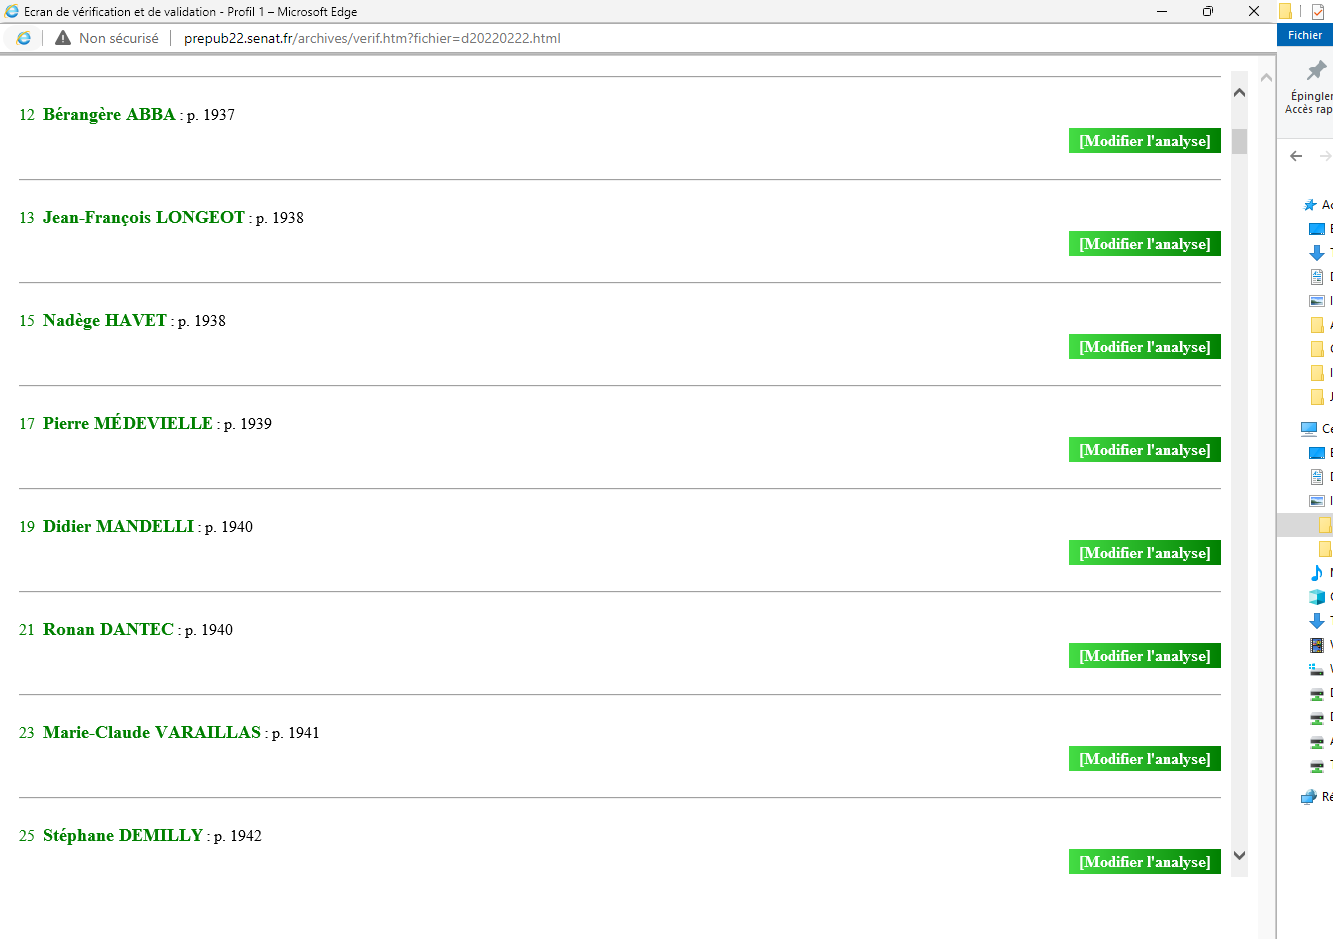
\includegraphics[width=1\textwidth]{images/check 4.PNG}
    \caption{Capture d'écran de vérification et de validation d'application archives Prépub}
\end{figure}

\begin{figure}[H]
    \centering
    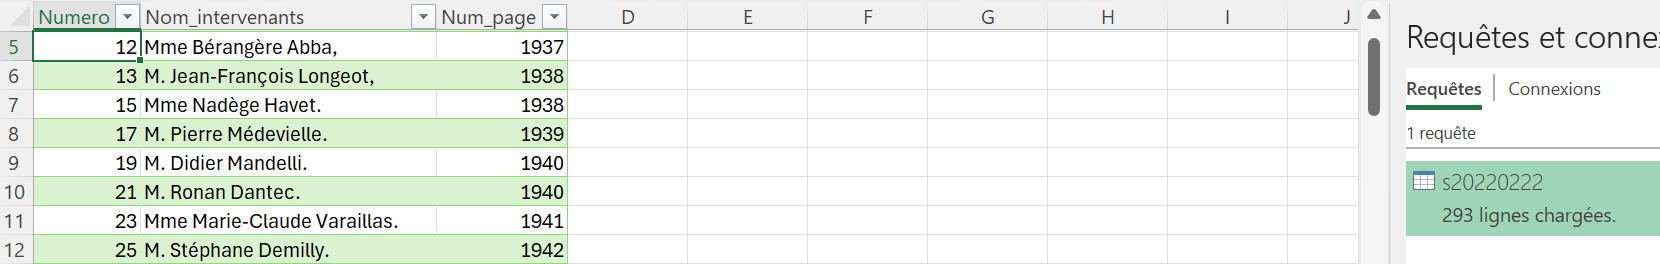
\includegraphics[width=1\textwidth]{images/verifie4.png}
    \caption{Capture d'écran de tableaux extrait}
\end{figure}

Nous pouvons voir que les numéros des intervenants se correspondent parfaitement sur les deux résultats : 12, 13, 15, 17, 19, 21, 23, 25... .\\
Concernant le nom des intervenants, ils sont également identiques, cependant, sur les photos du site, ces derniers sont écrits en majuscules pour les noms de famille (par exemple Bérangère ABBA au lieu de Mme Bérangère Abba) ; de même, les titres « Mme » et « M ». n'apparaissent pas dans la capture d'écran du site Web, car seuls le prénom et nom de famille sont affichés. Nous pouvons cependant, grâce à un script, exécuter une commande afin de nettoyer cette mise en forme et mettre tous les noms de famille des orateurs en majuscule. .\\
Enfin, les numéros de page se correspondent également parfaitement : 1937, 1938, 1939, 1940, 1941, 1942. De plus, la date de la session est extraite du nom du fichier de la session au format saaaammdd (s = séance; aaaa = année; mm= mois, dd=date), les résultats seront donc précis et correspondront aux autres informations extraites de la session du jour.

\newpage
\subsubsection{Partie 2: Textes de loi, Nature de textes, Divers}

Prenons l'exemple de la table des matières de la Sénatrice Mélanie Vogel.

\begin{figure}[H]
    \centering
    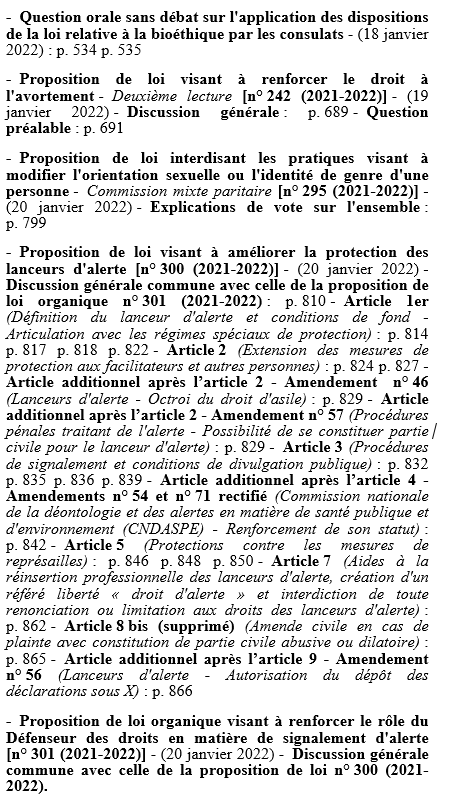
\includegraphics[width=0.7\textwidth]{images/check5table.png}
    \caption{Capture d'écran de table du Sénat de Mme Mélanie Vogel 2022}
\end{figure}

\begin{figure}[H]
    \centering
    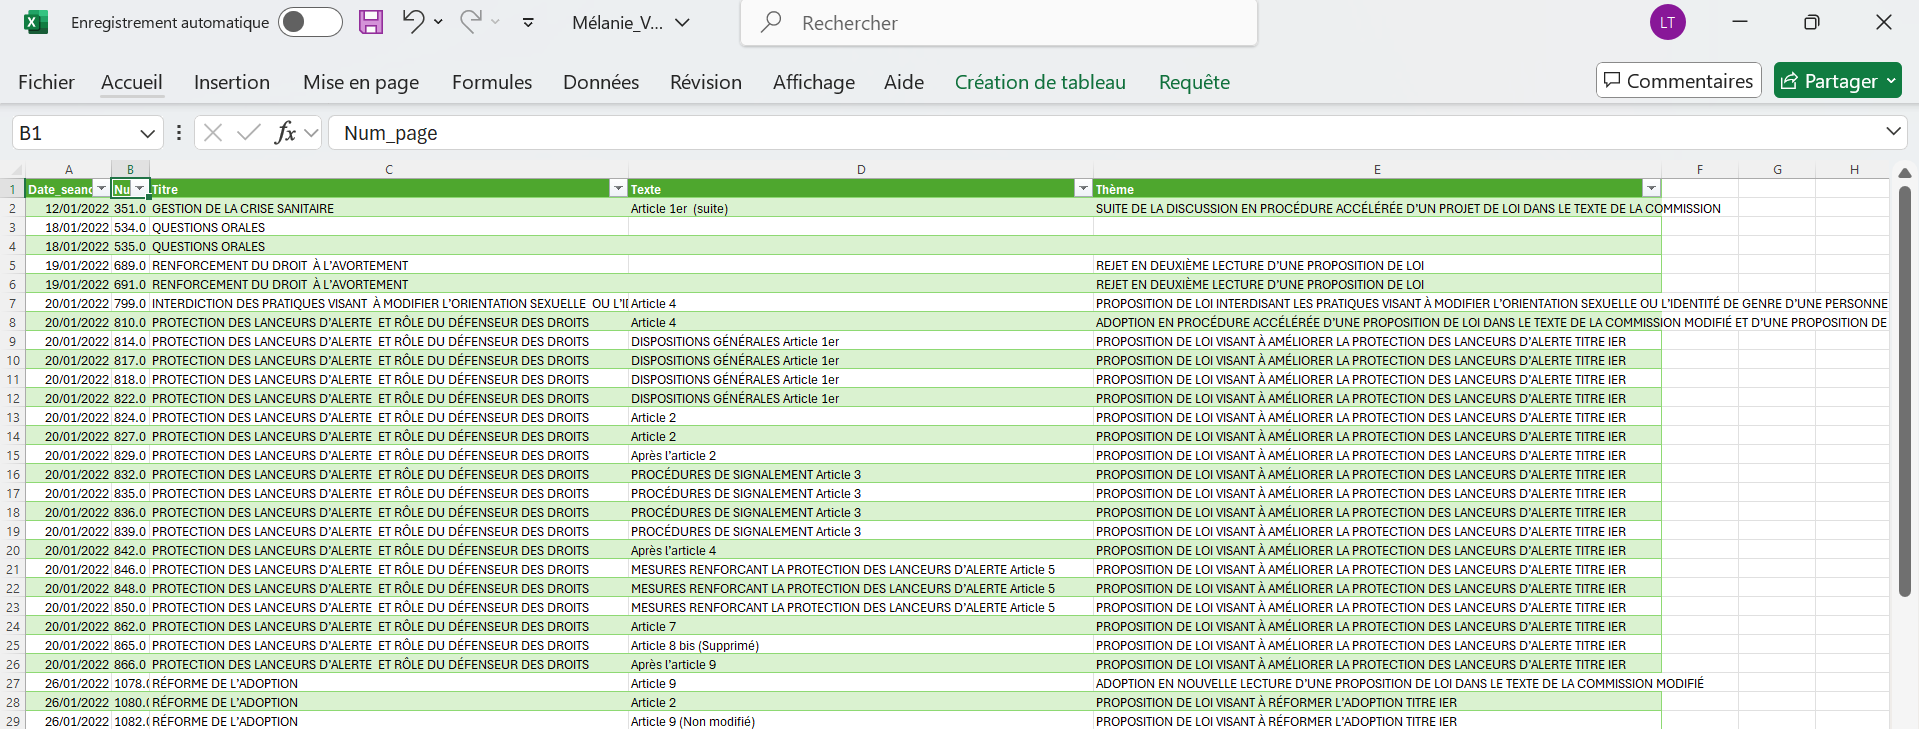
\includegraphics[angle=90, width=0.6\textwidth]{images/Capture d'écran 2024-09-28 034312.png}
    \caption{Capture d'écran de tableaux extrait automatique}
\end{figure}

\paragraph{} On note la présence de beaucoup d'informations détaillées dans les tables du Sénat, à la fois complètes et précise, incluant des éléments comme : les sujets, les dates, les numéros de page, les types de documents, et des contenus supplémentaires comme les questions, les discussions générales, etc. En ce qui concerne le tableau extrait automatiquement, il manque des informations sur les thèmes, et la colonne du texte retire parfois des informations non pertinentes. Cela complique la recherche d'informations dans le tableau lorsqu'il est nécessaire de les comparer avec les documents originaux. Bien que l'extraction automatique ait permis de récupérer une partie des titres et des articles avec précision, les informations complémentaires importantes ne sont pas encore suffisantes pour en faire une table des matières complète.

En termes de précision de la structure et de mise en forme dans la table des matières du Sénat, les éléments sont bien formatés, avec des espaces et des signes clairement définis. Cependant, dans le tableau automatisé, bien que le contenu principal soit extrait, la mise en forme n'est pas toujours normalisée. Par exemple, certaines parties extraites sont répétées plusieurs fois, avec des espaces ou des ponctuations inutiles, ce qui entraîne une confusion au niveau de l’apparence. Les symboles spéciaux, comme les guillemets ou les informations sur l'état de modification (par exemple "Article 8 bis (supprimé)"), ne sont pas traités de manière cohérente. En outre, en termes d'exhaustivité du contenu, certains articles peuvent ne pas être complètement extraits ou il peut en manquer certaines parties, en particulier lorsque les titres sont trop longs ou possèdent une structure complexe. Cette situation crée un écart dans l'exhaustivité des informations par rapport à la table des matières réelle. Dans cette dernière, des informations telles que "Proposition de loi n° 300", "Adoption en nouvelle lecture", "Débat sur..." sont entièrement et précisément notées. Pour expliquer cette extraction partielle du contenu, nous pouvons prendre l'exemple de la ligne "Question orale sans débat sur l'application des dispositions de la loi relative à la bioéthique par les consulats" qui, dans le tableau automatisé, n'a extrait que "QUESTIONS ORALES". La partie "sur l'application des dispositions de la loi relative à la bioéthique par les consulats" n'apparaît pas dans le PDF du JO, car cette partie est ajoutée manuellement, et n'est donc pas disponible pour l'extraction automatique.

Nous constatons d'ailleurs que les tables des matières du Sénat ne répètent généralement pas plusieurs fois les mêmes articles ou les informations redondantes. Cependant, dans le tableau automatisé, l'extraction automatique est encore trop brute et peut parfois conduire à des informations répétées, avec des contenus superposés, par exemple, "Proposition de loi visant à améliorer la protection des lanceurs d'alerte" qui apparaît à plusieurs reprises.


\subsection{Limites}

En ce qui concerne la numérotation des intervenants, les scripts sont configurés pour compter les éléments en gras au début des lignes, comme "M." et "Mme" suivis du nom propre et d'un point "." ou d'une virgule ",". Cependant, dans certains cas exceptionnels, comme illustré ci-dessous, le début de ligne en gras ne commence pas par "M." ou "Mme", mais par la phrase \textit{"Plusieurs sénateurs du groupe Les Républicains. Il n’a pas répondu !"}. Cela signifie que ces cas particuliers ne sont pas pris en compte dans le comptage automatique. Bien que cela n'affecte ni le numéro de page ni le contenu de la table des matières, cela peut créer un décalage dans le décompte des intervenants par rapport à la numérotation affichée dans \gls{Prepub}. 

Dans ces cas rares, il est possible de modifier le script pour corriger ce problème de manière spécifique. Cependant, il est important de noter qu'aucun outil d'automatisation ne peut garantir une précision absolue, et que, par conséquent, des vérifications manuelles et des corrections ponctuelles sont parfois inévitables.

\begin{figure}[H]
    \centering
    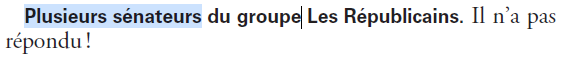
\includegraphics[width=0.7\textwidth]{images/Capture d'écran 2024-09-28 041223.png}
    \caption{Capture d'écran d'un JO}
\end{figure}

En outre, en ce qui concerne l'extraction des thèmes, l'automatisation présente encore plusieurs aspects à améliorer. L'ajout d'informations telles que les numéros de page, les dates et d'autres détails supplémentaires est essentiel pour que l'automatisation puisse atteindre une qualité équivalente à celle des tables des matières du Sénat. Il faudra également prévoir des étapes supplémentaires de traitement pour éliminer les doublons et les données superflues, afin de garantir que les données extraites soient nettes et précises. Pour les parties contenant de nombreux symboles ou des informations supplémentaires, il sera également indispensable d'améliorer la capacité de reconnaissance et de traitement de ces sections afin d'obtenir des résultats d'extraction encore plus précis.
\newpage
\section{Facilitation de la saisie d’information}

Même s'il est actuellement impossible d'automatiser complètement la création des Tables du Sénat, nous pouvons tout de même tirer parti de certaines colonnes du fichier \gls{csv}, notamment le numéro d'intervention, le nom de l'intervenant, et le numéro de page. Ces informations peuvent être intégrées avec un haut niveau de précision dans un fichier \gls{XML}, fichier qui pourra ensuite être chargé dans l'application \gls{Prepub} pour valider les comptes rendus des séances ou pourra servir à générer des tables des matières dans des formats tels que Word à travers la Direction d'Information du Sénat.
Le processus de conversion des données d'un fichier \gls{csv}vers un format \gls{XML} repose sur plusieurs étapes importantes. Tout d'abord, l'utilisation de la bibliothèque `\gls{pandas}` qui permet de lire le fichier CSV et d'organiser ses données sous forme de DataFrame. Le tableau ainsi généré contient des colonnes telles que "Num\_page", "Numero" et "Nom\_intervenants", représentant respectivement le numéro de page, le numéro d'intervention et le nom de l'intervenant. Une fois ces données organisées, la transformation en \gls{XML} nécessite la création de balises spécifiques. Par exemple, une balise `<cri:intervenant>` est utilisée pour encapsuler les informations liées à chaque intervenant. À l'intérieur de cette balise, on insère des attributs comme `nom` pour le nom de l'intervenant, `id` pour le numéro d'intervention et `analyse` pour le numéro de page associé. \footcite{askpython_csv_to_xml}

Ensuite, chaque ligne du DataFrame est parcourue, et pour chaque enregistrement, une nouvelle balise \gls{XML} est générée avec les informations correspondantes. Ces balises sont ensuite organisées dans une structure \gls{XML} hiérarchique où les éléments sont imbriqués selon leur relation avec les autres données. La conversion est réalisée grâce à la méthode `\gls{elementtree}` de la bibliothèque `xml.etree.ElementTree`, qui permet d'écrire les balises générées dans un fichier \gls{XML}.

Ce processus offre de nombreux avantages, notamment la possibilité d'utiliser ces données dans des systèmes qui nécessitent un format standardisé tel que \gls{XML} Cela permet également une interopérabilité accrue avec d'autres outils ou systèmes d'archivage. Une fois les données converties, elles peuvent être intégrées dans des bases de données ou utilisées pour des analyses ultérieures, tout en garantissant un format cohérent et lisible par les machines.


\begin{table}[ht]
    \centering
    \begin{adjustbox}{max width=\textwidth}
    \begin{tabular}{|l|l|p{8cm}|} % Adjust the width of the third column
        \hline
        \textbf{Type d'annotations} & \textbf{Balise XML/Attribut résultant} & \textbf{Copier à la main le XML correspondant} \\ \hline
        \textbf{Nom d’intervenants} & \verb|<cri:intervenant>| \verb|nom=| & \lstinline|<cri:intervenant id="int_11" parid="par_40" mat="12028B" nom="Marie-Arlette CARLOTTI" civ="Mme" qua="" type="1" analyse="p. 4170" checked="O">| \\ \hline
        \textbf{Numéro d'intervention} & \verb|<cri:intervenant>| \verb|id=| & \lstinline|<cri:intervenant id="int_11" parid="par_40" mat="12028B" nom="Marie-Arlette CARLOTTI" civ="Mme" qua="" type="1" analyse="p. 4170" checked="O">| \\ \hline
        \textbf{Numéro de page} & \verb|<cri:intervenant>| \verb|analyse=| & \lstinline|<cri:intervenant id="int_11" parid="par_40" mat="12028B" nom="Marie-Arlette CARLOTTI" civ="Mme" qua="" type="1" analyse="p. 4170" checked="O">| \\ \hline
        \textbf{Article} & \verb|<cri:mentionarticle>| \verb|num=| \verb|info=| & \lstinline|<cri:mentionarticle parid="par_2018" id="debut_detail_loi_22" type="1" num="Article�13" info="Soumission des terminaux méthaniers flottants à un régime administratif propre"><a name="R13"> </a><p class="mention_article" id="par_2018">Article&#160;13</p></cri:mentionarticle>| \\ \hline
    \end{tabular}
    \end{adjustbox}
    \caption{Table des annotations et balises XML correspondantes}
\end{table}






	
	\chapter*{Conclusion}
\markboth{Conclusion}{}
\addcontentsline{toc}{chapter}{Conclusion}
\label{sec:conclusion}
En conclusion, ce mémoire a permis d’explorer les enjeux liés à l’automatisation de la création des tables des matières pour les débats parlementaires au Sénat, à travers l’étude des Journaux Officiels de l’année 2022. Le travail effectué durant le stage s’est concentré sur la compréhension des processus traditionnels, les échanges avec les archivistes, ainsi que sur le développement et la mise en œuvre d’un processus d’automatisation basé sur l’intelligence artificielle.

Les résultats obtenus montrent que l’automatisation peut réduire considérablement le temps et les ressources humaines nécessaires pour gérer les métadonnées des débats, tout en améliorant la précision et la cohérence des informations. Grâce à l’utilisation de bibliothèques Python et d’outils de traitement du langage naturel, ce projet ouvre des perspectives intéressantes pour une future extension de l’automatisation à d’autres corpus de données parlementaires.

Bien que certaines limites demeurent, notamment en ce qui concerne la reconnaissance de certaines entités spécifiques et les défis posés par la qualité variable des données sources, les avancées réalisées permettent d’envisager une mise à l’échelle plus large du processus. Des améliorations techniques, telles que l’intégration de modèles d’apprentissage plus avancés et une meilleure gestion des exceptions, pourraient encore renforcer l’efficacité du processus.

Ainsi, ce mémoire propose une première étape dans la modernisation des méthodes archivistiques du Sénat, et démontre que l’automatisation constitue une voie prometteuse pour répondre aux exigences croissantes de traitement des informations parlementaires tout en garantissant la transparence et l’accessibilité des débats.
	\newpage{\pagestyle{empty}\cleardoublepage}

 %les annexes
	\chapter*{Annexes}
        \addcontentsline{toc}{chapter}{Annexes}

        L'annexe accompagnant ce mémoire contiennent les livrables techniques, disponibles sur un \textit{repository} GitHub à l'adresse suivante~: \url{https://github.com/onceuponamiu/Memoire_TNAH_NGUYEN}.
Cette section fournit des indications sur l'emplacement des fichiers dans les différents dossiers annexés.

Le dépôt contient les éléments suivants, répartis dans les dossiers correspondants:

\section*{Dossier '/Données/cri\_pdf'}
Ce dossier contient 85 fichiers PDF des Journaux Officiels de 2022, listés ci-dessous:
\begin{itemize}
  \item s20220104.pdf
  \item s20220105.pdf
  \item s20220106.pdf
  \item s20220110.pdf
  \item s20220111.pdf
  \item s20220112.pdf
  \item s20220113.pdf
  \item s20220115.pdf
  \item s20220118.pdf
  \item s20220119.pdf
  \item s20220120.pdf
  \item s20220125.pdf
  \item s20220126.pdf
  \item s20220127.pdf
  \item s20220201.pdf
  \item s20220202.pdf
  \item s20220203.pdf
  \item s20220208.pdf
  \item s20220209.pdf
  \item s20220215.pdf
  \item s20220216.pdf
  \item s20220217.pdf
  \item s20220221.pdf
  \item s20220222.pdf
  \item s20220223.pdf
  \item s20220224.pdf
  \item s20220225.pdf
  \item s20220301.pdf
  \item s20220323.pdf
  \item s20220706.pdf
  \item s20220712.pdf
  \item s20220713.pdf
  \item s20220719.pdf
  \item s20220720.pdf
  \item s20220721.pdf
  \item s20220726.pdf
  \item s20220727.pdf
  \item s20220728.pdf
  \item s20220729.pdf
  \item s20220801.pdf
  \item s20220802.pdf
  \item s20220803.pdf
  \item s20220804.pdf
  \item s20221004.pdf
  \item s20221005.pdf
  \item s20221006.pdf
  \item s20221011.pdf
  \item s20221012.pdf
  \item s20221013.pdf
  \item s20221018.pdf
  \item s20221019.pdf
  \item s20221020.pdf
  \item s20221025.pdf
  \item s20221026.pdf
  \item s20221102.pdf
  \item s20221103.pdf
  \item s20221104.pdf
  \item s20221107.pdf
  \item s20221108.pdf
  \item s20221109.pdf
  \item s20221110.pdf
  \item s20221112.pdf
  \item s20221114.pdf
  \item s20221115.pdf
  \item s20221116.pdf
  \item s20221117.pdf
  \item s20221118.pdf
  \item s20221119.pdf
  \item s20221121.pdf
  \item s20221122.pdf
  \item s20221123.pdf
  \item s20221124.pdf
  \item s20221125.pdf
  \item s20221128.pdf
  \item s20221129.pdf
  \item s20221130.pdf
  \item s20221201.pdf
  \item s20221202.pdf
  \item s20221205.pdf
  \item s20221206.pdf
  \item s20221207.pdf
  \item s20221208.pdf
  \item s20221213.pdf
  \item s20221214.pdf
  \item s20221215.pdf
\end{itemize}

\section*{Dossier '/CSV\_par\_date'}
Ce dossier contient 85 fichiers CSV extraits, classés par date des séances. Voici la liste complète des fichiers:

\begin{itemize}
  \item s20220104.csv
  \item s20220105.csv
  \item s20220106.csv
  \item s20220110.csv
  \item s20220111.csv
  \item s20220112.csv
  \item s20220113.csv
  \item s20220115.csv
  \item s20220118.csv
  \item s20220119.csv
  \item s20220120.csv
  \item s20220125.csv
  \item s20220126.csv
  \item s20220127.csv
  \item s20220201.csv
  \item s20220202.csv
  \item s20220203.csv
  \item s20220208.csv
  \item s20220209.csv
  \item s20220215.csv
  \item s20220216.csv
  \item s20220217.csv
  \item s20220221.csv
  \item s20220222.csv
  \item s20220223.csv
  \item s20220224.csv
  \item s20220225.csv
  \item s20220301.csv
  \item s20220323.csv
  \item s20220706.csv
  \item s20220712.csv
  \item s20220713.csv
  \item s20220719.csv
  \item s20220720.csv
  \item s20220721.csv
  \item s20220726.csv
  \item s20220727.csv
  \item s20220728.csv
  \item s20220729.csv
  \item s20220801.csv
  \item s20220802.csv
  \item s20220803.csv
  \item s20220804.csv
  \item s20221004.csv
  \item s20221005.csv
  \item s20221006.csv
  \item s20221011.csv
  \item s20221012.csv
  \item s20221013.csv
  \item s20221018.csv
  \item s20221019.csv
  \item s20221020.csv
  \item s20221025.csv
  \item s20221026.csv
  \item s20221102.csv
  \item s20221103.csv
  \item s20221104.csv
  \item s20221107.csv
  \item s20221108.csv
  \item s20221109.csv
  \item s20221110.csv
  \item s20221112.csv
  \item s20221114.csv
  \item s20221115.csv
  \item s20221116.csv
  \item s20221117.csv
  \item s20221118.csv
  \item s20221119.csv
  \item s20221121.csv
  \item s20221122.csv
  \item s20221123.csv
  \item s20221124.csv
  \item s20221125.csv
  \item s20221128.csv
  \item s20221129.csv
  \item s20221130.csv
  \item s20221201.csv
  \item s20221202.csv
  \item s20221205.csv
  \item s20221206.csv
  \item s20221207.csv
  \item s20221208.csv
  \item s20221213.csv
  \item s20221214.csv
  \item s20221215.csv
\end{itemize}

\section*{Dossier '/filter\_data'}
Ce dossier contient 246 fichiers CSV extraits, classés par nom de Sénateur pour l'année 2022. Voici quelques exemples parmi la liste complète:

\begin{itemize}
  \item Abdallah\_Hassani.csv
  \item Agnès\_Canayer.csv
  \item Alain\_Cadec.csv
  \item Alain\_Cazabonne.csv
  \item Alain\_Chatillon.csv
  \item Alain\_Duffourg.csv
  \item Alain\_Houpert.csv
  \item Alain\_Joyandet.csv
  \item Alain\_Marc.csv
  \item Alain\_Milon.csv
  \item Alain\_Richard.csv
  \item Albéric\_de\_Montgolfier.csv
  \item Alexandra\_Borchio\_Fontimp.csv
  \item Amel\_Gacquerre.csv
  \item André\_Gattolin.csv
  \item André\_Guiol.csv
  \item André\_Reichardt.csv
  \item André\_Vallini.csv
  \item Angèle\_Préville.csv
  \item Anne-Catherine\_Loisier.csv
  \item Anne\_Chain-Larché.csv
  \item Anne\_Ventalon.csv
  \item Annick\_Billon.csv
  \item Annick\_Jacquemet.csv
  \item Annick\_Petrus.csv
  \item Annie\_Delmont-Koropoulis.csv
  \item Annie\_Le\_Houerou.csv
  \item Antoine\_Lefèvre.csv
  \item Arnaud\_Bazin.csv
  \item Arnaud\_de\_Belenet.csv
  \item Bernard\_Bonne.csv
  \item Bernard\_Buis.csv
  \item Bernard\_Delcros.csv
  \item Bernard\_Fialaire.csv
  \item Bernard\_Fournier.csv
  \item Bernard\_Jomier.csv
  \item Brigitte\_Devésa.csv
  \item Brigitte\_Lherbier.csv
  \item Brigitte\_Micouleau.csv
  \item Bruno\_Belin.csv
  \item Bruno\_Retailleau.csv
  \item Bruno\_Rojouan.csv
  \item Bruno\_Sido.csv
  \item Béatrice\_Gosselin.csv
  \item Catherine\_Belrhiti.csv
  \item Catherine\_Conconne.csv
  \item Catherine\_Deroche.csv
  \item Catherine\_Di\_Folco.csv
  \item Catherine\_Dumas.csv
  \item Catherine\_Morin-Desailly.csv
  \item Catherine\_Procaccia.csv
  \item Cathy\_Apourceau-Poly.csv
  \item Chantal\_Deseyne.csv
  \item Charles\_Guené.csv
  \item Christian\_Bilhac.csv
  \item Christian\_Cambon.csv
  \item Christian\_Klinger.csv
  \item Christian\_Redon-Sarrazy.csv
  \item Christine\_Bonfanti-Dossat.csv
  \item Christine\_Herzog.csv
  \item Christine\_Lavarde.csv
  \item Christophe-André\_Frassa.csv
  \item Claude\_Kern.csv
  \item Claude\_Malhuret.csv
  \item Claude\_Nougein.csv
  \item Claude\_Raynal.csv
  \item Claudine\_Thomas.csv
  \item Colette\_Mélot.csv
  \item Corinne\_Féret.csv
  \item Corinne\_Imbert.csv
  \item Cyril\_Pellevat.csv
  \item Cécile\_Cukierman.csv
  \item Cédric\_Perrin.csv
  \item Cédric\_Vial.csv
  \item Céline\_Boulay-Espéronnier.csv
  \item Céline\_Brulin.csv
  \item Damien\_Regnard.csv
  \item Daniel\_Breuiller.csv
  \item Daniel\_Chasseing.csv
  \item Daniel\_Gremillet.csv
  \item Daniel\_Gueret.csv
  \item Daniel\_Laurent.csv
  \item Daniel\_Salmon.csv
  \item Dany\_Wattebled.csv
  \item Daphné\_Ract-Madoux.csv
  \item David\_Assouline.csv
  \item Denis\_Bouad.csv
  \item Denise\_Saint-Pé.csv
  \item Didier\_Mandelli.csv
  \item Didier\_Marie.csv
  \item Didier\_Rambaud.csv
  \item Dominique\_Estrosi\_Sassone.csv
  \item Dominique\_Théophile.csv
  \item Dominique\_Vérien.csv
  \item Dominique\_de\_Legge.csv
  \item Elsa\_Schalck.csv
  \item Else\_Joseph.csv
  \item Emmanuel\_Capus.csv
  \item Esther\_Benbassa.csv
  \item Fabien\_Gay.csv
  \item Fabien\_Genet.csv
  \item Florence\_Blatrix\_Contat.csv
  \item Florence\_Lassarade.csv
  \item Franck\_Menonville.csv
  \item Franck\_Montaugé.csv
  \item François-Noël\_Buffet.csv
  \item François\_Bonhomme.csv
  \item François\_Bonneau.csv
  \item François\_Calvet.csv
  \item François\_Patriat.csv
  \item Françoise\_Dumont.csv
  \item Françoise\_Férat.csv
  \item Françoise\_Gatel.csv
  \item Frédéric\_Marchand.csv
  \item Frédérique\_Espagnac.csv
  \item Frédérique\_Gerbaud.csv
  \item Frédérique\_Puissat.csv
  \item Georges\_Patient.csv
  \item Gilbert-Luc\_Devinaz.csv
  \item Gilbert\_Bouchet.csv
  \item Gilbert\_Favreau.csv
  \item Gilbert\_Roger.csv
  \item Gisèle\_Jourda.csv
  \item Guillaume\_Chevrollier.csv
  \item Guillaume\_Gontard.csv
  \item Guy\_Benarroche.csv
  \item Guylène\_Pantel.csv
  \item Gérard\_Lahellec.csv
  \item Gérard\_Longuet.csv
  \item Gérard\_Poadja.csv
  \item Henri\_Cabanel.csv
  \item Henri\_Leroy.csv
  \item Hervé\_Gillé.csv
  \item Hervé\_Marseille.csv
  \item Hervé\_Maurey.csv
  \item Hugues\_Saury.csv
  \item Hussein\_Bourgi.csv
  \item Hélène\_Conway-Mouret.csv
  \item Isabelle\_Briquet.csv
  \item Isabelle\_Raimond-Pavero.csv
  \item Jacqueline\_Eustache-Brinio.csv
  \item Jacques-Bernard\_Magner.csv
  \item Jacques\_Fernique.csv
  \item Jacques\_Grosperrin.csv
  \item Jacques\_Le\_Nay.csv
  \item Jean-Baptiste\_Blanc.csv
  \item Jean-Baptiste\_Lemoyne.csv
  \item Jean-Claude\_Anglars.csv
  \item Jean-Claude\_Requier.csv
  \item Jean-Claude\_Tissot.csv
  \item Jean-François\_Husson.csv
  \item Jean-François\_Longeot.csv
  \item Jean-François\_Rapin.csv
  \item Jean-Jacques\_Lozach.csv
  \item Jean-Jacques\_Michau.csv
  \item Jean-Jacques\_Panunzi.csv
  \item Jean-Louis\_Lagourgue.csv
  \item Jean-Luc\_Fichet.csv
  \item Jean-Marc\_Boyer.csv
  \item Jean-Marc\_Todeschini.csv
  \item Jean-Marie\_Mizzon.csv
  \item Jean-Marie\_Vanlerenberghe.csv
  \item Jean-Michel\_Arnaud.csv
  \item Jean-Michel\_Houllegatte.csv
  \item Jean-Noël\_Cardoux.csv
  \item Jean-Noël\_Guérini.csv
  \item Jean-Paul\_Prince.csv
  \item Jean-Pierre\_Corbisez.csv
  \item Jean-Pierre\_Decool.csv
  \item Jean-Pierre\_Grand.csv
  \item Jean-Pierre\_Moga.csv
  \item Jean-Pierre\_Sueur.csv
  \item Jean-Raymond\_Hugonet.csv
  \item Jean-Yves\_Leconte.csv
  \item Jean-Yves\_Roux.csv
  \item Jean\_Bacci.csv
  \item Jean\_Hingray.csv
  \item Jean\_Louis\_Masson.csv
  \item Jean\_Pierre\_Vogel.csv
  \item Jean\_Sol.csv
  \item Jocelyne\_Guidez.csv
  \item Joël\_Bigot.csv
  \item Joël\_Guerriau.csv
  \item Joël\_Labbé.csv
  \item Joëlle\_Garriaud-Maylam.csv
  \item Julien\_Bargeton.csv
  \item Jérémy\_Bacchi.csv
  \item Jérôme\_Bascher.csv
  \item Jérôme\_Durain.csv
  \item Kristina\_Pluchet.csv
  \item Lana\_Tetuanui.csv
  \item Laure\_Darcos.csv
  \item Laurence\_Cohen.csv
  \item Laurence\_Garnier.csv
  \item Laurence\_Harribey.csv
  \item Laurence\_Muller-Bronn.csv
  \item Laurence\_Rossignol.csv
  \item Laurent\_Burgoa.csv
  \item Laurent\_Duplomb.csv
  \item Laurent\_Lafon.csv
  \item Laurent\_Somon.csv
  \item Louis-Jean\_de\_Nicolaÿ.csv
  \item Loïc\_Hervé.csv
  \item Lucien\_Stanzione.csv
  \item Ludovic\_Haye.csv
  \item Marc-Philippe\_Daubresse.csv
  \item Marc\_Laménie.csv
  \item Marie-Arlette\_Carlotti.csv
  \item Marie-Christine\_Chauvin.csv
  \item Marie-Claude\_Varaillas.csv
  \item Marie-Laure\_Phinera-Horth.csv
  \item Marie-Noëlle\_Lienemann.csv
  \item Marie-Pierre\_Monier.csv
  \item Marie-Pierre\_Richer.csv
  \item Marie-Pierre\_de\_La\_Gontrie.csv
  \item Marie\_Evrard.csv
  \item Marie\_Mercier.csv
  \item Marta\_de\_Cidrac.csv
  \item Martin\_Lévrier.csv
  \item Martine\_Berthet.csv
  \item Martine\_Filleul.csv
  \item Maryse\_Carrère.csv
  \item Mathieu\_Darnaud.csv
  \item Max\_Brisson.csv
  \item Michel\_Bonnus.csv
  \item Michel\_Canévet.csv
  \item Michel\_Dagbert.csv
  \item Michel\_Dennemont.csv
  \item Michel\_Laugier.csv
  \item Michel\_Savin.csv
  \item Micheline\_Jacques.csv
  \item Michelle\_Gréaume.csv
  \item Michelle\_Meunier.csv
  \item Mickaël\_Vallet.csv
  \item Mikaele\_Kulimoetoke.csv
  \item Monique\_Lubin.csv
  \item Monique\_de\_Marco.csv
  \item Muriel\_Jourda.csv
  \item Mélanie\_Vogel.csv
  \item Nadia\_Sollogoub.csv
  \item Nadine\_Bellurot.csv
  \item Nadège\_Havet.csv
  \item Nassimah\_Dindar.csv
  \item Nathalie\_Delattre.csv
  \item Nathalie\_Goulet.csv
  \item Nicole\_Bonnefoy.csv
  \item Nicole\_Duranton.csv
  \item Olivier\_Cadic.csv
  \item Olivier\_Cigolotti.csv
  \item Olivier\_Henno.csv
  \item Olivier\_Jacquin.csv
  \item Olivier\_Paccaud.csv
  \item Olivier\_Rietmann.csv
  \item Pascal\_Allizard.csv
  \item Pascal\_Martin.csv
  \item Pascal\_Savoldelli.csv
  \item Pascale\_Gruny.csv
  \item Patrice\_Joly.csv
  \item Patricia\_Demas.csv
  \item Patricia\_Schillinger.csv
  \item Patrick\_Chaize.csv
  \item Patrick\_Chauvet.csv
  \item Patrick\_Kanner.csv
  \item Paul\_Toussaint\_Parigi.csv
  \item Philippe\_Bas.csv
  \item Philippe\_Bonnecarrère.csv
  \item Philippe\_Dominati.csv
  \item Philippe\_Folliot.csv
  \item Philippe\_Mouiller.csv
  \item Philippe\_Nachbar.csv
  \item Philippe\_Paul.csv
  \item Philippe\_Pemezec.csv
  \item Philippe\_Tabarot.csv
  \item Pierre-Antoine\_Levi.csv
  \item Pierre-Jean\_Verzelen.csv
  \item Pierre\_Charon.csv
  \item Pierre\_Cuypers.csv
  \item Pierre\_Frogier.csv
  \item Pierre\_Laurent.csv
  \item Pierre\_Louault.csv
  \item Pierre\_Médevielle.csv
  \item Pierre\_Ouzoulias.csv
  \item Rachid\_Temal.csv
  \item Raymonde\_Poncet\_Monge.csv
  \item René-Paul\_Savary.csv
  \item Roger\_Karoutchi.csv
  \item Ronan\_Dantec.csv
  \item Ronan\_Le\_Gleut.csv
  \item Rémi\_Cardon.csv
  \item Rémi\_Féraud.csv
  \item Rémy\_Pointereau.csv
  \item Sabine\_Drexler.csv
  \item Sabine\_Van\_Heghe.csv
  \item Samantha\_Cazebonne.csv
  \item Sebastien\_Pla.csv
  \item Serge\_Babary.csv
  \item Serge\_Mérillou.csv
  \item Sonia\_de\_La\_Provôté.csv
  \item Sophie\_Primas.csv
  \item Sophie\_Taillé-Polian.csv
  \item Stéphane\_Artano.csv
  \item Stéphane\_Demilly.csv
  \item Stéphane\_Le\_Rudulier.csv
  \item Stéphane\_Piednoir.csv
  \item Stéphane\_Ravier.csv
  \item Stéphane\_Sautarel.csv
  \item Sylviane\_Noël.csv
  \item Sylvie\_Goy-Chavent.csv
  \item Sylvie\_Robert.csv
  \item Sylvie\_Vermeillet.csv
  \item Sébastien\_Meurant.csv
  \item Teva\_Rohfritsch.csv
  \item Thani\_Mohamed\_Soilihi.csv
  \item Thierry\_Cozic.csv
  \item Thierry\_Meignen.csv
  \item Thomas\_Dossus.csv
  \item Toine\_Bourrat.csv
  \item Valérie\_Boyer.csv
  \item Valérie\_Létard.csv
  \item Vanina\_Paoli-Gagin.csv
  \item Victoire\_Jasmin.csv
  \item Victorin\_Lurel.csv
  \item Vincent\_Capo-Canellas.csv
  \item Vincent\_Delahaye.csv
  \item Vincent\_Segouin.csv
  \item Vincent\_Éblé.csv
  \item Vivette\_Lopez.csv
  \item Viviane\_Artigalas.csv
  \item Viviane\_Malet.csv
  \item Véronique\_Guillotin.csv
  \item Xavier\_Iacovelli.csv
  \item Yan\_Chantrel.csv
  \item Yannick\_Vaugrenard.csv
  \item Yves\_Bouloux.csv
  \item Yves\_Détraigne.csv
  \item Édouard\_Courtial.csv
  \item Éliane\_Assassi.csv
  \item Élisabeth\_Doineau.csv
  \item Émilienne\_Poumirol.csv
  \item Éric\_Bocquet.csv
  \item Éric\_Gold.csv
  \item Éric\_Jeansannetas.csv
  \item Éric\_Kerrouche.csv
  \item Étienne\_Blanc.csv
  \item Évelyne\_Perrot.csv
  \item Évelyne\_Renaud-Garabedian.csv
\end{itemize}

\section*{Dossier '/Script Python'}
Ce dossier contient trois fichiers Jupyter Notebook liés aux scripts d'extraction utilisés durant ce mémoire :
\begin{itemize}
  \item \textbf{Telecharge\_cri\_PDF.ipynb} : Script pour télécharger les fichiers Journaux Officiels à partir du site du Sénat.
  \item \textbf{extraction.ipynb} : Script pour extraire les informations des Journaux Officiels.
  \item \textbf{filtre\_verifie.ipynb} : Script pour nettoyer, vérifier et comparer les lignes des fichiers CSV classés par date des séances avec l'écran de validation de Prepub.
\end{itemize}

	
	\clearemptydoublepage
	\backmatter

	
 	\printglossaries

        \tableofcontents
	\listoffigures
	\listoftables
\end{document}
	